\chapter{Úvod}
Včely medonosné patří mezi nejvýznamnější opylovače a jejich úloha v~zemědělství i ochraně krajiny je nezastupitelná. V~posledních desetiletích však včelstva čelí rostoucímu tlaku způsobenému parazity, onemocněními i invazivními predátory. Včasná detekce těchto hrozeb je pro včelaře klíčová, avšak tradiční vizuální kontrola úlu je časově náročná, závislá na~zkušenostech včelaře a zachycuje stav včelstva pouze v okamžiku návštěvy stanoviště.

Moderní technologie umožňují tato omezení částečně překonat prostřednictvím kontinuálního automatizovaného monitorování. Měření fyzikálních veličin, jako jsou hmotnost úlu, vnitřní teplota nebo vlhkost, umožňuje sledovat stav včelstva nepřetržitě po celý rok a odhalit odchylky signalizující problém ještě před fyzickou kontrolou. Kamerová analýza česna pak doplňuje senzorová měření o~přímé informace o~letové aktivitě včelstva.

Tato práce navazuje na bakalářskou práci Bc.~Kataríny Chovancové, která se zabývala návrhem kamerového systému pro monitorování česna úlu s~detekcí včel, matky a vosy. Cílem předkládané práce je původní řešení rozšířit tak, aby poskytovalo komplexnější vhled do stavu a zdraví včelstva.

Osobní motivací pro volbu tématu je propojení dvou oblastí zájmu -- včelařství a moderních technologií. Včelařství je v~mé rodině dlouhodobě zakořeněno, protože můj otec se mu již řadu let věnuje. Právě z pozorování jeho práce pramení snaha včelám lépe porozumět a přispět k usnadnění péče o~ně.

Práce je členěna do několika kapitol. Kapitola~\ref{vcelareni} uvádí čtenáře do problematiky včelařství, představuje základy oboru, popisuje nejvýznamnější choroby, škůdce a patologické stavy včelstev, definuje měřitelné veličiny relevantní pro monitorování a shrnuje vybraná existující komerční řešení. Běžně používaným hardwarovým komponentám v oblasti monitorování včelstev se věnuje kapitola \ref{sec:hardware}. Kapitola \ref{sec:iot_komunikace} představuje principy Internetu věcí a komunikačních technologií, které tvoří základ pro volbu komunikační infrastruktury navrženého systému. Kapitola \ref{sec:strojove_uceni} pojednává o~metodách strojového učení, predikci časových řad a detekci anomálií, jež jsou využity v~analytické vrstvě systému, a dále o~přístupech počítačového vidění, na~nichž je založeno kamerové sledování česna a klasifikace včel. Kapitola~\ref{sec:zhodnoceni_navrh} na~základě teoretického rozboru formuluje požadavky na~systém a představuje jeho návrh. Zbývající kapitoly popisují fyzickou konstrukci, implementaci a testování zařízení v~reálných podmínkách na~včelařském stanovišti, porovnávají dosažené výsledky s~existujícími řešeními a navrhují možné směry budoucího vývoje.

\chapter{Včelařství a moderní technologie} \label{vcelareni}
Tato kapitola se zabývá problematikou včelařství z~pohledu současných technologických možností a jejich využití při monitorování včelstev. Nejprve je stručně představeno včelařství jako obor. Následně je rozebrán význam sledování stavu úlu, které umožňuje včasnou detekci problémů a efektivnější řízení včelstva. Důležitá část kapitoly je věnována identifikaci měřitelných veličin, které lze využít k hodnocení stavu včelstva, například hmotnosti úlu, teploty či vlhkosti. Součástí kapitoly je také přehled nejvýznamnějších chorob, škůdců a patologických stavů, které mohou včelstva postihovat. Závěrem jsou představeny existující komerční systémy, jejich vlastnosti a omezení.

\section{Úvod do včelařství}
Včelařství neboli \textit{apikultura} je jedním z~nejstarších řemesel s~historií datující se až do~starověku \cite{Gerstmeier}. Jedná se o~oblast na pomezí biologie, zemědělství a ochrany krajiny. V~širším smyslu spočívá včelařství v~chovu a péči o~včelstva umístěná v~umělých a uspořádaných úlech. 

V~této práci je pod pojmem \textit{včela} vždy míněna včela medonosná (\textit{Apis mellifera}), druh společenského blanokřídlého hmyzu vytvářejícího trvalé kolonie (včelstva) s~kastovní organizací (matka, dělnice, trubci). Na území České republiky se standardně chová v~rámci včelařské praxe \cite{naturaBohemica}.

\section{Význam monitorování úlu}
Tradiční metodou sledování stavu úlu je vizuální kontrola, v~tomto kontextu jsou tím míněny zejména kontroly na začátku včelařské sezóny. Včelař typicky začíná pozorováním česna, kde se zaměřuje na letovou aktivitu včel, její charakter a intenzitu, množství mrtvých včel či přínos pylu. Zkušenější včelaři dokáží dle barvy pylu rozeznat jednotlivé druhy rostlin, ze~kterých pyl pochází \cite{Storch}. Již na základě těchto vjemů lze určit, v~jakém stavu se včelstvo nachází po zimním období.

Následně včelař prohlíží podložky pod úlem, kde lze nalézt další indicie k~vitalitě včel. Zde lze například sledovat spad kleštíka včelího (\textit{Varroa destructor}) způsobujícího onemocnění zvané \textit{varroáza}, poškozené včely či uhynulý plod \cite{Gerstmeier}. Teprve v~závěrečné fázi prohlídky dochází k~otevření úlu a kontrole jeho vnitřního stavu.

Tradiční inspekce představuje základní nástroj chovu včel, jelikož včelaři umožňuje v~reálném čase vyhodnocovat jejich sílu, zdravotní stav a potřebu dalších zásahů. Při jediné návštěvě tak lze získat komplexní přehled o~množství zásob, přítomnosti matky, případných příznacích onemocnění nebo nedostatku prostoru. Na základě těchto poznatků je pak včelař schopen provést odpovídající zásah, například přikrmování, rozšíření prostoru nebo léčbu. Velmi důležitou součást tvoří průběžná dokumentace zjištěného stavu, která umožňuje sledovat vývoj včelstva v~čase a účinnost jednotlivých, typicky léčebných, zásahů \cite{Gerstmeier}.

Přesto mají tyto kontroly své limity. Bývají vysoce závislé na znalostech a zkušenostech samotného včelaře, ale i fyzicky a časově náročné, zejména pro odlehlá stanoviště. Zároveň poskytují pouze okamžité informace o~stavu, nelze tedy zachycovat plynulé změny probíhající mezi jednotlivými návštěvami. Za příklad lze uvést pozvolné slábnutí včelstva v~důsledku nemocí nebo dlouhodobého nedostatku snůšky \cite{Cecchi}. Časté a neopatrné otevírání úlu může narušit vnitřní mikroklima, zvyšovat stres včel i poškozovat plod vlivem nepříznivých venkovních podmínek. Některé patologické stavy jsou v~raných fázích obtížně rozpoznatelné pouhým okem a vyžadují laboratorní vyšetření nebo specializované diagnostické metody -- tradiční vizuální prohlídka je sama o~sobě nemusí včas zachytit \cite{Ritter}.

V~následující části textu budou představeny nejvýznamnější choroby, škůdci a patologické stavy, které mohou včelstva postihovat. Vybraný přehled se zaměřuje zejména na~onemocnění plodu a dospělých včel, na~parazity a další infekce.

\subsubsection*{Varroa destructor}
\textit{Varroa destructor}, česky kleštík zhoubný či kleštík včelí, je parazitický roztoč, který způsobuje onemocnění zvané varroáza. Původem pochází z~oblasti Indie a jihovýchodní Asie, v~současné době je však rozšířen prakticky po celém světě. Výjimku tvoří Austrálie a Oceánie. V~Československu se poprvé objevil v~roce 1978 \cite{varroaza}.

V~současnosti se jedná o~jedno z~nejzávažnějších onemocnění včelstev. Roztoč parazituje jak na dospělých včelách, tak na plodu. Živí se hemolymfou, tedy tělní tekutinou larev a kukel, u~dospělých včel pak převážně tukovým tělískem, navíc tím může přenášet i další nakažlivé nemoci. Samička roztoče do plodové buňky vniká těsně před jejím zavíčkováním. V~buňce proběhne kompletní vývoj parazita a po vylíhnutí včely spolu s~ní vyběhne 2--6 oplozených samic roztoče, přičemž každá z~nich může tento proces zopakovat až sedmkrát \cite{vuvVarroaza}. Parazit častěji napadá trubčí plod, jelikož trubci jej dokážou přenést i do okolních kolonií, matečníky nenapadá.

Napadení způsobuje poškození stavby těla vylíhnutých včel, jako například deformovaná křídla, zkrácený zadeček. Pokud lze spatřit kleštíka na dospělém jedinci, bývá včelstvo zpravidla již velmi silně napadeno. I~když včelstvo navenek nevykazuje zřejmé příznaky, nemoc jej oslabuje, což může spolu s~dalšími vlivy (virózy, nedostatek potravy) vést k~úhynu celé kolonie \cite{Ritter}.

Kvůli závažnosti tohoto onemocnění musí každý registrovaný včelař povinně výskyt roztoče sledovat a včelstva léčit. Výsledky se poté evidují. Povinná je také kontrola zimní měli na přítomnost parazitů a případné navazující léčebné opatření.

\begin{figure}[H]
	\centering
    \begin{subfigure}[b]{0.5\textwidth}
        \centering
        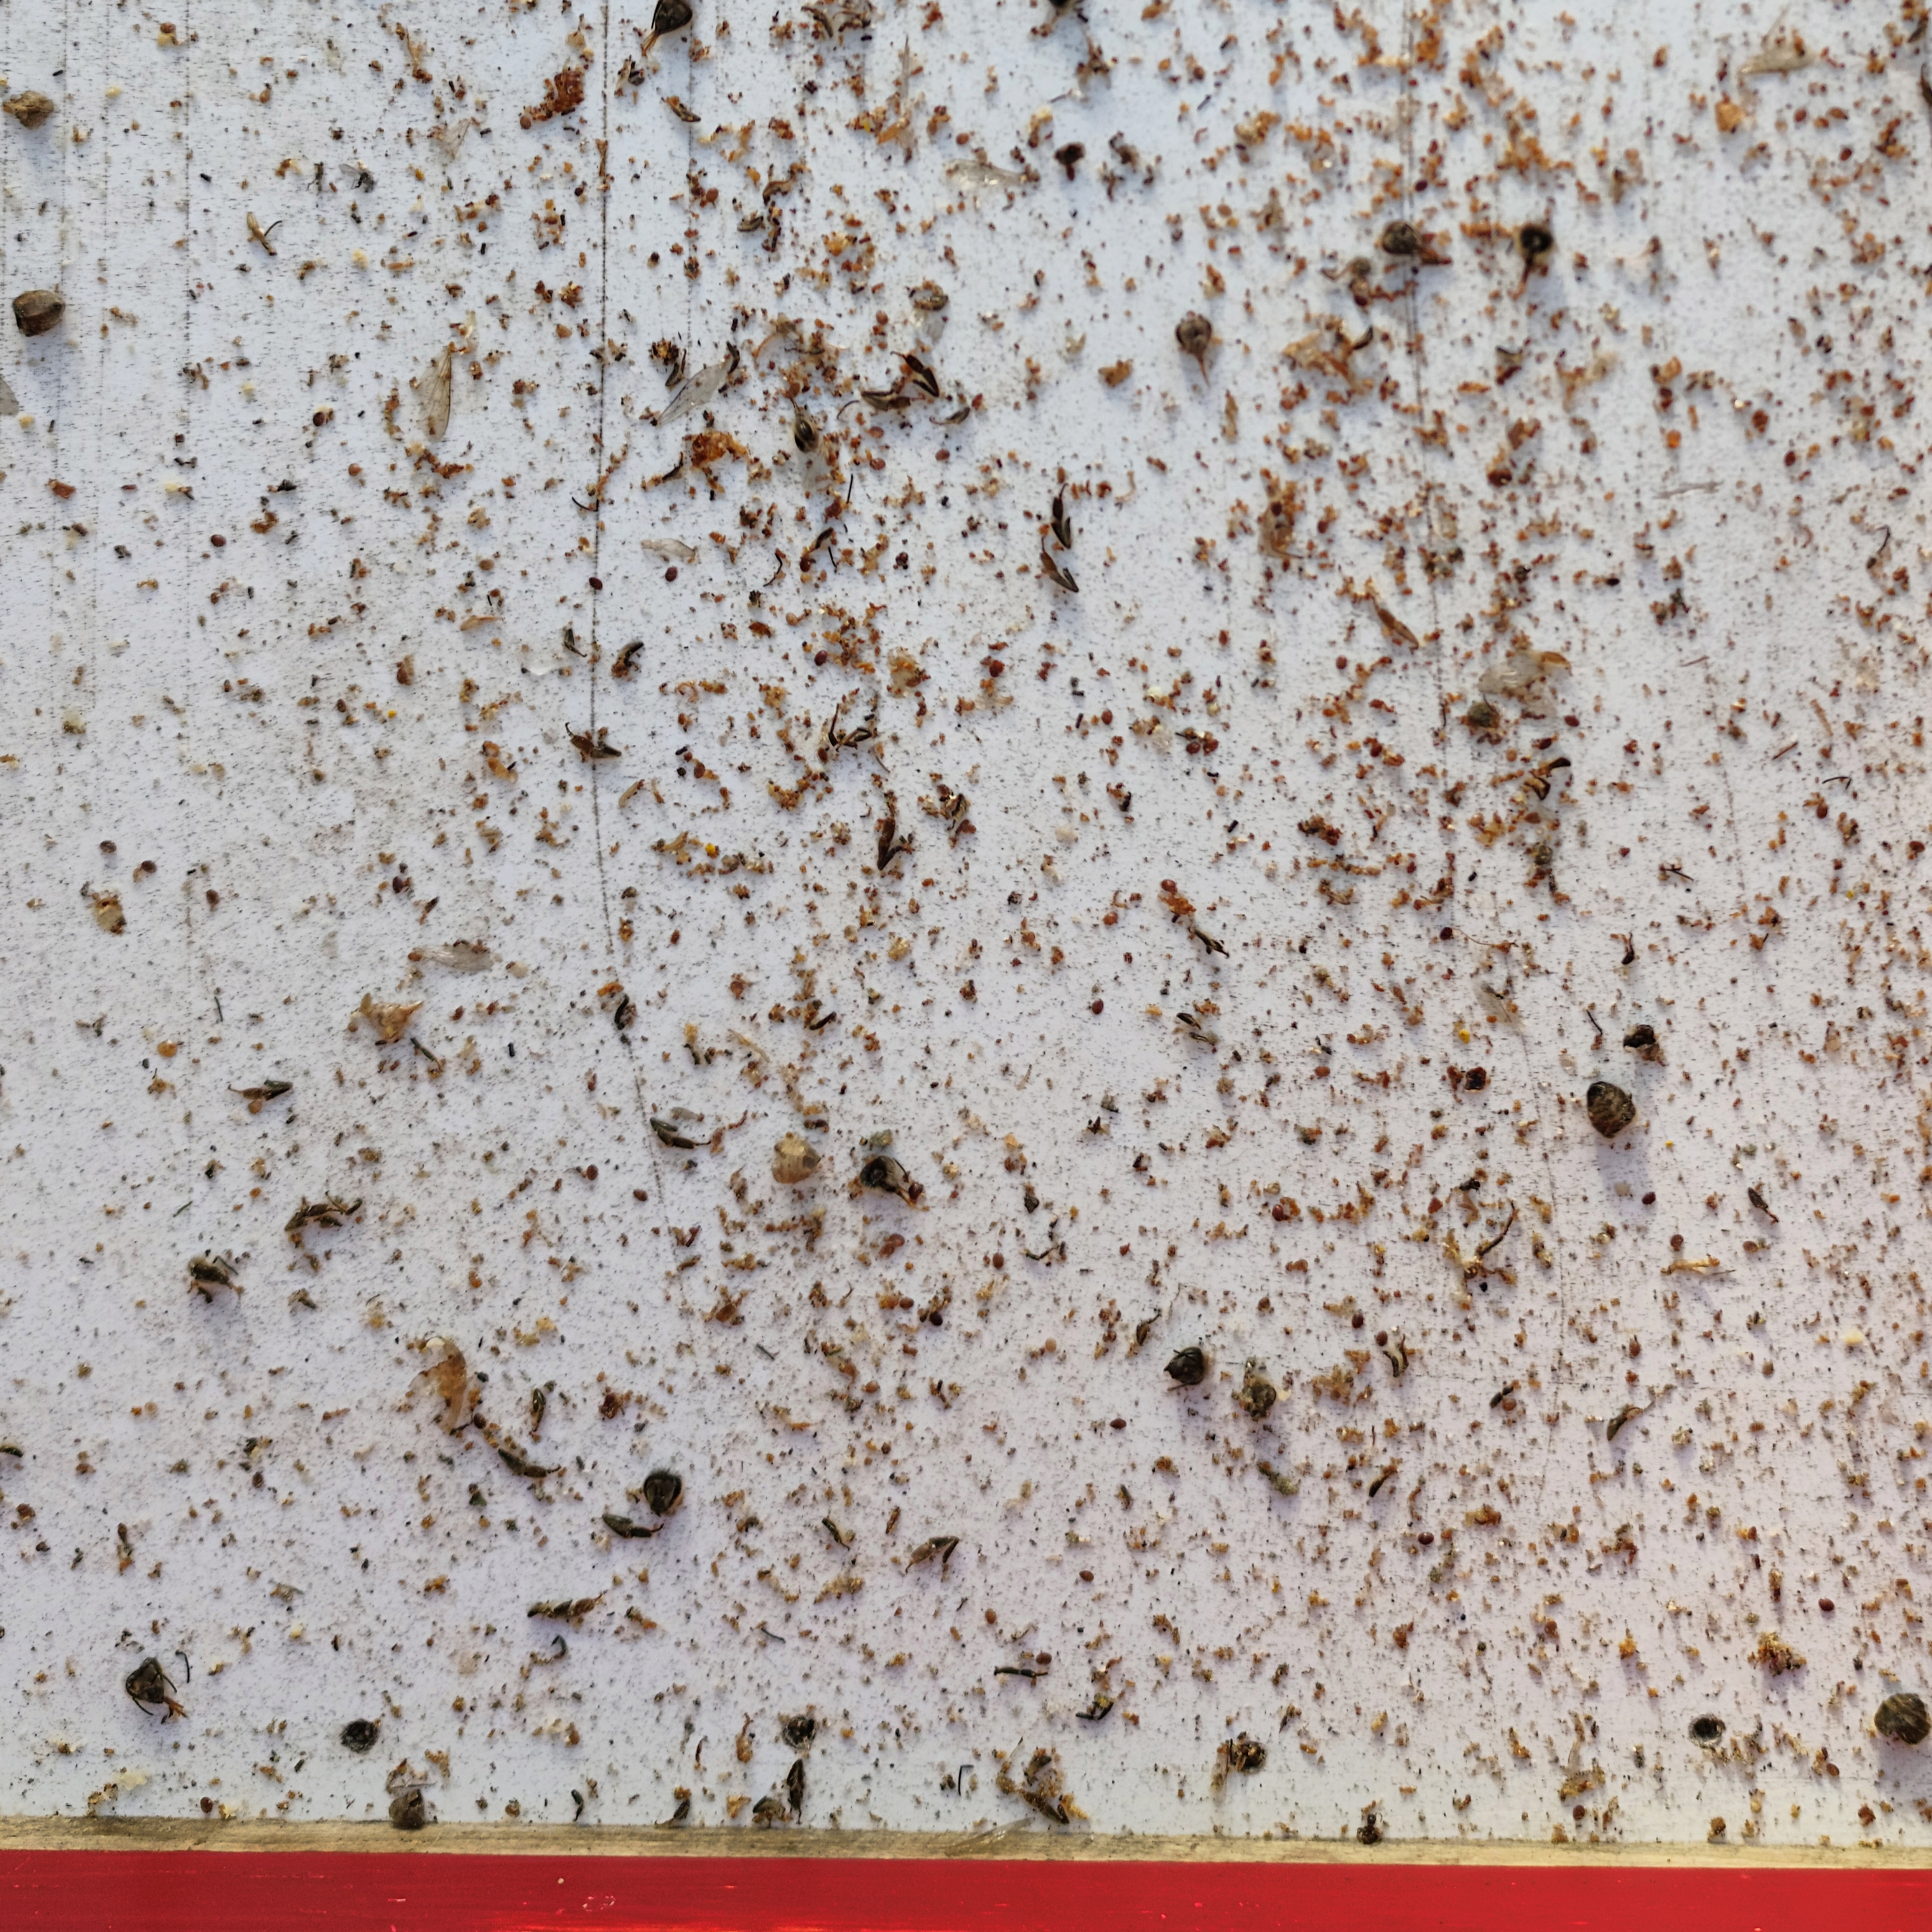
\includegraphics[width=\textwidth]{obrazky-figures/podlozka_zdrava.jpg}
        \caption{Zdravé včelstvo}
        \label{fig:podlozka_zdrava}
    \end{subfigure}\hfill\begin{subfigure}[b]{0.5\textwidth}
        \centering
        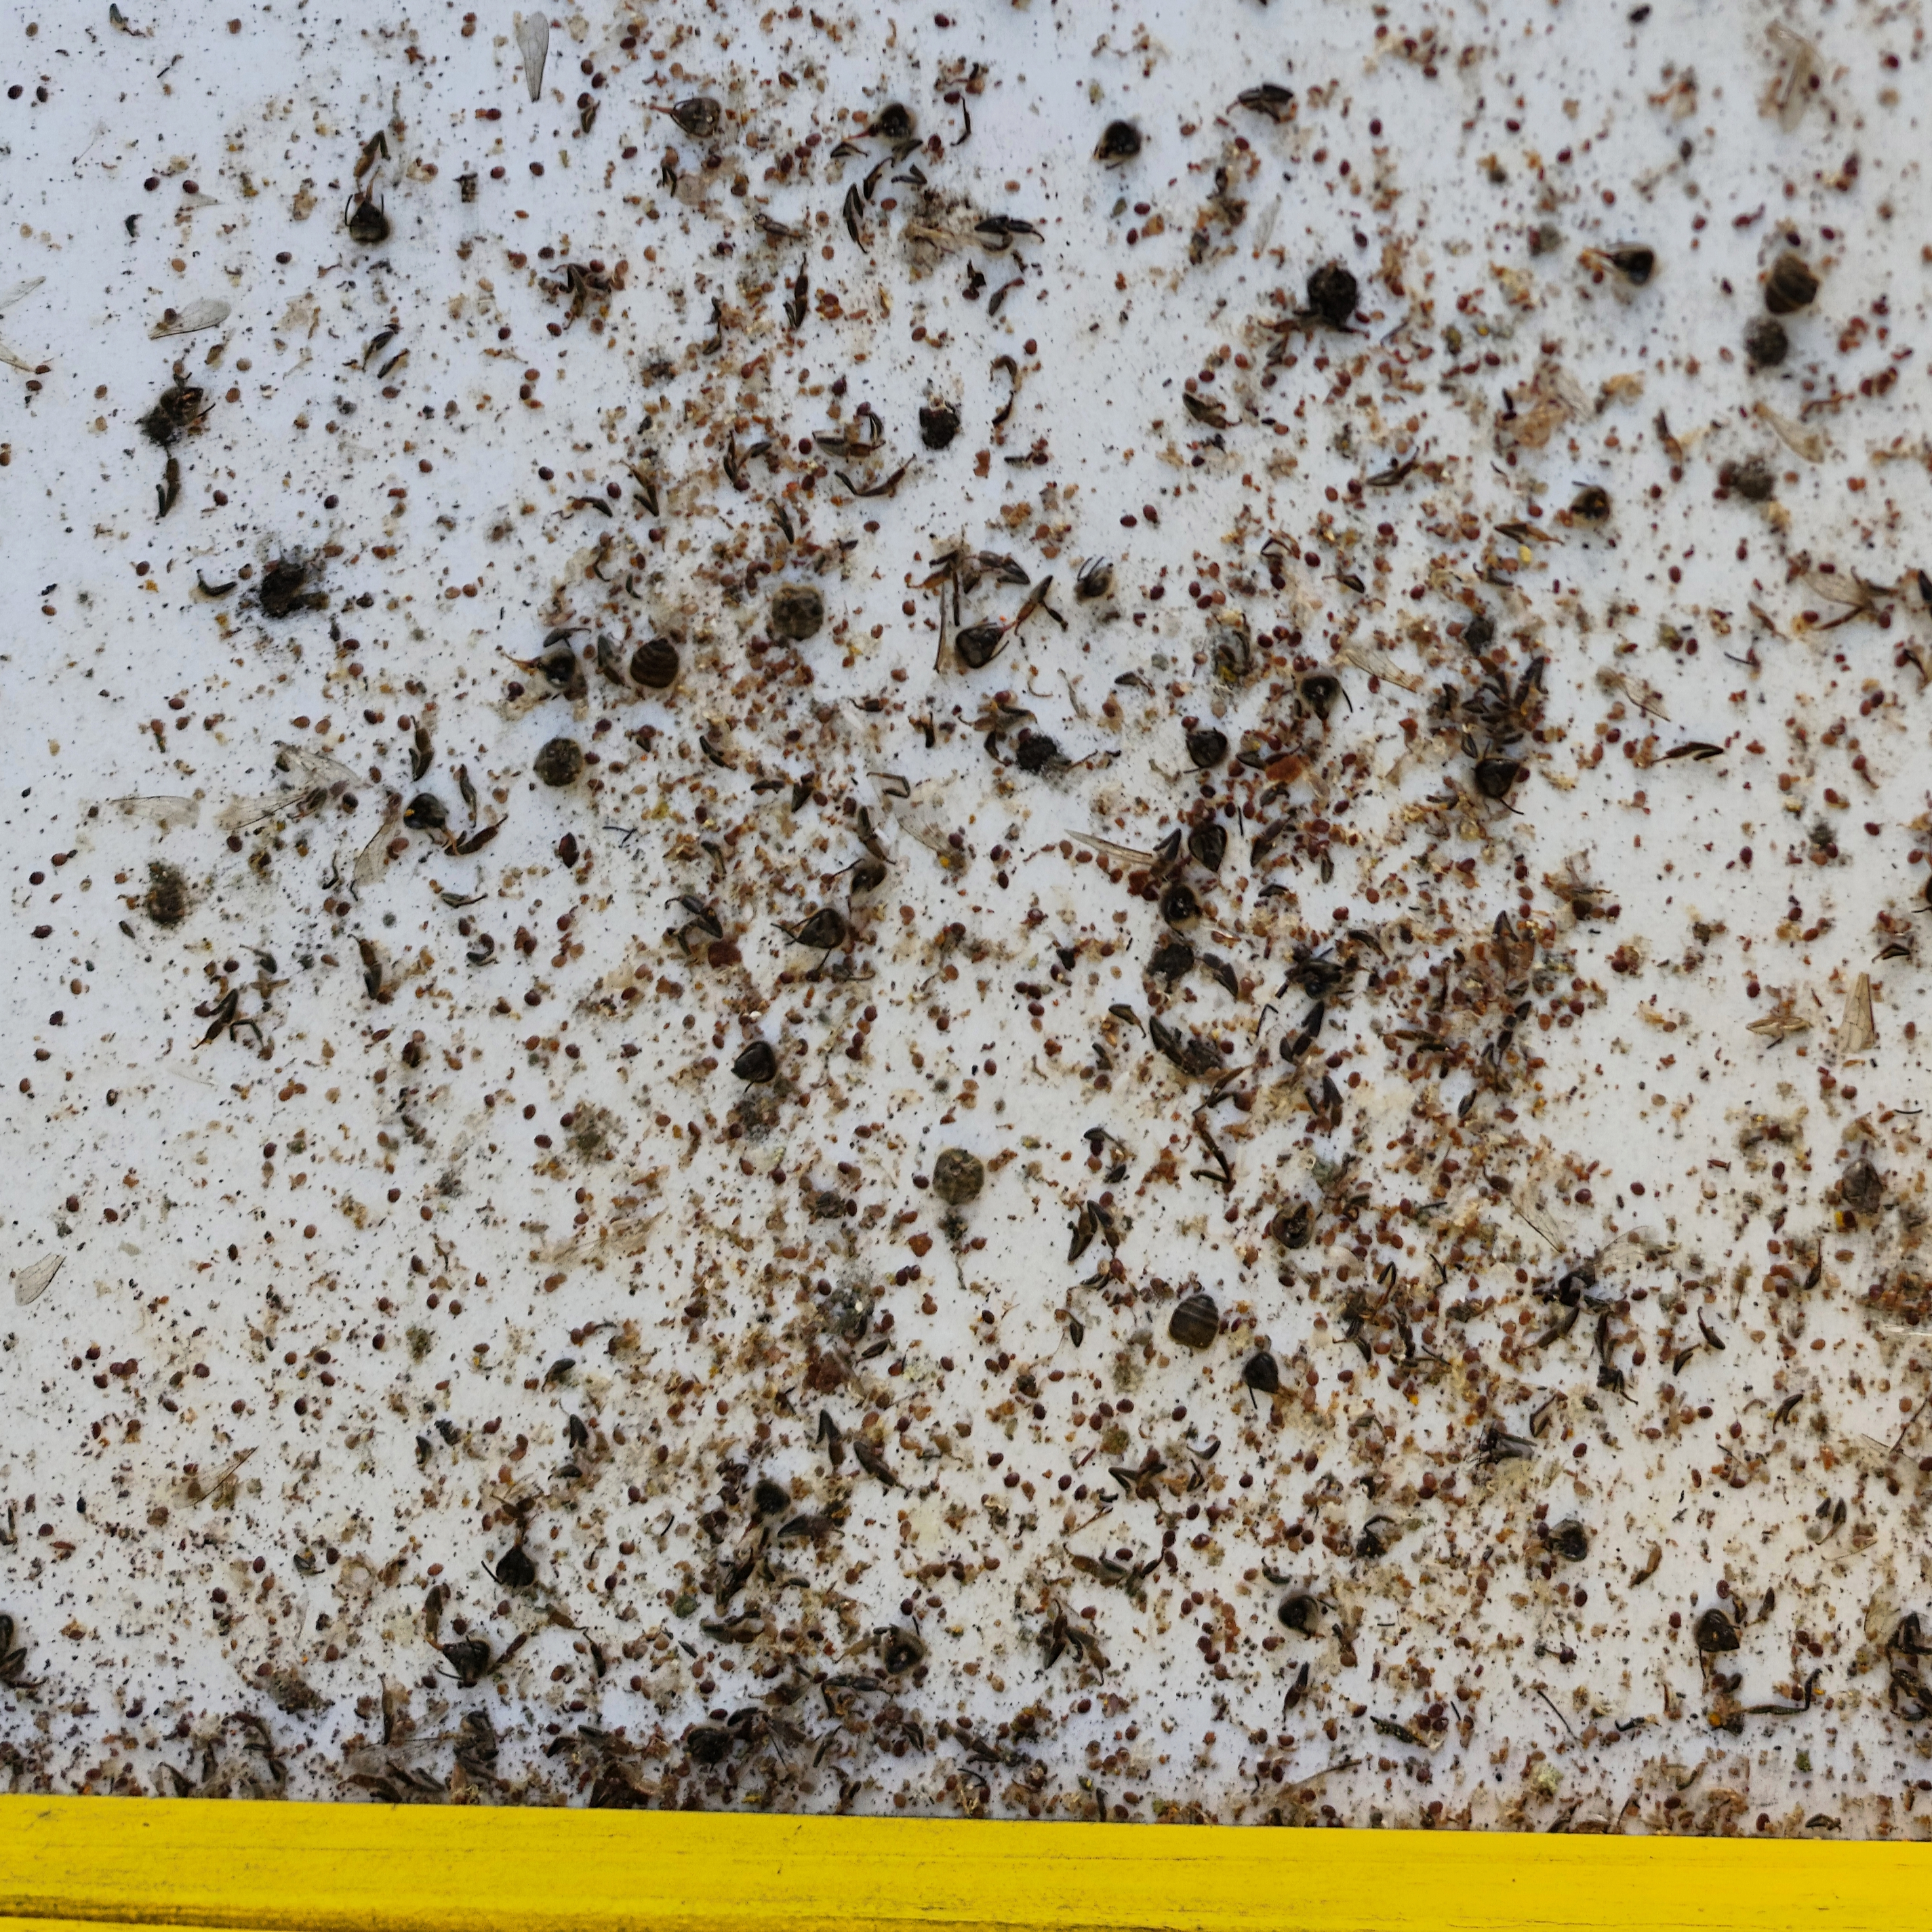
\includegraphics[width=\textwidth]{obrazky-figures/podlozka_napadena.jpg}
        \caption{Napadené včelstvo}
        \label{fig:podlozka_napadena}
    \end{subfigure}
	
	\caption{Srovnání podložky zdravého a napadeného včelstva při podzimním léčení. Vlevo podložka s~minimálním spadem roztoče \textit{Varroa destructor}, vpravo s~výrazným výskytem.}
	\label{fig:srovnani_spadu}
\end{figure}

\subsubsection*{Další onemocnění}
Mezi další nemoci lze zařadit mor včelího plodu. Jedná se o~vysoce nakažlivé bakteriální onemocnění zavíčkovaného plodu, jehož původcem je bakterie \textit{Paenibacillus larvae}. Dospělé jedince nenapadá, ti však mohou nemoc přenášet, například při loupežích v~jiných úlech. Nemoc může mezi jednotlivými koloniemi přenést i včelař, a to křížovou kontaminací při kontrolách.

Spóry této bakterie dokážou přežít v~prostředí úlu (plásty, med, úlové vybavení) až desítky let. K~nákaze dochází po pozření těchto spor larvami, jež následně umírají. Nákazu lze poznat propadlými a děravými víčky, hnilobou, zbytky plodů a zejména pak zápachem. Při silném rozvoji onemocnění postihuje většinu plodu, v~důsledku čehož včelstvo slábne a může až uhynout \cite{Ritter}.

Mor včelího plodu je považován za neléčitelné onemocnění, proto má mnoho zemí velmi striktní hygienická a likvidační opatření. Při nálezu výskytu ho musí včelař dle zákona neprodleně oznámit, z~postižené kolonie je odebrán vzorek a zaslán do laboratoře. Napadenou kolonii pak musí majitel zlikvidovat, typicky utracením včelstva a spálením veškerého kontaminovaného materiálu či dekontaminací ozářením \cite{csvMor}.

Existuje také evropský mor včelího plodu, který naopak napadá otevřený, nezavíčkovaný plod, jenž hyne ještě před zavíčkováním. Toto onemocnění ale nebývá vždy fatální pro celé včelstvo \cite{Ritter}.

\subsubsection*{Škůdci}
Nemoci a parazité nejsou tím jediným, co včelstva zatěžuje. Významnou roli v~této oblasti hrají různí škůdci, kteří samotné včely loví, rabují zásoby a zabíjejí larvy. I samotné včely často rabují okolní kolonie.

Vosy a sršně patří mezi nejvýznamnější přirozené predátory včel, protože napadají jak včely, tak i oslabená či špatně chráněná včelstva. Na včely si počkají před česnem, kde je loví a odnášejí jako potravu pro své vlastní larvy. Případně pronikají až dovnitř úlu, kde rabují med, pyl i plod. V~evropských podmínkách mezi hlavní druhy těchto škůdců patří vosa obecná (\textit{Vespula vulgaris}) a sršeň obecná (\textit{Vespa crabro}). 

Zdravé včelstvo si s~několika jedinci dokáže poradit samo. Proti sršním se například využívá zúžení vstupu do úlu kvůli jejich velikosti. Problém však v~poslední době tvoří jiný druh sršně, proti kterému se stala tato metoda ochrany neúčinná. Tím je sršeň asijská (\textit{Vespa velutina}), jedná se o~invazivní druh, který se rozšiřuje po Evropě. V~České republice se výskyt potvrdil na podzim roku 2023 \cite{svscrSrsenAsijska}. Je o~něco menší než sršeň obecná a redukce česna ji proto nedokáže zastavit. Evropské včely se proti ní samy bránit příliš nedokážou, proto mohou být útoky těchto predátorů pro včelstvo i fatální \cite{monceau2014}. Článek navíc uvádí, že ve Francii, kam byla sršeň do Evropy v~roce 2004 zavlečena, bylo v~roce 2010 oslabeno či zničeno 30\,\% úlů.

Z~řad drobnějších škůdců lze uvést například zavíječe voskového. Larvy tohoto motýla se živí voskem, zejména plásty, ve kterých se nachází včelí plod. Dále pak i mravenci, kteří si vytvářejí hnízda v~polystyrenové vrstvě zateplených úlů \cite{Ritter}.

V~neposlední řadě se jedná o živočichy, jako jsou ptáci nebo drobní hlodavci, kteří úl poškozují spíše mechanicky. V~zimě jej mohou vyhledávat jako úkryt a zdroj potravy.

\subsubsection*{Rojení}
Rojení představuje přirozený způsob rozmnožování včelstev, kdy se jedno silné včelstvo rozdělí na dvě nebo více částí. Typicky stará matka vytváří roj a úl opouští, aby ustoupila matce nové. Pro včelaře je velmi obtížné se na tuto událost připravit. Většinou se jí snaží předcházet s~využitím různých opatření, například rozšířením úlu, tedy přidáním takzvaných \textit{rámků s~mezistěnkou}, aby měly včely další prostor pro ukládání zásob. K~dalším opatřením se řadí přistřižení matčiných křídel \cite{ivcelarstviRojeni}. Nejdůležitější jsou však pravidelné prohlídky rámků, při nichž včelař kontroluje, zda včely nezakládají \textit{matečníky}, tedy buňky, ze kterých vyrostou včelí matky.

Rojení probíhá od jara až do konce června a lze jej rozdělit na \textit{prvoroj}, kdy vylétá stará matka, \textit{druhoroj}, kdy vylétá nová neoplozená matka. Někdy může dojít ještě k~dalším rojením: \textit{třetiroj} atd. Takové chování včel se nazývá \textit{rojová nálada}. K~jejím znakům se řadí velké množství včel, plodu, zásob a snůšky, také zakládání matečníků. Tyto buňky lze nalézt na spodní straně plástu a jsou výrazně větší než ostatní. Čas rojení nastává v~devátý den od zavíčkování matečníku \cite{Gerstmeier}.

I~přesto, že se jedná o~naprosto přirozený proces v~životě včelstva, je pro včelaře negativní, jelikož tím přichází o~velkou část zásob i létavek. Včelstvo pak zůstává oslabené a nová matka neklade vajíčka, protože ještě není oplodněná. Včelař má proto za cíl vyletělý roj chytit a buď z~něj vytvořit novou kolonii, nebo včely vrátit zpět k~té původní.

\section{Měřitelné veličiny} \label{sec:veliciny}
Moderní přístupy k~monitorování včelstev se opírají o~kontinuální měření fyzikálních veličin přímo v~úlu či jeho bezprostřední blízkosti. Přitom žádná veličina není sama o~sobě dostačující pro poskytnutí uceleného obrazu o~stavu dané kolonie -- teprve jejich kombinace a sledování v~čase umožňuje rozpoznat jak normální průběh včelařského roku, tak odchylky značící problém \cite{Cecchi}.

V~rámci systémů využívajících senzory pro monitoring se nejčastěji měří hmotnost, teplota a relativní vlhkost. Některá zařízení přidávají ještě měření atmosférického tlaku, zvuku, oxidu uhličitého či aktivity na česně \cite{Sabic2025}. V~následující části textu jsou popsány základní veličiny -- jejich způsob měření, typické hodnoty v~průběhu roku a znaky rizikových stavů.

\subsubsection*{Hmotnost}
Hmotnost celého úlu je jednou z~veličin s~nejvyšší informační hodnotou, kterou lze při monitorování včelstev sledovat. Měří se pomocí takzvaných \textit{úlových vah}, tedy tenzometrickým snímačem umístěným pod úlem. Získaná data se pak často přenášejí do vzdáleného úložiště. Výhodou tohoto způsobu měření je, že nevyžaduje žádný zásah do úlu a může probíhat nepřetržitě po celý rok.

Hmotnost se v~průběhu roku mění v~závislosti na sezóně. Na jaře a v~létě, v~době snůšky, dochází k~pravidelnému přírůstku -- včely nosí pyl a nektar, matka klade vajíčka a zásoby přibývají. Zároveň dochází i k~denním změnám: v~ranních hodinách hmotnost poklesne, když včely opouštějí úl. Ve večerních hodinách naopak stoupá, jak se včely vracejí s~nektarem \cite{Cecchi}. V~zimním období naopak hmotnost pozvolna klesá, protože včelstvo spotřebovává zásoby. Průměrná zimní spotřeba se pohybuje okolo 6--15 kg, v~závislosti na velikosti kolonie a délce zimního období \cite{domaciVcelarstvi}. 

\begin{figure}[H]
	\centering
    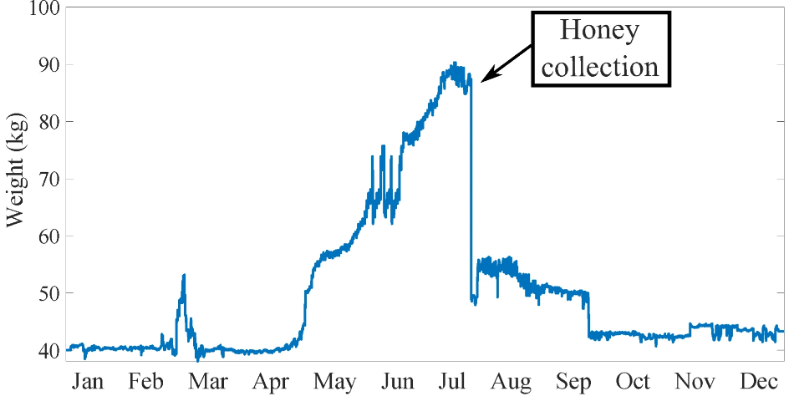
\includegraphics[width=0.5\textwidth]{obrazky-figures/hmotnost_rocni.png}
	\caption[Roční průběh hmotnosti úlu.]{Roční průběh hmotnosti úlu.\footnotemark}
	\label{fig:hmotnost_rocni}
\end{figure}
\footnotetext{Graf pochází z~\cite{Cecchi}, Obrázek 3d.}

Právě v~interpretaci odchylek od těchto očekávaných vzorců spočívá největší přínos průběžného vážení. Náhlý pokles hmotnosti v~řádu 3--4 kg, který lze vidět na obrázku \ref{fig:hmotnost_rojeni}, bývá charakteristickým příznakem rojení. Velká část \textit{létavek} i stará matka úl opouštějí, čímž se jeho hmotnost jednorázově výrazně sníží \cite{Cecchi}. Tento projev je na hmotnostní křivce dobře identifikovatelný a může sloužit jako základ pro včasné upozornění včelaře, který tak může roj odchytit nebo alespoň reagovat na pozměněný stav včelstva.

\begin{figure}[H]
	\centering
    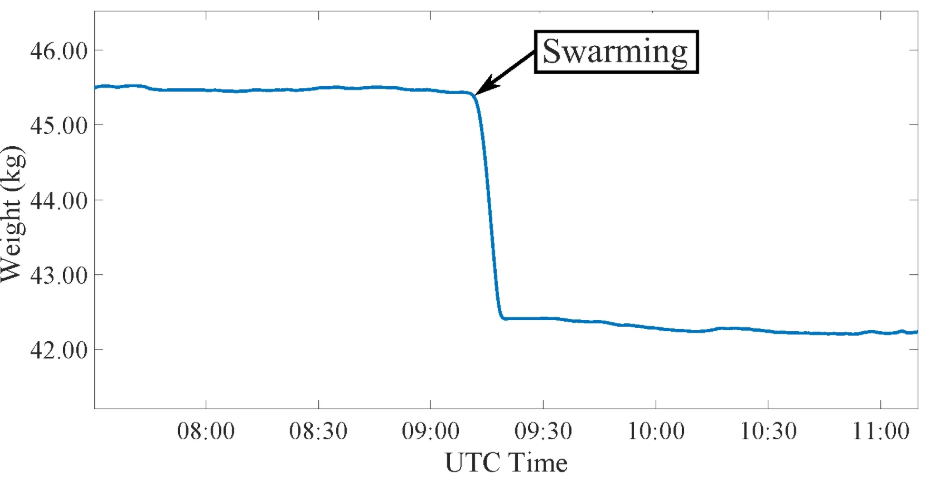
\includegraphics[width=0.5\textwidth]{obrazky-figures/hmotnost_rojeni.png}
	\caption[Změna hmotnosti při události rojení.]{Změna hmotnosti při události rojení.\footnotemark}
	\label{fig:hmotnost_rojeni}
\end{figure}
\footnotetext{Graf pochází z~\cite{Cecchi}, Obrázek 12a.}

Dále pak postupný úbytek hmotnosti mimo zimní období může znamenat hladovění kolonie, kdy včelám nestačí vlastní zásoby a je potřeba přikrmování. Naopak náhlý a extrémní pokles hmotnosti téměř na nulu může indikovat krádež nebo převrácení úlu \cite{dsouza2023hivelinkiotbasedsmart}.

Při sledování těchto změn hmotnosti v~čase je však vždy důležitý sezónní kontext, jelikož stejná změna může mít zcela jiný význam například v~lednu a v~červenci. Z~hlediska datové kvality se ukazuje jako vhodné pracovat s~průměry za delší časové intervaly nebo provádět měření ve stejnou denní dobu, protože surová data mohou obsahovat výrazný šum způsobený pohybem včel, větrem nebo vibracemi \cite{Cecchi}.

\subsubsection*{Teplota}
Teplota je veličinou, která odráží biologickou aktivitu včelstva nejpříměji, míněna je samozřejmě teplota uvnitř úlu. Okolní teplota slouží spíše jako kontext k~hodnotám hmotnosti či letové aktivity (nízká teplota znamená nízkou aktivitu včel). Včely disponují schopností aktivně regulovat teplotu uvnitř úlu v~závislosti na aktuálních potřebách včelstva \cite{Tautz2021}. Měření teploty proto poskytuje přímý vhled do fyziologického stavu kolonie.

Pro měření se nejčastěji využívá digitálních teplotních senzorů, případně kombinovaných, které kromě teploty měří i další veličiny, jako relativní vlhkost či atmosférický tlak. Zásadní roli hraje i umístění senzoru: nejpřesnější informace o~stavu plodového hnízda poskytuje senzor umístěný přímo uprostřed meziplástového prostoru v~centru úlu. Gradient teploty uvnitř úlu je přitom velmi výrazný -- od středu k~okrajům může dosahovat i 10--15\,°C \cite{Stabentheiner2021}, proto systémy s~více senzory poskytují lepší obraz o~stavu kolonie.

V~době, kdy matka klade vajíčka a v~úlu se nachází plod, udržují včely v~plodovém hnízdě teplotu v~úzkém rozmezí 34--36\,°C \cite{Stabentheiner2021} (kniha \textit{Fenomenální včely} \cite{Tautz2021} uvádí interval 33--36\,°C). Tato hodnota podmiňuje správný vývoj larev a kukel. Odchylky od zmíněné teploty mohou mít negativní dopad na kvalitu vylíhnutého plodu. Existence stabilní teploty v~tomto rozmezí je proto spolehlivým nepřímým ukazatelem přítomnosti matky a aktivity plodového hnízda. Naopak pokles teploty v~centru úlu pod 30\,°C v~průběhu hlavní sezóny by měl být signálem k~fyzické kontrole, jelikož může naznačovat ztrátu včelí matky nebo jiný závažný stav kolonie.

V~zimním období včely netvoří aktivní plodové hnízdo a shlukují se do tzv. \textit{zimního chomáče}. Ten funguje jako živý izolátor: teplota v~jeho středu se pohybuje okolo 15--25\,°C \cite{Gerstmeier}, zatímco na povrchu může klesnout k~10\,°C. To je totiž teplota, při níž včely ztrácejí schopnost pohybu \cite{Tautz2021}. Postupný nárůst teploty od přelomu ledna a února signalizuje, že matka opět začíná klást vajíčka a včelstvo se připravuje na jaro.

Teplotní data jsou také jedním z~nejspolehlivějších indikátorů blížícího se úhynu kolonie. Studie Minaud et al. \cite{Minaud} ukázala, že sledování teplotní variability uvnitř úlu v~průběhu zimování umožňuje s~přesností přes 96,8\,\% rozlišit přezimující kolonie od těch, které zimu nepřežijí. Umírající včelstvo postupně ztrácí schopnost udržovat potřebnou teplotu, včely ztrácejí schopnost pohybu a vnitřní teplota se přibližuje teplotě venkovní, viz obrázek \ref{fig:teplota_zima_uhyn}.

\begin{figure}[H]
	\centering
    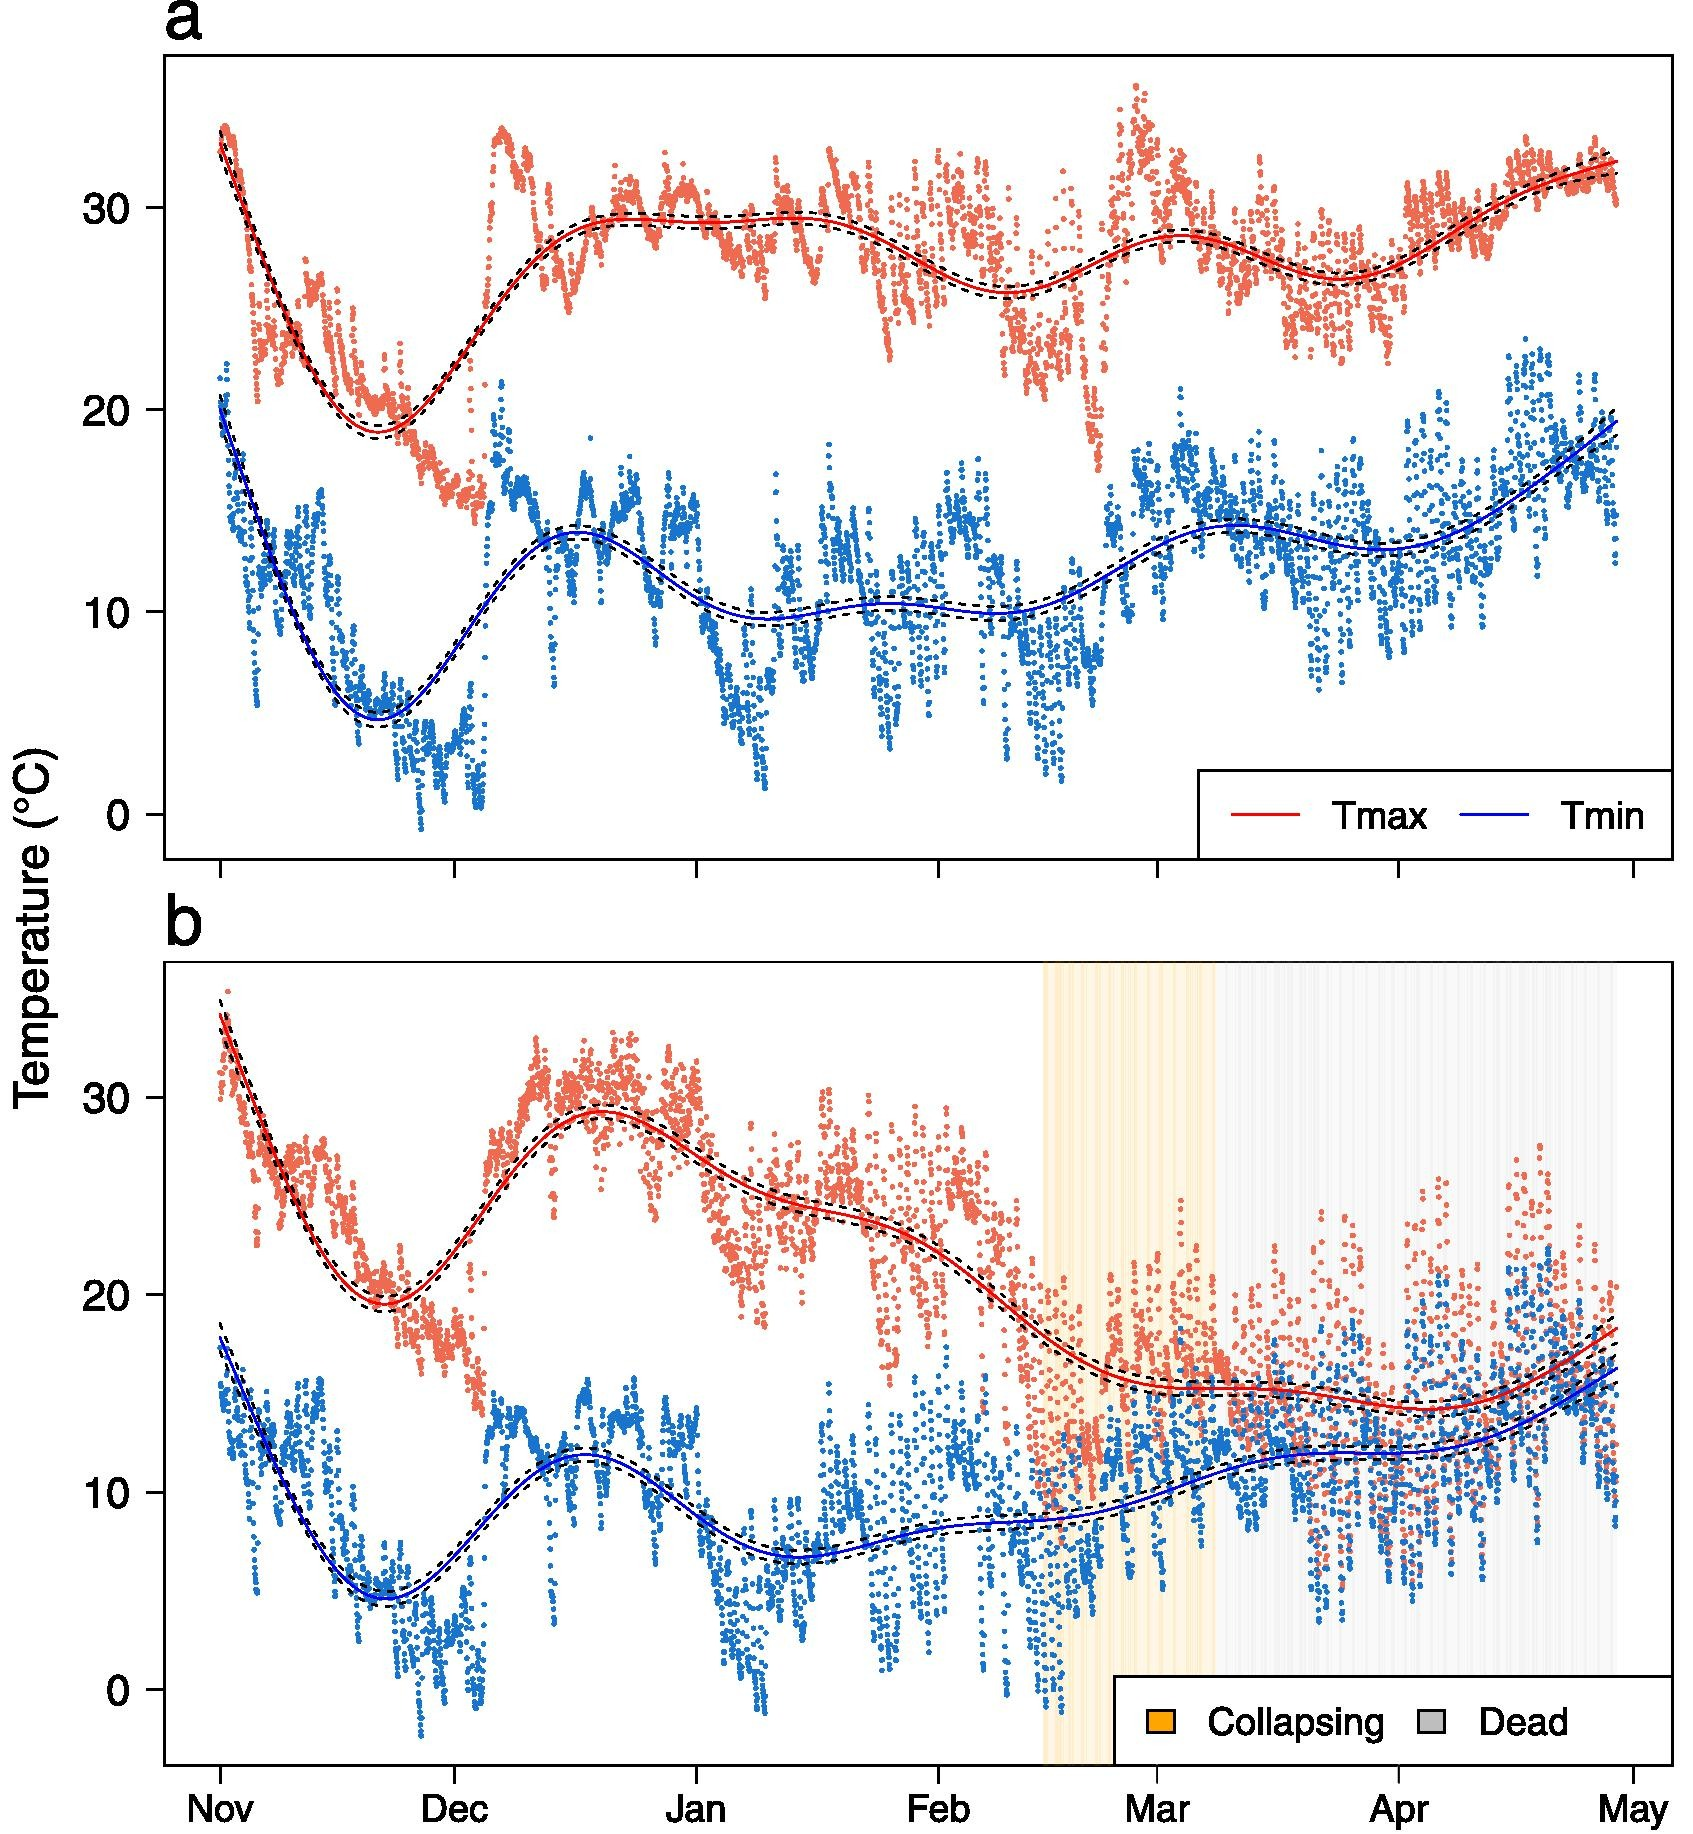
\includegraphics[width=0.6\textwidth]{obrazky-figures/teplota_zima_uhyn.jpg}
	\caption[Porovnání zdravého (a) a uhynulého (b) včelstva v~zimním období.]{Porovnání zdravého (a) a uhynulého (b) včelstva v~zimním období.\footnotemark}
	\label{fig:teplota_zima_uhyn}
\end{figure}
\footnotetext{Grafy pochází z~\cite{Minaud}, Obrázek 2.}

Naopak krátkodobý nárůst teploty v~kombinaci s~nárůstem vlhkosti může předcházet samotnému odletu roje. Roj se zahřívá, a až jeho teplota stoupne na 35\,°C, vyletí ven \cite{Tautz2024}. Včely před rojením větrají úl (víření křídel na česně) a zvyšují svou pohybovou aktivitu, což se projeví i na senzorech \cite{Cecchi}.

V~letních měsících může naopak přílišné horko způsobit, že včely začnou intenzivně větrat česno. Pokud tyto snahy nestačí, včely se na česně začnou ve větším množství shromažďovat. V~extrémních případech je nutný zásah včelaře \cite{Stabentheiner2021}.

\subsubsection*{Relativní vlhkost} \label{veliciny-vlhkost}
Ačkoliv se může na první pohled zdát, že se jedná o~veličinu, která není tolik důležitá, relativní vlhkost úzce souvisí s~několika klíčovými procesy v~životě kolonie. Měří se pomocí kapacitních senzorů. Praktickým problémem při dlouhodobém nasazení jsou samotné včely, které mohou vnitřní senzory obalovat propolisem či voskem. To může způsobovat odchylky měření až úplný výpadek senzoru, což lze následně pozorovat například na grafu naměřených hodnot. Tento jev byl zdokumentován při měření plynů v~úlu \cite{Rigakis2023} a autoři problém vyřešili uložením senzoru do ochranné krabičky.

Nejzásadnější funkcí regulace vlhkosti v~úlu je zpracování nektaru na med. Čerstvě přinesený nektar obsahuje 60--80\,\% vody. Aby byl med kvalitní a nezačal kvasit, musí včely jeho vlhkost snížit pod 20\,\% \cite{nettie}. Tohoto dosahují aktivním větráním. Díky tomuto procesu vlhkost v~úlu výrazně stoupá, zejména v~nočních hodinách, kdy odpařená voda zůstává uvnitř. Sledování nočního nárůstu vlhkosti může sloužit jako nepřímý indikátor intenzity snůšky.

Pro správný vývoj a přežití vajíček je nezbytná relativní vlhkost alespoň 55\,\% v~oblasti plodového hnízda, ideální je však až 90--95\,\% \cite{Linton2019}. Samotné plodové hnízdo udržují včely v~rozmezí přibližně 40--70\,\% RH prostřednictvím aktivního větrání \cite{Linton2019}. Dlouhodobá vlhkost výrazně přesahující tuto hranici, nebo naopak klesající pod 40\,\% může signalizovat poruchu regulačního mechanismu, tedy oslabení nebo zmenšení kolonie.

V~zimním období představuje nadměrná vlhkost jedno z~rizik, která mohou přezimující včelstvo oslabit nebo poškodit. Kondenzace vlhkosti na stěnách úlu a plástech může vést ke tvorbě plísní, poškození zimních zásob nebo přímo k~navlhnutí chomáče, což výrazně zvyšuje energetické nároky na jeho vytápění \cite{Linton2019}. Správné větrání úlu v~zimě proto není jen otázkou eliminace vlhkosti z~dechu včel, ale přímo podmínkou úspěšného přezimování.

Relativní vlhkost může být také jedním z~indikátorů předcházejícího rojení. Bezprostředně před odletem roje bylo v~některých měřeních zaznamenáno krátkodobé zvýšení jak teploty, tak vlhkosti uvnitř úlu \cite{Cecchi} -- pravděpodobně v~důsledku zvýšené aktivity a tělesného tepla shlukujících se rojových včel. Samotná vlhkost však nestačí jako jediný prediktor, proto je vhodné ji kombinovat s~teplotou či dalšími veličinami.

\subsubsection*{Letová aktivita}
Letová aktivita představuje počet včel procházejících česnem za jednotku času a jejich směr pohybu. Jedná se o~veličinu odrážející vnější sběrací část včelstva. Zatímco teplota a hmotnost informují převážně o~dění uvnitř úlu, letová aktivita zachycuje, jak intenzivně kolonie komunikuje s~okolním prostředím \cite{Meikle2015}. Z~biologického pohledu zodpovídají za letovou aktivitu včely \textit{létavky}. Právě letová aktivita proto úzce souvisí s~dostupností snůšky v~okolí a s~celkovou silou a zdravotním stavem kolonie.

Principů pro automatizované měření této veličiny existuje celá řada. Mezi historicky nejpoužívanější patří infračervené senzory nebo fotoelektrické závory. Modernější přístupy zahrnují kapacitní senzory, RFID čipy přilepené na hrudní část jedinců, které umožňují sledování konkrétních včel, kamerové systémy zpracovávající video pomocí algoritmů pro sledování objektů nebo Dopplerův radar. Podrobnější informace uvádí sekce \ref{senzor-let}. Každá z~metod má své výhody i nevýhody týkající se přesnosti, invazivnosti, náročnosti zpracování či citlivosti na změny osvětlení nebo počasí \cite{Williams2023}.

Letová aktivita silně závisí na vnějších podmínkách, zejména na teplotě a intenzitě slunečního záření. Včely typicky nelétají při teplotách pod 10\,°C, při dešti nebo silném větru. Studie Clarke et al. \cite{Clarke2018} ukázala, že teplotou a slunečním zářením lze vysvětlit až 78\,\% variability v~letové aktivitě měřené na česnu. Tato silná závislost na počasí je na jedné straně praktickým omezením, protože naměřené hodnoty musíme interpretovat v~kontextu aktuálních meteorologických podmínek, na druhé straně právě odchylky od předpovídané aktivity mohou být chápány jako rizikový stav \cite{Meikle2015}.

Takové stavy jsou například snížená aktivita při jinak příznivém počasí, což může naznačovat oslabení kolonie, ztrátu létavek v~důsledku otravy pesticidy nebo přítomnosti predátora.

Jarní nárůst letové aktivity bývá také jedním z~nejdříve pozorovatelných signálů jarního rozvoje včelstva, a to ještě předtím, než jsou patrné změny na vahách. První orientační prolety, v~závislosti na geografické poloze, u~nás začínají přibližně od konce února, jakmile teplota překročí 10\,°C \cite{beeinfo}. V~rámci proletů se včely orientují a nosí první potravu. U~kamerových systémů lze dokonce určit dostupnost specifických druhů rostlin v~okolí úlů dle pylových roušek na zadních nožkách včel \cite{Cecchi}.

Největším praktickým omezením automatického sledování letové aktivity zůstává technická náročnost instalace a údržby senzorů. Zařízení mohou včely stresovat a ty je následně znečišťují, jak bylo zmíněno výše. Kamerové systémy jsou citlivé na venkovní světelné podmínky a vyžadují výpočetní kapacitu pro zpracování videa v~reálném čase nebo jeho archivaci. Proto se v~praxi letová aktivita měří spíše pro výzkumné účely, nikoli jako součást komerčních monitorovacích systémů pro běžné včelaře.

\section{Některá existující komerční řešení a jejich srovnání} \label{sec:komercni_reseni}
Současný trh s~technologiemi pro monitorování včelstev lze rozdělit do dvou základních kategorií. První tvoří modulární senzorová řešení, která se přidávají k~existujícímu úlovému vybavení -- typicky se jedná o~úlové váhy doplněné teplotními a vlhkostními senzory s~bezdrátovým přenosem dat. Druhou kategorii představují integrované inteligentní systémy, kde je monitorovací technologie nedílnou součástí samotného úlu, v~některých případech se jedná i o~prvky robotické automatizace. Zatímco první kategorie je zaměřena na standardního včelaře hledajícího dostupné rozšíření stávající praxe, druhá cílí na profesionální a komerční provozovatele. V~následující části textu je představeno několik komerčních řešení dostupných na trhu.

\subsubsection*{BeeSage}
Lotyšský produkt BeeSage HiveScale v2 je primárně hmotnostní systém s~důrazem na jednoduchost nasazení a mezinárodní dostupnost. Váha měří hmotnost úlu a okolní teplotu s~hodinovým intervalem, součástí zařízení je i GPS modul pro sledování polohy úlu, který slouží jako ochrana před krádeží. Zařízení komunikuje prostřednictvím SIM karty zahrnuté v~ceně (399 EUR) a data jsou dostupná přes webovou aplikaci s~možností exportu. Výrobce také pracuje na integraci akustického monitorování v~budoucích verzích produktu \cite{beesage}. 

\subsubsection*{VeluBee}
VeluBee je český produkt s~více než desetiletou historií vývoje. Aktuálně je ve~třetí generaci hardwaru a nabízí tři produktové varianty. VeluBee Hive je kompletní sada obsahující řídicí jednotku, jednu váhu a solární panel, cena začíná na 9900 Kč a zahrnuje roční licenci. VeluBee One je přídavná váha pro rozšíření stávající sestavy (od~7300 Kč). VeluBee LUNIT je specifická offline varianta s~displejem pro lokality bez internetového připojení (od~8200 Kč). Oproti jiným řešením nabízí výrazně širší softwarové funkce: webová a mobilní aplikace zahrnuje interaktivní grafy s~možností porovnání více úlů, automatickou detekci snůšky, detekci krádeže a vyrojení, včelařský deník s~fotogalerií, správu kolonií a exporty dat ve~formátu CSV. Systém podporuje připojení přes Wi-Fi i IoT sítě a nabízí možnost vzdáleného tárování (vynulování) váhy přes internet \cite{velubee}.

\subsubsection*{BeeHive Monitoring}
Slovenský e-shop BeeHiveMonitoring.com nabízí rozsáhlé produktové portfolio zahrnující jak standardní úlové váhy s~řídicí jednotkou pro jejich správu, tak specializované senzorové moduly. Takovým modulem je například produkt Hive Heart, který se vkládá přímo na~rámky v~úlu a zaznamenává teplotu, vlhkost a zvuky včelstva -- právě analýza akustického signálu umožňuje systému předpovídat blížící se rojení. Dalším zajímavým produktem je počítadlo včel u~česna s~mechanicky upraveným vstupem, který zajišťuje průchod pouze jediné včely v~daný okamžik, což umožňuje přesnější počítání, výrobce ale neuvádí, na~jakém principu počítání funguje \cite{beehivemonitoring}.

\subsubsection*{Beewise}
Izraelská společnost Beewise představuje systém zásadně odlišný od všech předchozích -- BeeHome™ není doplňkem k~existujícímu úlu, ale zcela autonomním inteligentním zařízením pro současný chov dvou až deseti včelstev. Systém je vymyšlen tak, aby dokázal pracovat zcela samostatně bez jakéhokoliv lidského zásahu. Je vybaven robotickou paží umožňující vzdálenou manipulaci s~rámky, systémem pro automatické doplňování krmiva, léčení varroázy prostřednictvím termické komory (bez použití chemikálií) a ochranou před pesticidy prostřednictvím dálkově ovladatelného uzávěru česna. Počítačové vidění poháněné umělou inteligencí nepřetržitě analyzuje snímky rámků až na~úroveň jednotlivých buněk a monitoruje počty včel. Výrobce uvádí, že systém dosahuje o~70\,\% nižší míry úhynu kolonií oproti konvenčnímu chovu \cite{beewise}.

\subsubsection*{Apisense}
Polský systém Apisense představuje unikátní přístup orientovaný primárně na~chemické složení vzduchu uvnitř úlu. Zařízení je umístěno přímo na~rámek a kontinuálně analyzuje koncentrace organických sloučenin, oxidu uhličitého a oxidů dusíku, které fungují jako indikátory zdravotního stavu kolonie -- výrobce deklaruje 95\,\% úspěšnost ve~včasné detekci onemocnění. Senzor je doplněn o~měření teploty, vlhkosti a zvuku. Ve spolupráci s~Evropskou kosmickou agenturou (ESA) je plánována i satelitní analýza okolí stanoviště pro identifikaci zdrojů nektaru a potenciálních rizik (například zemědělské plochy ošetřované pesticidy). Data jsou přenášena prostřednictvím LTE brány. Výrobce nabízí výzkumný program, v~jehož rámci jsou zájemcům zasílána zařízení zdarma výměnou za závazek spolupráce a pravidelného odesílání dat \cite{apisense}.

\subsubsection*{ApiVčelař 4.0}
Česká firma ApiCo, s.r.o., která vznikla na~základě projektu Vysokého učení technického v~Brně, nabízí ekosystém dvou vzájemně propojených IoT zařízení v~rámci platformy ApiVčelař 4.0. Prvním produktem je úlová váha ApiVáha v~nerezovém provedení zajišťující celoroční bezúdržbový provoz a je kompatibilní se všemi typy úlů. Volitelným doplňkem je ApiSenzor umísťovaný přímo na~rámek uvnitř úlu, tento senzor monitoruje vnitřní teplotu, vlhkost i frekvenci. Druhým produktem je tracker ApiStopař, rovněž umísťovaný na~rámek, který kombinuje monitoring vnitřního mikroklimatu s~GPS sledováním polohy úlu -- při detekci otřesů nebo neoprávněné manipulace zasílá okamžité upozornění e-mailem i notifikací do mobilní aplikace. Obě zařízení komunikují prostřednictvím mobilní sítě (pro úlovou váhu existuje i offline varianta) a data jsou ukládána do cloudového úložiště. Přístup do úložiště a datový paušál jsou první rok součástí ceny zařízení, v~dalších letech jsou zpoplatněny částkou 528 Kč ročně \cite{apivcelar}.

\begin{table}[H]
    \centering
    \rotatebox{90}{
        \begin{tabular}{|m{2,8cm}|m{3,1cm}|m{2,2cm}|m{2,3cm}|m{2,4cm}|m{3,8cm}|}
        \hline
            \textbf{Název zařízení} & \textbf{Měření} & \textbf{Aktualizace dat} & \textbf{Komunikace} & \textbf{Napájení} & \textbf{Cena} \\
            \hline
            BeeSage HiveScale v2 & hmotnost, vnější teplota, poloha GPS & 1 hodina & GSM & dobíjecí baterie (USB) & od 399 € (9703,48 Kč)\,\footnotemark[4] \\
            \hline
            VeluBee Hive & hmotnost, vnější a vnitřní teplota & nastavitelné & Wi-Fi, IoT síť LTE & baterie + solární panel, napájení ze sítě & od 9900 Kč  \\
            \hline
            VeluBee LUNIT & hmotnost & okamžitě (diplej) & offline & dobíjecí baterie (USB) & od 8200 Kč \\
            \hline
            Kovová úlová váha & hmotnost, venkovní teplota a vlhkost & 10 minut & Bluetooth, GSM & dobíjecí baterie & 166,25 € (4043,12 Kč)\,\footnotemark[4] \\
            \hline
            Hive Heart & vnitřní teplota a vlhkost, zvuk & 10 minut & Bluetooth, GSM & baterie & 54,04 € (1311,50 Kč)\,\footnotemark[4] \\
            \hline 
            Počítadlo včel & počet včel & 10 minut & Bluetooth, GSM & baterie & 146,58 € (3564,75 Kč)\,\footnotemark[4] \\
            \hline
            BeeHome™ & hmotnost, teplota, vlhkost, kamerový záznam rámků, pesticidy & nepřetržitě & neuvedeno & integrovaný systém se solárními panely & na vyžádání \\
            \hline
            Apisense & VOC\,\footnotemark[5], oxid uhličitý, oxidy dusíku, teplota, vlhkost, zvuk & neuvedeno & LTE & baterie & neuvedeno\\
            \hline
            ApiVáha & hmotnost, venkovní teplota & 30 minut & NB-IoT & baterie & 11690 Kč\\
            \hline
        \end{tabular}}
        \caption{Srovnání vybraných komerčních produktů pro monitorování včelstev.}
    \label{tab:porovnani_komercnich_produktu}
\end{table}

\footnotetext[4]{Měnový kurz platný ke dni 17. dubna 2026}
\footnotetext[5]{Zkratka VOC představuje označení pro těkavé organické sloučeniny}

\chapter{Hardwarové komponenty} \label{sec:hardware}
Kapitola se zaměřuje na výběr a popis hardwarových komponent, které jsou často využívány pro realizaci monitorovacího systému včelstev. Jsou zde představeny jednotlivé typy mikrokontrolérů a jednodeskových počítačů, které mohou sloužit jako řídicí jednotky systému, včetně jejich výhod a omezení z~hlediska výkonu, spotřeby a dostupnosti. Dále jsou diskutovány senzory určené pro měření fyzikálních veličin relevantních pro sledování stavu úlu, přičemž je kladen důraz na jejich přesnost, spolehlivost a vhodnost pro dlouhodobé nasazení v~terénu. V~neposlední řadě je řešena problematika napájení celého systému, zejména s~ohledem na autonomní provoz a možnost využití obnovitelných zdrojů energie, jako je solární napájení.

\section{Mikrokontroléry a jednodeskové počítače}
Výběr řídicí jednotky monitorovacího systému je jedním ze základních rozhodnutí celého návrhu. Na trhu existuje celá řada platforem lišících se výpočetním výkonem, spotřebou energie, konektivitou, cenou a ekosystémem softwarové podpory. Obecně lze tyto platformy rozdělit do dvou kategorií: \textit{mikrokontroléry} (MCU -- Microcontroller Units), tedy jednočipové systémy určené primárně pro přímé řízení hardwaru a senzorů s~nízkou spotřebou, a \textit{jednodeskové počítače} (SBC -- Single-Board Computers), které disponují plnohodnotným operačním systémem a jsou schopny zpracovávat složitější výpočetní úlohy \cite{PCBSync}. V~oblasti monitorování včelích úlů se nejčastěji setkáváme se třemi platformami: ESP32, Arduino a Raspberry Pi, přičemž každá z~nich nachází využití v~odlišné části systému nebo při odlišných požadavcích projektů.

\subsubsection*{ESP32}
ESP32 je rodina systémů na čipu (SoC) vyvinutá společností Espressif Systems, která se od~svého uvedení na trh v~roce 2016 stala jednou z~nejrozšířenějších platforem pro aplikace ~\textit{Internetu věcí} (IoT -- Internet of Things). Základ čipu tvoří dvoujádrový procesor Xtensa LX6 taktovaný na 240 MHz, integrovaná paměť SRAM o~velikosti 520 KB a paměť flash do 16 MB \cite{ESP32Datasheet}. Klíčovou vlastností, která ESP32 odlišuje od konkurenčních mikrokontrolérů, jako je Arduino, je integrovaná bezdrátová konektivita -- podpora Wi-Fi i Bluetooth bez~nutnosti externího komunikačního modulu \cite{ESP32Datasheet}.

V~kontextu monitorování úlů bývá ESP32 velmi oblíbenou volbou pro sběr dat ze senzorů a jejich odesílání do cloudu nebo na lokální server. Disponuje bohatou sadou periferií včetně rozhraní SPI, I2C, UART a PWM, které umožňují přímé připojení senzorů teploty, vlhkosti, váhových snímačů nebo kamer. Studie Hercog et al. \cite{Hercog2023} využívá právě modul na~bázi ESP32 (LilyGO TTGO T8) pro kompletní monitorovací systém úlu. Tento systém zahrnuje měření hmotnosti, teploty i vlhkosti a přenáší data přes mobilní GPRS síť na cloudovou platformu ThingSpeak. Schopnost ESP32 přecházet do režimů \textit{hlubokého spánku} (deep sleep) a probouzet se pouze v~okamžiku měření výrazně snižuje průměrnou spotřebu energie, což je klíčové pro nasazení se solárním napájením nebo baterií \cite{PCBSync}.

\subsubsection*{Arduino}
Arduino je otevřená hardwarová a softwarová platforma původně navržená pro výuku elektroniky a rychlé prototypování. Základní desky Arduino (například Uno nebo Nano) stojí na~8bitových mikrokontrolérech AVR od společnosti Microchip s~taktovací frekvencí 16 MHz a velmi omezenou pamětí -- Uno disponuje pouze 2 KB SRAM a 32 KB flash \cite{ArduinoUno}. Tato omezení sice výrazně zužují možnosti komplexního zpracování dat, na druhou stranu je Arduino díky obrovské komunitě, rozsáhlé knihovně hotových ovladačů a intuitivnímu vývojovému prostředí (Arduino IDE) ideální pro začátečníky a jednoduché senzorové aplikace.

V~oblasti monitorování úlů se Arduino uplatňuje zejména jako základní datový logger -- sbírá hodnoty ze senzorů a buď je ukládá lokálně na SD kartu, nebo předává nadřazené jednotce (například Raspberry Pi nebo ESP32). Standardní desky Arduino bez rozšiřujícího modulu bezdrátovou konektivitu nenabízejí. Je nutné přidat externí shield, což zvyšuje cenu i komplexitu zapojení \cite{ArduinoUno}. Novější modely řady Arduino MKR nebo Portenta tuto mezeru částečně vyplňují, ale za výrazně vyšší pořizovací cenu. Pro projekty vyžadující nízkou spotřebu, integrovanou konektivitu a vyšší výpočetní výkon tak ESP32 v~současné době ve~většině nových IoT nasazení nahrazuje právě Arduino \cite{PCBSync}.

\subsubsection*{Raspberry Pi}
Raspberry Pi je jednodeskový počítač (SBC) britské nadace Raspberry Pi Foundation, který na rozdíl od mikrokontrolérů jako ESP32 či Arduino spouští plnohodnotný operační systém -- standardně distribuci Linux Raspberry Pi OS (dříve Raspbian). To mu dává výrazně větší softwarovou flexibilitu: lze na něm provozovat databáze, webové servery, nástroje pro~strojové učení nebo zpracování videa, a programovat jej prakticky v~libovolném jazyce~\cite{RPiDoc}. 

\textbf{Raspberry Pi 4 Model B}, vydaný v~roce 2019, staví na čtyřjádrovém procesoru ARM Cortex-A72 taktovaném na 1,8 GHz a je dostupný ve~variantách s~1--8 GB operační pamětí LPDDR4-3200 \cite{RPi4ProductPage}. Konektivita zahrnuje Gigabit Ethernet port, Bluetooth 5.0, dva porty USB 3.0, dva porty USB 2.0, dva micro-HDMI výstupy, port CSI pro kameru a DSI pro displej. Standardní 40pinová lišta přináší zpětnou kompatibilitu s~předchozími generacemi a umožňuje připojení senzorů a rozšiřujících modulů \cite{RPi4Datasheet}.

\textbf{Raspberry Pi 5}, uvedený v~roce 2023, přináší výrazné zlepšení výkonu. Nový čtyřjádrový procesor ARM Cortex-A76 taktovaný na 2,4 GHz nabízí oproti Pi 4 znatelně vyšší výpočetní výkon. Paměť LPDDR4X-4267 běží na vyšší frekvenci, přidán byl konektor PCIe 2.0 umožňující připojení NVMe SSD (přes adaptér), a o~vstupně-výstupní operace se nově stará dedikovaný čip RP1, který výrazně zvyšuje propustnost USB a dalších periferií. Pi 5 vyžaduje napájení 5 V/5 A~(oproti 5 V/3 A~u~Pi 4) a při vyšší zátěži se doporučuje využít aktivní chlazení. GPIO lišta zůstává 40pinová a je zpětně kompatibilní s~Pi 4 \cite{Kitronik}.

\subsubsection*{Porovnání}
Volba mezi jednodeskovým počítačem a mikrokontrolérem není pouze otázkou výpočetního výkonu, ale také několika dalších aspektů. ESP32 vyniká nízkou spotřebou energie, integrovanou bezdrátovou konektivitou a přímým řízením senzorů s~bateriovým či solárním napájením. Jeho spotřeba v~aktivním režimu se pohybuje pod 1 W, zatímco Raspberry Pi při~běžném provozu typicky odebírá 3--5 W \cite{Serepas2025}. Arduino zůstává relevantní zejména pro~jednoduché senzorové aplikace nebo jako výukový nástroj, jeho omezený výkon a absence konektivity ho staví do nevýhody oproti například ESP32. Raspberry Pi naopak vyniká všude, kde je třeba spouštět složitý software, provozovat databázi nebo zpracovávat video. To je však za cenu vyšší spotřeby a nutnosti operačního systému. V~praxi se proto oba přístupy vzájemně doplňují a moderní monitorovací systémy pro včelí úly je kombinují.

\section{Senzory pro měření fyzikálních veličin}
Senzory představují základní stavební kameny každého monitorovacího systému pro včelí úl. Jejich výběr zásadně ovlivňuje přesnost naměřených dat, provozní spolehlivost, energetickou náročnost i celkovou cenu zařízení. Pro každou měřenou veličinu potom existuje celá řada typů senzorů, která se liší principem činnosti, komunikačním rozhraním, přesností a vhodností pro konkrétní nasazení. Přehled typů senzorů používaných v~existujících řešeních shrnuje článek Šabić et al. \cite{Sabic2025}, který analyzuje 135 publikací týkajících se monitorování úlů z~let 1995--2025.

\subsubsection*{Hmotnost}
Pro měření hmotnosti se v~monitorovacích systémech prakticky výhradně používají tenzometrické snímače, tzv. \textit{load cells}. Ty pracují na principu odporové tenzometrie. Kovové tělo snímače se při zatížení nepatrně deformuje, což mění odpor nalepených tenzometrů (odporových drátků) uspořádaných do Wheatstoneova můstku. Výstupní signál je velmi slabý (v~řádu mV) a vyžaduje zesílení a digitalizaci specializovaným obvodem \cite{Trent2017}.

V~praxi se nejčastěji setkáváme se dvěma konfiguracemi. \textit{Jednobodový snímač} (single-point load cell) je kompaktní prvek vhodný pro střední nosnosti a platformové váhy, kde bývá zatížení přenášeno mimo osu snímače \cite{singlePoint}. \textit{Ohybový snímač} (bending beam) nebo \textit{smykový snímač} (shear beam) patří mezi robustnější varianty používané pro vyšší nosnosti od desítek do tisíců kilogramů \cite{LoadCells}. Pro monitorování včelího úlu, jehož hmotnost se typicky pohybuje v~rozmezí 20--80 kg, jsou vhodné ohybové či smykové snímače s~nosností 50--100 kg.

Analogový výstup snímače se zpracovává 24bitovým A/D převodníkem HX711, který tvoří de facto standard v~cenově nenáročných IoT váhových aplikacích. Disponuje integrovaným nízkošumovým zesilovačem a komunikuje s~mikrokontrolérem přes jednoduché dvoudrátové rozhraní (Clock + Data) \cite{hx711}. Rozlišení 24 bitů odpovídá teoreticky více než 16 milionům diskrétních hodnot, přičemž efektivní rozlišení je v~praxi výrazně nižší kvůli mechanickým vlastnostem snímače, teplotnímu driftu a elektromagnetickému rušení. Pro~spolehlivý provoz se proto doporučuje softwarové průměrování více vzorků a pravidelná rekalibrace pomocí referenční hmotnosti \cite{Cecchi}.

Hlavní nevýhodou tenzometrických snímačů v~reálném nasazení je citlivost na vlhkost a teplotní změny. To se týká zejména levnějších snímačů bez hermetického krytí, které mohou v~průběhu měření driftovat o~jednotky až desítky gramů. Pro přesné celosezónní sledování se doporučuje volit snímače s~certifikací alespoň IP65 nebo IP67.

\subsubsection*{Teplota}
Teplotní senzory lze v~kontextu IoT monitorování včelích úlů rozdělit do několika základních kategorií: termistory, integrované digitální senzory a kombinované senzory měřící více veličin současně.

\textbf{Termistory} (zejména typ NTC -- Negative Temperature Coefficient) jsou pasivní odporové prvky, jejichž odpor exponenciálně klesá s~rostoucí teplotou. Bývají cenově dostupné, malé a mají rychlou odezvu, ale vyžadují analogový vstup mikrokontroléru, kalibraci a kompenzaci nelinearity převodní charakteristiky \cite{bhageria2026}. V~mnoha IoT aplikacích bývají nahrazovány digitálními alternativami.

\textbf{DS18B20} je digitální integrovaný obvod od firmy Maxim Integrated komunikující protokolem 1-wire. Jako jeho klíčovou vlastnost lze uvést možnost zapojení až desítek čidel na~jediný datový pin mikrokontroléru -- každé čidlo má unikátní adresu \cite{randomNerdTutorials}. Přesnost je továrně kalibrována na $\pm0{,}5$\,°C v~rozsahu $-10$ až $+85$\,°C (jinak je ale celkový teplotní rozsah $-55$ až $+125$\,°C), rozlišení lze měnit programově od 9 do 12 bitů \cite{bhageria2026}. Senzor také existuje ve vodotěsném provedení (zalitý v~nerezové sondě), díky tomu bývá často využíván i pro~měření teploty uvnitř úlu, například v~meziplástovém prostoru, kde je vystaven jak vlhkosti, tak i propolisu. Zmíněné použití lze vidět i v~článku o projektu \textit{BeeObserver} od Senger et al. \cite{BeeObserver}. Nevýhodu tvoří konverzní latence až 750 ms při nejvyšším rozlišení \cite{DS18B20datasheet}. V~praxi se mohou vyskytnout chybné hodnoty (např. $-127$\,°C) v~případě poruchy komunikace, které se musí ošetřit softwarově.

\textbf{BME280} od Bosch Sensortec je kombinovaný senzor měřící teplotu, relativní vlhkost a atmosférický tlak přes rozhraní I2C nebo SPI. Má teplotní rozsah $-40$ až $+85$\,°C s~přesností $\pm1$\,°C \cite{BME280datasheet}. Mezi nevýhody patří mírné samozahřívání čipu v~aktivním režimu, které může způsobovat naměřené hodnoty o~1--3\,°C vyšší než skutečná okolní teplota. Tuto vlastnost lze potlačit přechodem do \textit{forced mode}, kdy čip provede měření a okamžitě přejde do spánkového režimu \cite{randomNerdTutorials}. Díky trojkombinaci veličin na jednom čipu bývá BME280 oblíbenou volbou pro~meteorologické stanice a komplexní monitorovací systémy.

\subsubsection*{Relativní vlhkost}
Senzory relativní vlhkosti pracují nejčastěji na kapacitním principu, digitální pak interně převádějí tuto změnu kapacitance na teplotně kompenzovanou hodnotu relativní vlhkosti \cite{zbotic}.

\textbf{DHT22} (nebo ekvivalentní AM2302) byl po mnoho let nejrozšířenějším cenově dostupným senzorem vlhkosti a teploty v~IoT komunitě. Komunikuje 1-wire protokolem, přesnost je specifikována na $\pm2$\,\% RH a $\pm0{,}5$\,°C \cite{DHT22datasheet}. V~praxi však DHT22 vykazuje vyšší variabilitu hodnot, občasné výpadky způsobené časovací citlivostí protokolu a rychlejší degradaci při~opakované expozici vysokou vlhkostí \cite{zbotic}. 

\textbf{BME280} kombinuje měření vlhkosti ($\pm3$\,\% RH), teploty a tlaku na jediném čipu s~rozhraním I2C a SPI. Přestože jeho specifikovaná přesnost vlhkosti je formálně nižší než u DHT22, v~praktických testech poskytuje stabilnější a hladší záznamy díky rozlišení 0,008\,\%\,RH, plně digitálnímu rozhraní a tovární kalibraci všech tří veličin současně \cite{zbotic}. Projekt \textit{BeeObserver} využívá pro měření vlhkosti právě tento senzor \cite{BeeObserver}.

\textbf{SHT4x} od Sensirion představuje alternativu s~přesností $\pm1{,}5$\,\% RH v~rozsahu 0--100\,\% vlhkosti a teplotní přesností $\pm0{,}1$\,°C \cite{SHT4xdatasheet}, nabízí tak vyšší přesnost než oba výše zmíněné senzory. Disponuje zabudovaným topným elementem pro vysoušení senzoru při kondenzaci, což prodlužuje jeho životnost v~prostředí s~vysokou vlhkostí, kterým může být právě včelí úl (viz sekce \ref{veliciny-vlhkost}).

Společnou výzvu všech kapacitních vlhkostních senzorů při nasazení v~úlu tvoří postupné obalování čidel propolisem nebo voskem, což způsobuje odchylky měření nebo až úplný výpadek senzoru, jak bylo zmíněno výše (viz \ref{veliciny-vlhkost}).

\subsubsection*{Letová aktivita} \label{senzor-let}
Pro automatické sledování letové aktivity u~vchodu do úlu existuje několik principiálně odlišných přístupů, každý s~vlastními kompromisy mezi přesností, cenou a spolehlivostí. Zároveň měření této veličiny není tak běžné jako měření předchozích veličin -- objevuje se zhruba v~10\,\% případů \cite{Sabic2025}.

\textbf{Infračervené (IR) optické závory} jsou historicky nejrozšířenějším řešením. Na jedné straně tunelového průchodu česnem je umístěn IR LED vysílač, na druhé fototranzistor. Průchod včely přeruší paprsek a generuje elektrický impuls. Pro rozlišení směru pohybu jsou nutné alespoň dva páry senzorů v~sérii, směr pak udává pořadí přerušení \cite{pesovic2017}. Největší nevýhodu představuje nutnost častého odstraňování nečistot a propolisu, ale také složitější rozlišení při průchodu více včel.

\textbf{Pyroelektrické PIR senzory} detekují změny infračerveného záření v~zorném poli senzoru. Oproti optickým závorám nevyžadují tunelový průchod, stačí je nasměrovat na~prostor před česnem. Studie Aumann \& Aumann \cite{Aumann2023} prokázala, že PIR senzor disponuje dostatečnou citlivostí k~detekci i jednotlivých letících včel a umožňuje zachytit události jako je rojení, loupež nebo jiné narušení bezprostředního okolí úlu. Při výrazně nižších nákladech může poskytovat srovnatelné výsledky jako radarové, vibrační nebo video monitorovací systémy.

\textbf{Kapacitní senzory} měří změnu kapacitance způsobenou průchodem živého jedince (jehož tělo tvoří dielektrikum díky vysokému obsahu vody) mezi elektrodami. Umožňují nejen počítání průchodů, ale i odhad rychlosti a velikosti včely \cite{Campbell2005}. Výhodou je absence pohyblivých optických prvků náchylných k~znečištění, nevýhodou ale vyšší konstrukční náročnost a citlivost na vlhkost okolního prostředí.

\textbf{Kamerové systémy} s~počítačovým viděním (RGB nebo termální kamera) umožňují nejbohatší datový výstup: rozlišení směru pohybu, detekci pylu či konkrétních predátorů. Srovnávací studie \cite{Williams2022} potvrdila, že termální kamera v~kombinaci se strojovým učením dosahuje srovnatelné přesnosti s~viditelným spektrem, přičemž je méně citlivá na změny osvětlení. Nevýhodou je však vysoká cena, výpočetní náročnost zpracování videa a citlivost na povětrnostní podmínky.

\section{Napájení a využití solární energie}
Monitorovací systémy včelích úlů bývají často nasazovány v odlehlých lokalitách, kde chybí přístup k~elektrické síti. Napájení proto představuje jeden z~klíčových konstrukčních problémů, které je nutné při návrhu takového systému řešit. Je třeba zajistit nepřetržitý provoz, často po celý rok, včetně zimních měsíců, kdy bývá přísun slunečního záření minimální. Konkrétní požadavky na napájení se výrazně liší v~závislosti na použitém hardwaru monitorovacího systému. Zatímco jednoduchý senzorový uzel postavený na mikrokontroléru, využívající režimy nízké spotřeby (např. deep sleep), vystačí s~malým solárním panelem a kompaktní baterií, systémy zahrnující výkonnější jednodeskové počítače nebo kamerové moduly vyžadují podstatně robustnější zdroj energie \cite{Spaner2025}. V~praxi se nejčastěji kombinují tři prvky: solární panel jako primární zdroj energie, akumulátor jako zásobník v~období bez~slunečního záření a řídicí obvod zajišťující správné nabíjení a ochranu baterie \cite{honestbee}.

\subsubsection*{Solární panely}
Solární panely se dělí do tří základních kategorií dle použité technologie. \textit{Monokrystalické} panely (účinnost až kolem 22\,\%) jsou vyrobeny z~jediného čistého krystalu křemíku, což elektronům umožňuje snadnější pohyb. Výsledkem je nejvyšší plošná účinnost ze všech běžně dostupných typů, zároveň se ovšem jedná o~nejdražší typ panelu \cite{solarPanels}. 

\textit{Polykrystalické} panely (účinnost přibližně do 17\,\%) vznikají přetavením více křemíkových fragmentů. Výrobní proces je jednodušší a cena nižší. Při zahřátí panely vykazují o~něco nižší účinnost a mírně vyšší ztráty než monokrystalické varianty \cite{solarPanels}.

\textit{Tenkovrstvé} panely mají nejnižší účinnost, ale lépe využívají difuzní světlo při oblačnosti a vykazují menší pokles výkonu při vyšších teplotách. Nevýhodou je nutnost větší instalační plochy pro dosažení stejného výkonu \cite{solarPanels}. 

Pro venkovní IoT systémy s~omezenou plochou jsou proto ideální volbou panely monokrystalické.

\subsubsection*{Akumulátory}
Volba akumulátoru má zásadní vliv na spolehlivost a životnost napájecí soustavy, často větší než samotná volba solárního panelu. Nejrozšířenějšími technologiemi jsou \textit{bezúdržbové olověné AGM} baterie (Absorbent Glass Mat) a \textit{lithium-železo-fosfátové (LiFePO4)} baterie. 

AGM baterie jsou osvědčenou a cenově dostupnou volbou. Elektrolyt je absorbován do~skelné vaty, baterie je zcela uzavřená, nevyžaduje údržbu. Výhodou je dobrá funkčnost při~nízkých teplotách -- lze je nabíjet i pod bodem mrazu, avšak obvykle s~omezeným nabíjecím proudem \cite{winterBattery}. Díky jejich konstrukci zvládají časté nabíjení a vybíjení. Mají však nižší životnost v~řádu 200--750 nabíjecích cyklů v~závislosti na hloubce vybití. 

LiFePO4 baterie nabízejí oproti AGM řadu provozních výhod: životnost 300--6000 cyklů, nižší hmotnost při stejné kapacitě \cite{AGM-LiFePO4}. Nevýhodou je vyšší pořizovací cena a omezení nabíjení při teplotách pod 0\,°C bez speciálního systému řízení baterie (Battery Management System, BMS) s~integrovaným ohřevem \cite{winterBattery}.

\chapter{Internet věcí a komunikační technologie}\label{sec:iot_komunikace}
Tato kapitola se věnuje principům Internetu věcí (IoT) a komunikačním technologiím, které umožňují přenos dat ze sledovaného včelstva do nadřazených systémů. Nejprve je vysvětlen základní koncept IoT, včetně architektury těchto systémů a jejich typických vlastností. Následně jsou představeny vybrané komunikační protokoly a technologie vhodné pro danou aplikaci, přičemž je diskutována jejich energetická náročnost, dosah, spolehlivost a vhodnost pro použití v~podmínkách včelařství. Cílem této kapitoly je vytvořit teoretický základ pro~návrh komunikační části systému v~dalších kapitolách.

\section{Princip systémů IoT}
Termín \textit{Internet věcí} (Internet of Things, IoT) označuje síť fyzických zařízení, která jsou vybavena senzory, výpočetním výkonem a komunikačními moduly. Taková výbava jim umožňuje sbírat data z~okolního prostředí a vyměňovat si je prostřednictvím internetu či lokálních sítí bez nutnosti přímého lidského zásahu. Klíčovým přínosem IoT je schopnost kontinuálně sledovat stavy a procesy fyzického světa, automaticky reagovat na změny a zasílat získaná data ke vzdálené analýze a vizualizaci.

Architektura IoT systémů se zpravidla popisuje pomocí vícevrstvého modelu. V~základním pojetí se rozlišují tři vrstvy: \textit{percepční}, \textit{síťová} a \textit{aplikační} \cite{IoTarchitecture}. Percepční vrstva zahrnuje fyzická zařízení -- například senzory měřící teplotu, vlhkost, hmotnost nebo pohyb. Síťová vrstva zajišťuje přenos nasbíraných dat k~dalšímu zpracování prostřednictvím různých komunikačních technologií (Wi-Fi, Bluetooth, mobilní sítě apod.). Aplikační vrstva pak poskytuje rozhraní pro zpracování, ukládání a prezentaci dat typicky ve formě webových nebo mobilních dashboardů a automatizačních systémů \cite{IoTarchitecture}. Zpracování dat však nemusí vždy probíhat až v~cloudové infrastruktuře, ale i přímo u~zdroje, například s~využitím mikrokontroléru či jednodeskového počítače. Následně se pak přenášejí pouze zpracované výsledky \cite{Sabic2025}.

\section{Přehled komunikačních protokolů}
Výběr protokolu tvoří důležitou součást návrhu IoT systému. Protokol určuje, jak si spolu zařízení vyměňují zprávy, jak velká je komunikační režie, jak je zajištěno doručení zpráv a vliv komunikace na spotřebu energie. Nejrozšířenějšími protokoly v~oblasti IoT jsou MQTT, HTTP, CoAP a proprietární ESP-NOW od Espressif. Každý z~nich reflektuje odlišná návrhová rozhodnutí a hodí se pro jiné typy nasazení.

\subsubsection*{MQTT}
MQTT (Message Queuing Telemetry Transport) je odlehčený aplikační protokol postavený na modelu \textit{publish-subscribe}. Zařízení (publisher) posílá zprávy na logicky pojmenované kanály (témata, \textit{topics}) centrálnímu brokeru. Ostatní klienti (subscribers) se přihlásí k~odběru těchto témat a broker jim následně zprávy automaticky doručuje \cite{MQTTvsHTTP}. Tato vlastnost výrazně usnadňuje škálování: jeden broker může obsluhovat řadu klientů a jeden publisher může současně distribuovat data více odběratelům. 

MQTT běží nad protokolem TCP (Transmission Control Protocol), který zajišťuje spolehlivý přenos datových paketů. Zároveň má oproti jiným protokolům (například HTTP) výrazně nižší režii -- minimální velikost hlavičky je pouze 2 bajty \cite{MQTTvsCoAP}. Díky své jednoduchosti je vhodný i pro zařízení s~omezenými zdroji nebo nestabilním připojením. Protokol nabízí tři úrovně kvality doručení zpráv (Quality of Service, QoS). Na nejnižší úrovni QoS~0 je zpráva odeslána nejvýše jednou bez potvrzení (best-effort delivery), jedná se o~nejrychlejší variantu, která však nezaručuje doručení zprávy. QoS~1 zaručuje, že bude zpráva doručena alespoň jednou, broker čeká na potvrzení o~přijetí zprávy od příjemce. Nevýhodou je možný výskyt duplicitních zpráv. QoS~2, která tvoří nejvyšší úroveň, zaručuje doručení každé zprávy právě jednou. K~tomu využívá čtyřkrokového mechanismu potvrzení mezi odesílatelem a příjemcem \cite{MQTT-QoS}. Volba úrovně tak vždy představuje kompromis mezi spolehlivostí a energetickou náročností. Pro periodické odesílání senzorových dat u~monitoringu úlů si obvykle vystačíme s~QoS~0, případně QoS~1. 

Ve výchozím nastavení MQTT přenáší veškerá data včetně přihlašovacích údajů v~otevřené podobě, což představuje bezpečnostní riziko. Standardním řešením je provoz nad~protokolem TLS (Transport Layer Security), který zajišťuje šifrování komunikace mezi klientem a brokerem. Pro autentizaci klientů se běžně používá kombinace uživatelského jména a hesla, případně certifikáty \cite{MQTTsecurity}.

Mezi nejrozšířenější open-source MQTT brokery patří Eclipse Mosquitto, vhodný pro~lokální nebo vestavné systémy využívající například platformu Raspberry Pi, a EMQX určený pro rozsáhlejší cloudové nasazení. V~oblasti monitorování včelích úlů je protokol hojně využíván, například v~systémech \textit{Beemon} \cite{Beemon2021} či \textit{Bee Health Monitor} \cite{Nevlacil2023}.

\subsubsection*{HTTP}
HTTP (Hypertext Transfer Protocol) je nejrozšířenější komunikační protokol webu, založený na modelu \textit{request-response}: klient vysílá dotaz na server a čeká na odpověď. Každý požadavek je zcela nezávislý (protokol je bezstavový) a obsahuje relativně velkou režii. Základní varianta HTTP nepoužívá šifrování, proto se v~praxi využívá zejména jeho zabezpečená varianta HTTPS, která využívá protokol TLS.

Pro IoT aplikace s~malými a často opakovanými přenosy dat představuje tato režie nevýhodu oproti jiným protokolům, jakými jsou MQTT nebo CoAP. HTTP je nicméně ideální volbou tam, kde IoT zařízení komunikuje s~existující webovou infrastrukturou, například prostřednictvím REST API, cloudových služeb nebo webových rozhraní \cite{MQTTvsHTTP}. 

\subsubsection*{CoAP}
CoAP (Constrained Application Protocol) byl navržen jako odlehčená alternativa HTTP pro zařízení s~omezenými zdroji (mikrokontroléry s~malou pamětí) a nízkopříkonové sítě (například 6LoWPAN). Na rozdíl od MQTT používá transportní protokol UDP (User Datagram Protocol), což snižuje režii a umožňuje podporu multicastu. Nevýhodou je absence spolehlivosti na transportní vrstvě, která je však částečně řešena na aplikační úrovni pomocí potvrzovaných zpráv. 

CoAP používá obdobnou sémantiku jako HTTP (metody GET, POST, PUT, DELETE), díky čemuž je snadno integrovatelný do stávající webové infrastruktury. Pro zabezpečení komunikace nelze kvůli UDP využít protokolu TLS, místo něj se využívá protokol DTLS (Datagram Transport Layer Security). DTLS poskytuje šifrování i autentizaci, je však méně rozšířený a jeho implementace bývá složitější než u~TLS \cite{rfc7252}.

\subsubsection*{ESP-NOW}
ESP-NOW je komunikační protokol vyvinutý společností Espressif pro mikrokontroléry rodiny ESP8266 a ESP32. Na rozdíl od výše zmíněných protokolů nevyužívá TCP/IP stack, ale operuje přímo na úrovni Wi-Fi MAC vrstvy, čímž obchází celý síťový zásobník a dosahuje velmi nízké latence a spotřeby energie \cite{esp-now}. 

Komunikace probíhá přímo mezi zařízeními typu peer-to-peer bez nutnosti použití přístupového bodu nebo routeru. Jednotlivá zařízení jsou identifikována pomocí MAC adres. Tento přístup je vhodný zejména pro lokální bezdrátové sítě s~nízkými nároky na~infrastrukturu. Počet komunikujících zařízení je omezen typicky na 20 uzlů, při šifrované komunikaci 17 \cite{esp-nowDoc}. ESP-NOW je proto vhodný především pro menší lokální systémy, kde je klíčová nízká spotřeba, rychlá odezva a jednoduchá implementace.

\begin{table}[H]
    \centering
    \begin{tabular}{|c|c|c|c|c|c|}
    \hline
        \textbf{Protokol} & \textbf{Transport} & \textbf{Režie} & \textbf{Latence} & \textbf{Spolehlivost} & \textbf{Zabezpečení} \\
        \hline
        MQTT & TCP & nízká & nízká & vysoká & TLS \\
        \hline
        HTTP & TCP & vysoká & střední & vysoká & TLS (HTTPS) \\
        \hline
        CoAP & UDP & velmi nízká & velmi nízká & střední & DTLS \\
        \hline
        ESP-NOW & Wi-Fi MAC & velmi nízká & velmi nízká & nízká & AES-128 \\
        \hline
    \end{tabular}
    \caption{Porovnání komunikačních protokolů pro IoT.}
    \label{tab:porovnani_komunikace}
\end{table}

\chapter{Strojové učení a počítačové vidění, detekce anomálií}\label{sec:strojove_uceni}
Tato kapitola se zabývá využitím metod strojového učení a počítačového vidění pro analýzu dat získaných ze sledování včelstev. Nejprve jsou představeny základní principy strojového učení a jeho aplikace v~oblasti včelařství, zejména pro automatickou interpretaci senzorových dat. Dále je kapitola zaměřena na práci s~časovými řadami, které tvoří významnou část dat získaných z~monitorovacího systému. Jsou diskutovány přístupy k~jejich analýze, modelování a predikci. Součástí kapitoly jsou rovněž metody detekce anomálií umožňující automatické rozpoznání nestandardních stavů včelstva na základě naměřených dat. Závěrečná část je věnována počítačovému vidění, které -- na rozdíl od senzorového monitoringu -- umožňuje přímou vizuální analýzu dění na česně úlu, včetně detekce a sledování pohybujících se objektů a jejich klasifikace. Cílem kapitoly je vytvořit teoretický základ pro analytickou vrstvu navrženého systému.

\section{Strojové učení ve včelařství}
Strojové učení (Machine Learning, ML) je odvětvím umělé inteligence, v~němž algoritmy automaticky odvozují pravidla a vzory přímo z~dat, aniž by bylo nutné je explicitně programovat \cite{ML-IBM}. Na rozdíl od klasické prahové analýzy -- kdy včelař nebo programátor ručně nastaví mezní hodnoty (například pokud hmotnost klesne o~X, znamená to rojení) -- je ML model schopen zachytit složité, nelineární závislosti mezi proměnnými a adaptovat se na~specifika konkrétního úlu nebo stanoviště. V~kontextu monitorování včelstev to umožňuje přecházet od přístupu, kdy je problém detekován až po vzniku, k~přístupu proaktivnímu, při němž systém identifikuje varovné signály, než samotný problém nastane \cite{Sabic2025}.

Úlohy, které lze pomocí strojového učení ve včelařství řešit, lze rozdělit do několika kategorií. \textit{Klasifikace} přiřazuje vstupní data do předem definovaných tříd -- například umožňuje rozlišení zdravého a napadeného včelstva na základě senzorových dat nebo zvukového záznamu. \textit{Regrese} předpovídá spojité hodnoty, typicky budoucí hmotnost úlu nebo teplotu. \textit{Detekce anomálií} identifikuje odchylky od očekávaného chování bez nutnosti předem definovat, co přesně anomálie představuje. Tento přístup je vhodný pro zachycení neobvyklých událostí jako rojení, krádež nebo nástup choroby \cite{Sabic2025}.

Strojové učení se dále dělí podle dostupnosti označených trénovacích dat. \textit{Učení s~učitelem} (supervised learning) pracuje s~datasetem, kde je každý vstupní vzorek opatřen správnou odpovědí (labelem) \cite{ML-IBM}. Příkladem může být zvukový záznam označený jako rojení. Výhodou je vysoká přesnost a jasně měřitelná výkonnost modelu. Nevýhodu pak představuje náročnost anotace dat, která je ve včelařském kontextu obzvláště pracná, protože vyžaduje odborné posouzení zkušeného včelaře.

\textit{Učení bez učitele} (unsupervised learning) pracuje s~neoznačenými daty a hledá v~nich skryté struktury -- typicky shluky podobných stavů nebo odlehlé hodnoty indikující anomálii \cite{ML-IBM}. Tento přístup je výhodný právě tam, kde anotace dat není reálná, ale výsledky jsou obtížněji interpretovatelné a ověřitelné.

Specifické výzvy, které data z~monitorování úlů ML systémům přinášejí, jsou dobře zdokumentovány v~literatuře \cite{Sabic2025} a \cite{Turyagyenda2025}. Senzorová data jsou ze své podstaty časovými řadami s~výraznou sezónností, denními cykly a obsahují chybějící hodnoty způsobené výpadky zařízení. Kvalita dat se liší v~závislosti na umístění senzoru v~úlu. Kromě toho jsou datasety ve včelařství historicky malé. Navzdory zmiňovaným omezením výzkum v~této oblasti výrazně zesílil. ML modely prokázaly slibné výsledky napříč celým spektrem úloh, od predikce hmotnosti přes detekci varroázy až po předpověď rojení \cite{Sabic2025}.

\section{Práce s~časovými řadami}
Časová řada je posloupnost hodnot měřených v~pravidelných časových intervalech. Data ze~senzorů včelího úlu tvoří časové řady přirozeně: teplota v~úlu, relativní vlhkost, hmotnost a počet průletů česnem jsou zaznamenávány kontinuálně. Tato data nesou bohatou informaci o~stavu kolonie, avšak jsou zatížena šumem, výpadky způsobenými přerušením napájení nebo ztrátou konektivity, a jejich charakter se výrazně mění v~závislosti na ročním období nebo fázi vývoje kolonie \cite{Turyagyenda2025}.

Klíčovým prvním krokem při práci s~časovými řadami je jejich dekompozice, tj. rozložení na základní složky, kterými jsou \textit{sezónnost} \(S_t\), \textit{trend} \(T_t\) a \textit{rezidua} \(R_t\), a to vše v~čase \(t\). Existují dva přístupy: 

\begin{itemize}
    \item aditivní: \(y_t = S_t + T_t + R_t\)
    \item multiplikativní: \(y_t = S_t \times T_t \times R_t\)
\end{itemize}

Výběr mezi nimi závisí na tom, jestli se sezónní nebo reziduální vlivy mění úměrně trendu \cite{Hyndman2018}. Ten zachycuje dlouhodobý vývoj, například postupný pokles hmotnosti úlu v~zimním období způsobený spotřebou zásob. Sezónnost popisuje pravidelně se opakující vzory v~pevně daných intervalech. Ta se v~úlu projevuje jak na roční úrovni (aktivní období, zimní klid), tak na denní úrovni (ranní opouštění úlu, večerní návrat). Rezidua pak tvoří zbytkovou složku po odečtení trendu a sezónnosti -- náhodné výkyvy, ale i skutečné anomálie, jako je nemoc nebo rojení \cite{McMinnSauder2024}.

Důležitou vlastnost, kterou je třeba před modelováním ověřit, představuje \textit{stacionarita} časové řady -- tedy stav, kdy statistické vlastnosti (střední hodnota, směrodatná odchylka, rozptyl) nezávisí na čase \cite{Kulyukin2025}. Studie Kulyukin et al. \cite{Kulyukin2025} pracující s~daty hmotnosti a vnitřní teploty z~deseti kolonií ve výzkumném centru Bee Research Center v~Arizoně (monitorování probíhalo v~období červen--říjen 2022) zjistila, že tyto řady nejsou bílým šumem, nejsou normálně distribuované a navíc u~většiny úlů nebyla splněna podmínka stacionarity. K~jejímu zjištění se používají statistické testy: rozšířený Dickeyův-Fullerův test (ADF) testuje přítomnost jednotkového kořene, zatímco Kwiatkowski-Phillips-Schmidt-Shin test (KPSS) ověřuje stacionaritu daného řádu kolem deterministického trendu \cite{Kulyukin2025}. Pokud řada není stacionární, lze ji transformovat diferencováním (odečtením předchozí hodnoty od aktuální) nebo sezónním diferencováním v~případě přítomnosti sezónní složky.

\subsection*{Modely pro práci s~časovými řadami}
Mezi nejrozšířenější statistické modely se řadí rodina modelů \textit{ARIMA} (AutoRegressive Integrated Moving Average). Vyniká ve zpracování jednorozměrných dat, ale lze ji upravit i pro~datasety s~vícerozměrnými daty. Model je definován třemi parametry: \(p\), \(d\), \(q\). Parametr~\(p\) představuje řád autoregresní části, tedy počet minulých datových bodů použitých k~předpovědi, \(d\) odpovídá míře diferenciace potřebné k~dosažení stacionarity a \(q\) řádu klouzavého průměru \cite{ML-IBM}. Model předpokládá lineární vztahy, jeho předností jsou krátkodobé předpovědi a výpočetní nenáročnost. Nevýhody pak spočívají v~neschopnosti zachycovat nelineární závislosti a nutnosti ruční volby parametrů \cite{Yadav2022}. Pro data s~výraznou sezónností se používá varianta \textit{SARIMA}, která přidává sezónní složku danou parametry \((P, D, Q, S)\). \(P\), \(D\), \(Q\) představují sezónní ekvivalenty parametrů \(p\), \(d\), \(q\). \(S\) označuje délku sezónního cyklu. Studie Kulyukin et al. \cite{Kulyukin2025} prokázala, že modely SARIMA konzistentně překonávají standardní ARIMA při predikci hmotnosti a teploty úlů, přičemž optimální parametry jsou specifické pro každou kolonii a nelze je jednoduše přenášet mezi úly. Zároveň ukazuje, že hmotnost poskytovala přesnější výsledky než teplota. Také existuje verze, která dokáže pracovat s~vícerozměrnými daty, kterými právě úlová data jsou, a tou je \textit{VARMAX} \cite{ML-IBM}.

Alternativu představuje model \textit{Prophet} -- open-source framework vyvinutý společností Meta, který přistupuje k~časové řadě jako k~součtu složek trendu, sezónnosti a efektů svátků nebo výjimečných událostí \cite{Yadav2022}. Prophet je navržen tak, aby si poradil s~chybějícími hodnotami a nestacionaritou, automaticky detekoval zlomové body v~trendu a snadno zvládal vícenásobnou sezónnost (roční i denní zároveň) bez nutnosti hlubší znalosti statistiky ze~strany uživatele. Hlavní výhodou oproti modelům ARIMA je větší robustnost vůči chybějícím datům (například při výpadcích zařízení) \cite{Taylor2018}. Nevýhodou je pak horší výkon na~krátkých horizontech předpovědi a menší interpretovatelnost jednotlivých parametrů \cite{Yadav2022}.

Dalším přístupem jsou rekurentní neuronové sítě (RNN), zejména architektura \textit{LSTM} (Long short-term memory). LSTM je speciální typ rekurentní neuronové sítě navržený tak, aby překonával neschopnost klasických RNN učit se dlouhodobé závislosti v~sekvenčních datech. Síť je tvořena vrstvami paměťových buněk vybavených třemi řídicími branami: \textit{vstupní} brána (input gate) rozhoduje, které nové informace budou uloženy do paměti, brány \textit{zapomínání} (forget gate) určuje, které informace z~předchozích kroků budou zahozeny a \textit{výstupní} (output gate) kontroluje, co z~paměti bude předáno jako výstup \cite{Gers2000}. Díky tomuto mechanismu je LSTM schopen zachovat relevantní kontext přes stovky časových kroků a zachytit nelineární závislosti, které statistické modely přehlédnou. Mezi přednosti LSTM patří vysoká prediktivní přesnost na komplexních vzorech. Nevýhodou je výrazně vyšší datová  i výpočetní náročnost \cite{Yadav2022}. V~kontextu včelařství je LSTM vhodný spíše pro rozsáhlejší monitorovací sítě s~dlouhodobým provozem, kde je k~dispozici dostatek historických dat z~více úlů.

Odlišný přístup oproti statistických modelů i hlubokých neuronových sítí představují metody \textit{gradientního boostingu}, konkrétně model \textit{LightGBM} (Light Gradient Boosting Machine). Jedná se o~framework pro trénování rozhodovacích stromů vyvinutý společností Microsoft, který oproti tradičním implementacím gradientního boostingu využívá dvě klíčové optimalizační techniky -- \textit{Gradient-based One-Side Sampling} (GOSS) a \textit{Exclusive Feature Bundling} (EFB) -- díky nimž dosahuje až dvacetinásobně rychlejšího trénování při~zachování srovnatelné přesnosti \cite{Ke2017}. Pro práci s~časovými řadami se LightGBM nepoužívá přímo jako sekvenční model, ale prostřednictvím tzv. \textit{feature engineeringu}: ze surových dat jsou odvozeny zpožděné hodnoty, klouzavé průměry a statistiky v~posuvném okně. Dokáže si také dobře poradit s~chybějícími hodnotami. Ve srovnání s~LSTM je výpočetně méně náročný a jeho výsledky jsou lépe interpretovatelné, například pomocí hodnot důležitosti příznaků (feature importance) nebo metody SHAP. V~kontextu včelařství jej výzkumnice \cite{Luca2025} nasadily pro detekci přítomnosti matky ze senzorových dat teploty, vlhkosti a tlaku.

\subsection*{Metriky hodnocení modelů}
Pro porovnání kvality předpovědí modelů časových řad se používají standardní regresní metriky. \textit{Mean absolute error} (MAE) vyjadřuje průměrnou absolutní odchylku předpovědi od~skutečné hodnoty a je méně citlivá na odlehlé hodnoty. \textit{Root mean squared error} (RMSE) chyby umocní a následně zprůměruje, tím penalizuje velké odchylky výrazněji než~MAE. \textit{Mean absolute percentage error} (MAPE) vyjadřuje chybu jako procento skutečné hodnoty, čímž je nezávislá na škále dat a umožňuje srovnávat modely napříč datasety. Je však nevhodná v~případech, kdy měřená veličina nabývá hodnot blízkých nule. \textit{Coefficient of determination} \(R^2\) vyjadřuje, jaký podíl variance dat model vysvětluje: hodnota blízko~1 znamená, že se předpovědi blíží skutečným hodnotám, naopak hodnota blízko~0 říká, že předpovědi nijak se skutečností nesouvisí \cite{Hyndman2018}.

\subsection*{Detekce anomálií}
Detekce anomálií (anomaly detection) představuje klíčovou úlohu při monitorování včelstev, protože umožňuje identifikovat neobvyklé chování kolonie bez nutnosti předem definovat nežádoucí stavy. V~kontextu časových řad se anomálie typicky projevují jako náhlé odchylky od očekávaného trendu nebo sezónního průběhu, případně jako změny v~dynamice signálu \cite{Chandola2009}.

Z~praktického hlediska lze anomálie rozdělit na několik typů. \textit{Bodové anomálie} (point anomalies) představují jednotlivé odlehlé hodnoty. \textit{Kontextuální anomálie} (contextual anomalies) jsou hodnoty neobvyklé pouze v~určitém kontextu (např. stejná hodnota teploty může být normální v~zimě, ale anomální v~létě). \textit{Kolektivní anomálie} (collective anomalies) tvoří skupiny datových instancí, které samostatně nemusí být anomální, ale jejich společný výskyt jako celek anomální je \cite{Chandola2009}.

Nejjednodušší přístup k~detekci anomálií představují metody založené na heuristických pravidlech a prahových hodnotách. Na základě pozorování historických dat se ručně stanoví maximální a minimální práh, přičemž každý bod překračující tento rozsah je označen za~anomální. Výhodou těchto metod je vysoký výkon v~reálném čase a snadná implementace vhodná například pro real-time monitorovací systémy. Jejich zásadní nevýhodou je však nutnost silné znalosti dat a také citlivost na jakékoliv změny dat způsobené například modernizací systému. U~vícerozměrných dat je navíc nutné nastavovat práh pro každou dimenzi zvlášť, čímž se snižuje použitelnost metody, a výsledkem je relativně vysoká míra falešně pozitivních i negativních detekcí \cite{Chen2022}.

Pokročilejší metody využívají modely strojového učení. V~případě \textit{model-based přístupů} se nejprve natrénuje predikční model (např. ARIMA, Prophet) a anomálie jsou detekovány jako výrazné rozdíly mezi predikovanou a skutečnou hodnotou. Tento přístup umožňuje zohlednit komplexní časové závislosti, avšak kvalita detekce je přímo závislá na přesnosti modelu \cite{Chen2022}.

Další skupinu tvoří metody \textit{učení bez učitele}, které nevyžadují označená data. Mezi nejpoužívanější patří algoritmy jako \textit{Isolation Forest}, který detekuje anomálie na základě jejich izolovatelnosti v~datovém prostoru \cite{Liu2008}, nebo \textit{Local Outlier Factor} (LOF), jenž porovnává hustotu okolí daného bodu s~hustotou jeho sousedů \cite{Chandola2009}. Tyto metody jsou vhodné zejména tam, kde není k~dispozici dostatek anotovaných dat, což je typický případ v~oblasti včelařství. Specifickou kategorii tvoří hluboké neuronové sítě, zejména \textit{autoenkodéry}, to jsou neuronové sítě trénované tak, aby co nejpřesněji rekonstruovaly vstupní data. Anomálie se projeví jako instance s~vysokou rekonstrukční chybou, protože model naučený na~normálním chování je nedokáže věrně reprodukovat. Výhodou tohoto přístupu je schopnost zachytit komplexní nelineární vztahy, nevýhodou pak vyšší výpočetní náročnost a obtížnější interpretace výsledků \cite{Chen2022}.

\section{Počítačové vidění}
Počítačové vidění (computer vision) je oblast umělé inteligence zabývající se automatickým porozuměním vizuálním datům. Základní úlohy zahrnují klasifikaci, detekci a segmentaci objektů. V~kontextu monitorování včelstev je nejrelevantnější detekce objektů, při níž jsou objekty v~obraze lokalizovány a klasifikovány pomocí ohraničujících boxů (bounding boxes). Moderní systémy počítačového vidění jsou téměř výhradně postaveny na konvolučních neuronových sítích (Convolutional Neural Networks, CNN), které představují specifický typ neuronových sítí využívaných v~hlubokém učení. Trénování CNN bývá velmi výpočetně náročné, proto se provádí například na specializovaných serverech s~GPU poskytujících dostatečný výkon. Na edge zařízení, například Raspberry Pi, se pak nasazuje pouze natrénovaný model v~optimalizované podobě. Hojně se také využívá již předtrénovaných modelů, ty se pak dotrénují pro konkrétní využití \cite{Bilik2024}.

Studie Bílík et al. \cite{Bilik2024}, která mapuje více než 50 výzkumných projektů zaměřených na automatizované metody monitorování včelstev pomocí počítačového vidění, identifikuje tři dominantní aplikační oblasti: detekci pylu a včel nesoucích pyl, detekci roztoče \textit{Varroa destructor} a letovou aktivitu u~česna. Zároveň dokumentuje jasný trend úpadku konvenčních metod počítačového vidění ve prospěch detektorů objektů a klasifikátorů na~bázi CNN. Tento vývoj koresponduje s~tím, co ve svém systematickém přehledu pozorují i Šabić~et~al.~\cite{Sabic2025}.

\subsection*{Modely pro detekci objektů} \label{sec:modely_detekce}
V~oblasti detekce objektů se rozlišují dvoufázové a jednofázové přístupy. Dvoufázové metody, jejichž typickým zástupcem je rodina \textit{R-CNN} (region-based convolutional neural network), nejprve generují návrhy oblastí a teprve poté je klasifikují a zpřesňují jejich ohraničení. Tento přístup dosahuje vysoké přesnosti, zejména u~malých nebo překrývajících se objektů, avšak za cenu vyšší výpočetní náročnosti a latence. Jednofázové detektory, především rodina \textit{YOLO} (You Only Look Once), zpracovávají celý obraz v~jediném průchodu sítí. Výsledkem jsou přímo souřadnice ohraničujících boxů a pravděpodobnosti tříd. Díky tomu dosahují vysoké rychlosti zpracování a nízké latence, což je činí vhodnými pro aplikace v~reálném čase \cite{ML-IBM}. Proto jsou jednofázové detektory standardní volbou pro vestavné systémy.

Rodina YOLO prošla od svého vzniku v~roce 2015 významným vývojem. Původní model YOLO byl postupně vylepšován, přičemž zásadní posun přinesly novější implementace jako YOLOv5 a zejména YOLOv8 vydané společností Ultralytics v~lednu 2023. Pro nasazení na vestavných systémech jsou klíčové odlehčené varianty modelů, označované jako \textit{nano} (YOLOv8n), případně \textit{tiny} u~starších verzí. Tyto modely jsou navrženy s~důrazem na~minimalizaci výpočetní náročnosti. Za cenu mírného snížení přesnosti poskytují dostatečný výkon pro detekci objektů v~reálném čase \cite{Krishnan2024}. V~kontextu monitorování včelstev lze modely YOLO využít zejména pro analýzu obrazu z~česna úlu. Typickými úlohami jsou detekce a počítání včel, rozlišení směru jejich pohybu (přílet/odlet) nebo identifikace predátorů (např. vosy) \cite{Bilik2024}. Společnost vyvinula ještě dva novější modely, kterými jsou YOLO11 a YOLO26~\cite{ultralytics}.

Vedle modelů rodiny YOLO existují i další jednofázové detektory, které jsou vhodné pro~real-time nasazení. Mezi nejvýznamnější patří model \textit{SSD} (Single Shot MultiBox Detector), který kombinuje principy rychlé detekce s~využitím více měřítek (multi-scale feature maps) \cite{Liu2016}. Model SSD, na rozdíl od YOLO, využívá několik vrstev neuronové sítě k~detekci objektů různých velikostí. Každá z~těchto vrstev detekuje objekty v~jiném měřítku, což zlepšuje schopnost modelu zachytit malé objekty. Díky tomu dosahuje vyšší přesnosti než starší verze YOLO při zachování vysoké rychlosti zpracování. Nevýhodou je však stále relativně vysoká výpočetní náročnost \cite{Liu2016}. Pro nasazení na edge zařízeních se často používá kombinace SSD s~lehkými backbone architekturami, například \textit{MobileNet}.

Specifickou kategorii představují modely typu \textit{FOMO} (Faster Objects, More Objects), které jsou navrženy přímo pro extrémně omezená vestavná zařízení, například mikrokontroléry či jednodeskové počítače. Na rozdíl od klasických detektorů objektů FOMO nevrací ohraničující boxy, ale využívá přístup založený na tzv. \textit{heatmaps}, v~nichž model predikuje pravděpodobnost výskytu objektu v~jednotlivých částech obrazu. Nevýhodou je nižší přesnost lokalizace a omezená schopnost rozlišovat překrývající se objekty \cite{fomo}. 

Volba vhodného modelu pro nasazení na RPi 5 vyžaduje zohlednění tří vzájemně provázaných faktorů: přesnosti detekce, doby inference a spotřeby energie. Studie Alqahtani et~al. \cite{Alqahtani2025} testovala modely YOLOv8 (Nano, Small, Medium), EfficientDet Lite (Lite0, Lite1, Lite2) a SSD (MobileNet V1, SSDLite MobileDet) na zařízeních RPi 3, 4, 5 s~TPU (Tensor Processing Unit) akcelerátorem i bez něj. Na zařízení Raspberry Pi 5 dosahoval nejlepších výsledků model MobileNetV1, nicméně nejvyšší přesnosti dosahovaly varianty modelu YOLOv8. Z~hlediska kompromisu mezi přesností a rychlostí se jako optimální volby pro~nasazení na Raspberry Pi 5 jeví právě nano varianty modelů YOLO.

\subsection*{Metriky vyhodnocování modelů počítačového vidění}
Hodnocení modelů pro detekci objektů je výrazně komplexnější než hodnocení klasifikátorů, protože model musí správně přiřadit nejen třídu, ale také samotný objekt ve snímku lokalizovat. Standardní sada metrik proto kombinuje měření lokalizační přesnosti, klasifikační přesnosti a jejich vzájemného kompromisu. Klíčovými pojmy jsou \textit{skutečně pozitivní detekce} (True Positive, TP), \textit{falešně pozitivní detekce} (False Positive, FP) a \textit{falešně negativní detekce} (False Negative, FN). TP značí detekce, při nichž model správně identifikoval objekt a jeho predikovaný ohraničující box dostatečně překrývá skutečný box (tzv. \textit{ground truth}). FP je detekce, pži níž model označil objekt, který buď neexistuje, nebo je ohraničující box příliš nepřesný. FN nastává v~případě, kdy model skutečný objekt nedetekuje vůbec \cite{Padilla2020}.

\textbf{Intersection over Union} (IoU) představuje základní metriku lokalizační přesnosti, která určuje míru překryvu mezi predikovaným ohraničujícím boxem \(B_p\) a referenčním boxem \(B_{gt}\):

\[IoU = \frac{S(B_p \cap B_{gt})}{S(B_p \cup B_{gt})}\]

Hodnota IoU se pohybuje v~rozmezí \(\langle0, 1\rangle\), přičemž 0 znamená nulový překryv a 1 znamená dokonalou shodu. IoU slouží jako prahová hodnota pro rozhodnutí, zda je detekce považována za TP nebo FP. Nejčastěji používaná hodnota prahu je \(IoU \geq 0{,}5\), při přísnějším hodnocení se používá \(IoU \geq 0{,}75\) nebo průměr přes rozsah prahů od 0,5 do 0,95 s~krokem o~velikosti 0,05 dle standardu benchmarku COCO \cite{Padilla2020}.

\begin{figure}[H]
	\centering
    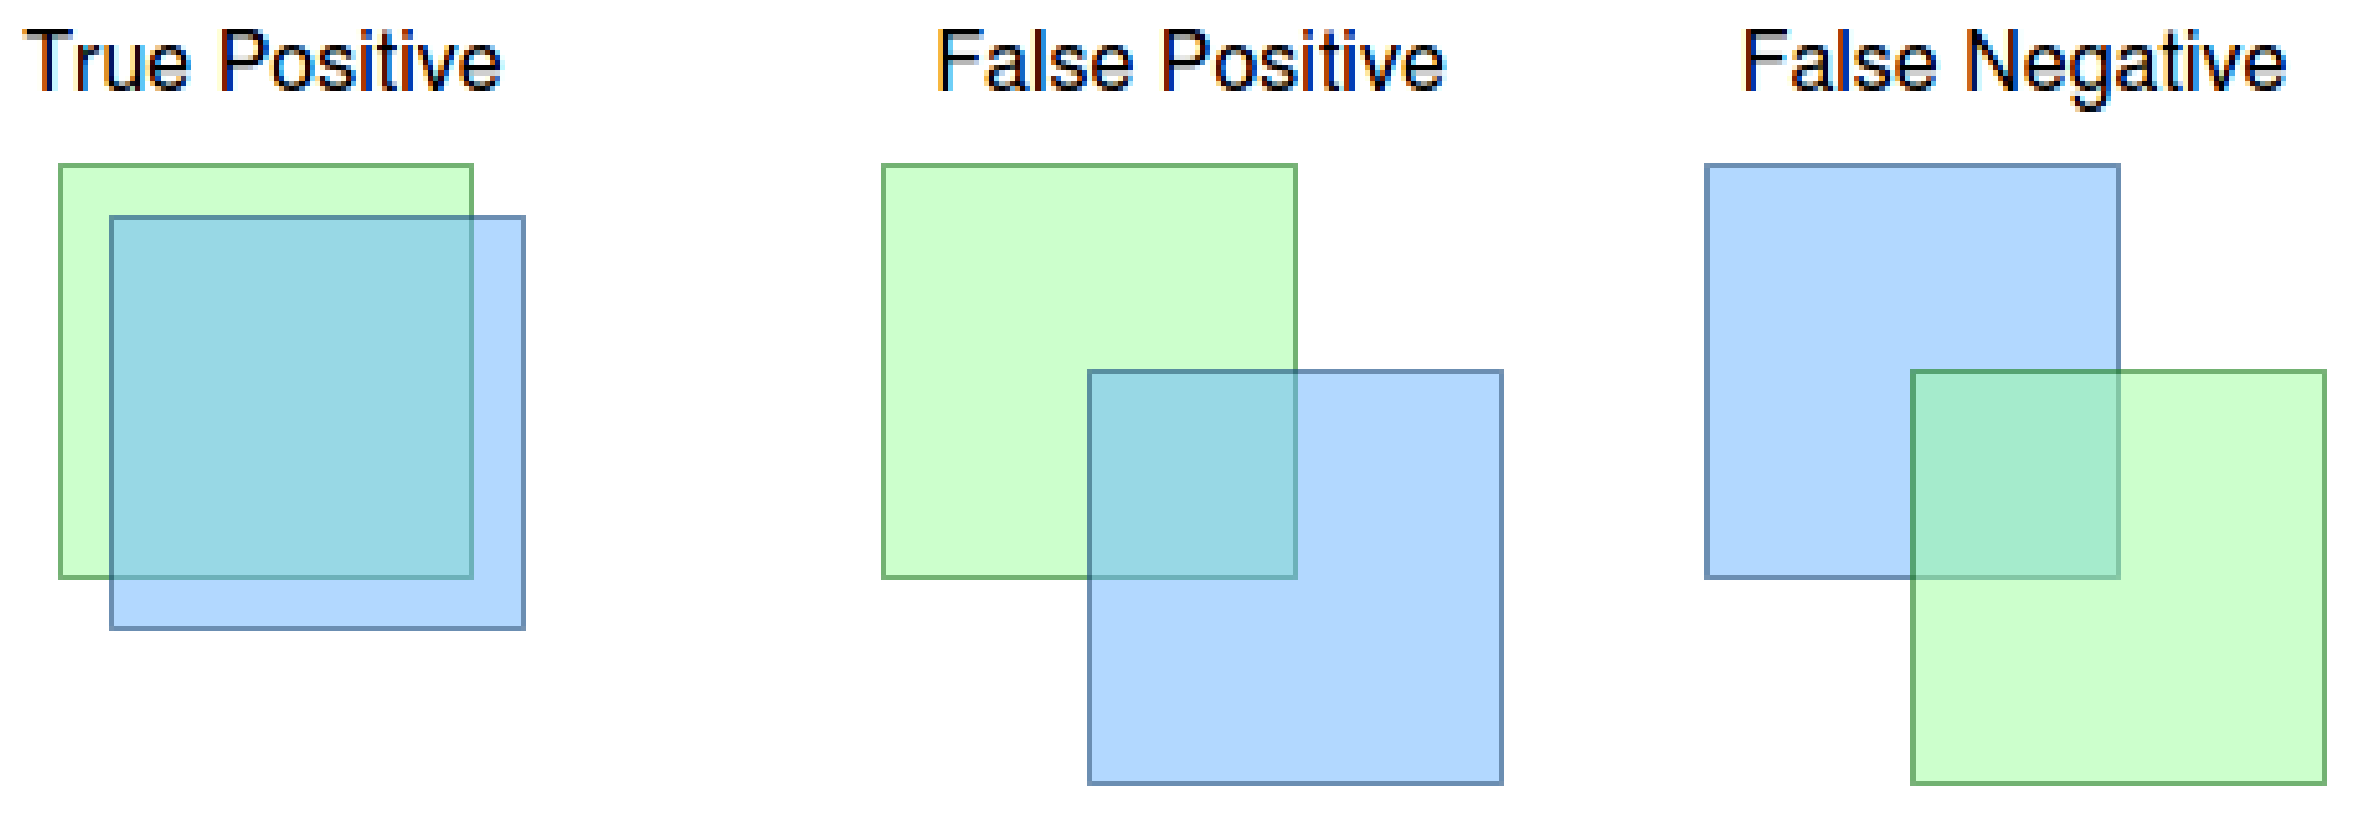
\includegraphics[width=0.5\textwidth]{obrazky-figures/iou_metric.png}
	\caption[Druhy detekce: skutečně pozitivní, falešně pozitivní a falešně negativní.]{Druhy detekce: skutečně pozitivní, falešně pozitivní a falešně negativní.\footnotemark}
	\label{fig:iou_metriky}
\end{figure}
\footnotetext{Obrázek pochází z~\cite{Bilik2021}, Obrázek 4.}

\textbf{Přesnost} (Precision, P) vyjadřuje, jaká část všech provedených detekcí byla správná, tedy kolik z~predikovaných objektů skutečně existuje.

\[P = \frac{TP}{TP + FP}\]

\textbf{Úplnost} (Recall, R) vyjadřuje, jaká část všech reálných objektů v~obraze byla detekována, tedy jak moc je model schopen zachytit vše, co existuje.

\[R = \frac{TP}{TP + FN}\]

Tyto dvě metriky jsou vzájemně provázány: se zvyšujícím se prahem spolehlivosti (confidence threshold) roste přesnost detekce, zatímco úplnost klesá, protože model odmítá méně jisté predikce. Naopak snížení prahu vede k~vyšší úplnosti za cenu nárůstu FP detekcí. Práh spolehlivosti představuje minimální hodnotu pravděpodobnosti (confidence score), kterou model přiřazuje detekovanému objektu. Pouze detekce s~hodnotou vyšší než tento práh jsou považovány za platné a zahrnují se do výsledku \cite{Padilla2020}. Proto hodnota prahu závisí na konkrétním použití, například v~kontextu detekce kleštíka je vhodné preferovat vyšší úplnost (tedy nižší práh spolehlivosti), jelikož přehlédnutí přítomnosti roztoče představuje větší riziko než~falešný poplach \cite{Bilik2021}.

\textbf{F1 skóre} je harmonickým průměrem přesnosti a úplnosti a poskytuje jednu souhrnnou hodnotu, která nabízí komplexnější vhled do vyhodnocení výkonu modelu.

\[F_1 = 2 \cdot \frac{P \cdot R}{P + R}\]

Harmonický průměr (na rozdíl od aritmetického) penalizuje situace, kdy je jedna z~hodnot výrazně nižší. F1 skóre je zvláště užitečné pro srovnání modelů při daném pevném prahu spolehlivosti a je standardní metrikou v~aplikacích detekce včel a Varroa, kde studie typicky reportují F1 při IoU@0.5 \cite{Bilik2021}.

\textbf{Průměrná přesnost} (Average Precision, AP) agreguje výkon modelu přes celý rozsah hodnot prahu spolehlivosti. Počítá se jako plocha pod křivkou přesnosti a úplnosti (Precision–Recall curve). Každý bod na křivce odpovídá jedné hodnotě prahu spolehlivosti.

\textbf{Střední průměrná přesnost} (mean Average Precision, mAP) je průměrem AP přes všechny třídy objektů v~datové sadě.

\[mAP = \frac{1}{N} \sum_{i = 1}^N AP_i\]

kde \(N\) představuje počet tříd. Hodnota mAP@0.5 představuje mAP při pevném IoU prahu~0,5 a je nejčastěji využívanou metrikou v~literatuře zaměřené na monitorování včelstev \cite{Bilik2021}. 

Pro nasazení na edge zařízeních jsou vedle přesnostních metrik klíčové také metriky výpočetní efektivity. \textbf{Snímková frekvence} (Frames Per Second, FPS) udává, kolik snímků je model schopen zpracovat za sekundu, a tím určuje, zda je aplikace schopna real-time provozu dosáhnout. \textbf{Latence} (inference time) označuje dobu potřebnou ke zpracování jednoho snímku v~milisekundách.

\chapter{Zhodnocení současného stavu a návrh řešení} \label{sec:zhodnoceni_navrh}
Předchozí kapitoly ukázaly, že oblast monitorování včelstev disponuje jak rozvinutým komerčním trhem, tak aktivní akademickou základnou. Cílem kapitoly je tato dvě prostředí kriticky porovnat, identifikovat potřeby, které dosud nebyly uspokojeny, a na základě tohoto rozboru formulovat cíle a návrh vlastního řešení.

Komerční produkty jsou obecně na vysoké úrovni z~hlediska hardwarového zpracování i uživatelského rozhraní. Váhy od VeluBee, BeeSage nebo BeeHiveMonitoring jsou robustní, snadno instalovatelné a nabízejí přehledné webové nebo mobilní aplikace s~detekcí základních událostí, jako jsou rojení nebo loupež. Tyto vlastnosti jsou pro běžného včelaře zásadní a je vhodné je zohlednit i ve vlastním návrhu. 

Přesto mají téměř všechna komerční řešení dva společné nedostatky. Prvním je absence automatické vizuální analýzy česna -- mechanické čítače včel, například od BeeHiveMonitoring, sice umožňují sledovat počet průchodů, avšak nedokáží jednotlivé jedince rozlišit ani klasifikovat. Včelař tak nemůže být automaticky upozorněn například na přítomnost predátora. Druhým nedostatkem je uzavřenost těchto systémů: zdrojový kód ani použité analytické metody nejsou veřejně dostupné. Včelař je tak závislý na konkrétním výrobci a jeho cloudové infrastruktuře, často i na placeném předplatném. Oba tyto nedostatky představují příležitost, kterou se tato práce snaží využít.

Z~akademické sféry jsou pro tuto práci relevantní zejména dva projekty. Systém Beemon \cite{Beemon2021} z~Appalachian State University kombinuje senzorový monitoring (teplota, vlhkost, hmotnost) s~audiovizuálními záznamy z~česna na platformě Raspberry Pi 4 a zasílá upozornění prostřednictvím IoT platformy ThingsBoard. Klíčovým omezením je však způsob zpracování obrazu: místo moderních detektorů objektů (např. YOLO nebo SSD) autoři segmentují včely na základě jejich obrysů, což je přístup citlivý na změny osvětlení a překryvy jedinců.

Druhým relevantním projektem je práce Nevláčila, Bilíka a Horáka z~VUT v~Brně \cite{Nevlacil2023}, zaměřená na detekci roztočů \textit{Varroa destructor} pomocí počítačového vidění v~kombinaci se senzorovým monitoringem. Na rozdíl od~systému Beemon využívá moderní přístup k~detekci objektů a přenáší data protokolem MQTT, což z~něj činí bližší referenci pro tuto práci. Systém je postaven na platformě Raspberry Pi a vyznačuje se modulární architekturou a využitím standardních IoT technologií. Zároveň však vyžaduje relativně výkonný hardware a stabilní komunikační infrastrukturu, což může být limitující při nasazení v~odlehlých lokalitách.

Oba systémy navíc ukazují, že platforma Raspberry Pi je schopna zvládat náročnější real-time úlohy, jako je zpracování videa, a že 3D tisk představuje dostupný a flexibilní způsob výroby mechanických částí na míru.

\section{Srovnání použitých technologií a jejich omezení}
Z~hlediska použitých technologií lze současná řešení rozdělit do tří základních kategorií podle způsobu získávání informací o~stavu včelstva. 

Základ většiny systémů tvoří senzorový monitoring fyzikálních veličin -- zejména hmotnosti úlu, teploty a vlhkosti. Výhodou je relativní jednoduchost, nízká energetická náročnost a vysoká spolehlivost dlouhodobého provozu. Nevýhodou je nepřímý charakter informací. Například pokles hmotnosti signalizuje možné rojení, ale nedokáže jej potvrdit ani odlišit od jiných příčin.

Druhou kategorii tvoří akustické systémy analyzující zvuk uvnitř úlu. Umožňují zachytit změny v~chování včelstva dříve, než  se projeví v senzorových datech, například při přípravě na rojení. Jejich nevýhodou je vyšší citlivost na šum prostředí a složitější interpretace signálu vyžadující specializované metody zpracování. 

Nejpokročilejší přístup představují systémy využívající počítačové vidění. Na rozdíl od senzorového monitoringu umožňují přímo analyzovat dění na česně -- detekovat a klasifikovat jedince, sledovat směr jejich pohybu nebo identifikovat predátory. Právě tato schopnost představuje informační hodnotu, kterou senzory ani akustické systémy nedokáží nahradit. Nevýhodou je výrazně vyšší výpočetní náročnost, potřeba kvalitního a stabilního osvětlení a nutnost robustních modelů schopných pracovat v~proměnlivých venkovních podmínkách.

Z~pohledu hardwaru a komunikačních technologií je patrný rozdíl mezi komerčními a akademickými řešeními. Komerční produkty staví na energeticky úsporných mikrokontrolérech a specializovaných deskách plošných spojů (PCB) optimalizovaných pro konkrétní aplikaci, přičemž komunikaci zajišťují mobilní sítě nebo nízkoenergetické protokoly umožňující vzdálený přístup k~datům. To přináší uživatelský komfort, avšak za cenu závislosti na výrobci a jeho infrastruktuře. Akademické projekty naopak preferují univerzální platformy jako Raspberry Pi, které usnadňují rychlé prototypování a implementaci pokročilých algoritmů, avšak za cenu vyšší spotřeby energie.

Z~tohoto srovnání vyplývají dvě klíčová zjištění pro návrh vlastního řešení. Za prvé, žádná z~kategorií sama o~sobě neposkytuje úplný obraz o~stavu včelstva -- teprve kombinace senzorového monitoringu s~počítačovým viděním přináší jak dlouhodobý kontextový pohled, tak schopnost identifikovat konkrétní události na česně. Za druhé, výhody komerčních řešení (robustnost, jednoduchost nasazení) a akademických projektů (otevřenost, flexibilita) se vzájemně doplňují a jejich propojení představuje přirozenou motivaci pro vlastní návrh popsaný v~následujících sekcích.

\section{Navázání na předchozí práci} \label{sec:navazani}
Tato práce navazuje na bakalářskou práci Bc. Kataríny Chovancové \cite{Chovancova2025}, která se zabývala návrhem a realizací kamerového systému pro monitorování dění na letáku úlu. Základ systému tvoří jednodeskový počítač Raspberry Pi 5, pro analýzu obrazu je využíván model počítačového vidění YOLOv8n, schopný detekovat tři třídy: včelu, včelí matku a vosu. Naměřená data jsou přenášena prostřednictvím mobilního datového připojení na IoT platformu ThingsBoard, napájení zajišťuje baterie se solárním panelem. 

Přestože uvedený systém představuje funkční základ pro vizuální monitorování česna, má klíčové omezení. Zaměřuje se výhradně na obrazová data z~česna a neposkytuje žádné informace o~fyzikálním stavu včelstva uvnitř úlu. 

Cílem navrhovaného řešení je toto omezení překonat a vytvořit komplexnější monitorovací řešení kombinující více zdrojů informací. Konkrétně jde o~doplnění senzorového modulu měřícího hmotnost úlu, teplotu a vlhkost, které umožňují dlouhodobé sledování stavu včelstva. Součástí řešení je rovněž integrace kamerového systému z~předchozí práce do nově navržené architektury. 

\begin{figure}[H]
    \centering
    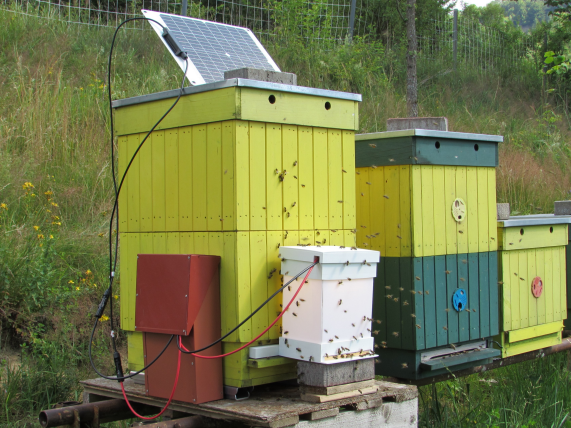
\includegraphics[width=0.7\textwidth]{obrazky-figures/vysledek_chovancova.png}
    \caption{Výsledná podoba zařízení Bc. Kataríny Chovancové \cite{Chovancova2025}.}
    \label{fig:vysledek_chovancova}
\end{figure}

\section{Návrh systému a výběr materiálů}
Navrhovaný systém pro monitorování včelstev se skládá ze dvou vzájemně nezávislých, ale komplementárních modulů: senzorového pro měření hmotnosti, teploty a vlhkosti a kamerového pro vizuální analýzu česna. Oba moduly jsou navrženy jako samostatně funkční celky, které lze nasadit nezávisle nebo kombinovat. Tato modularita je vědomou volbou oproti komerčním řešením, kde bývají senzory vázány na proprietární hub nebo cloudovou infrastrukturu konkrétního výrobce. Celý systém je open-source a veškerý kód i návrh konstrukce jsou veřejně dostupné v repozitáři na platformě GitHub\,\footnote{\url{https://github.com/e-kreme/Robotic-Beekeeper}}.

Požadavky na systém vycházejí z~analýzy komerčních řešení, odborné literatury a praktických včelařských zkušeností:

\begin{itemize}
    \item zajištění celoročního provozu v~proměnlivých venkovních podmínkách
    \item dostatečná přesnost měření umožňující detekci relevantních událostí ve včelstvu (např. snůška, rojení, úhyn)
    \item využití cenově dostupných komponent s~ohledem na výslednou cenu zařízení
    \item jednoduchá instalace bez nutnosti zásadních zásahů do konstrukce úlu
    \item průběžný sběr a zpracování dat s~přehlednou vizualizací, včetně možnosti lokálního zobrazení přímo na zařízení
    \item minimalizace vlivu systému na přirozené chování včelstva
\end{itemize}

\subsection*{Návrh architektury systému}
Architektura systému odráží přirozené rozdělení rolí jednotlivých komponent. Senzorový modul postavený na mikrokontroléru ESP32-S3 průběžně měří fyzikální veličiny charakterizující stav včelstva (podrobněji viz sekce \ref{sec:veliciny}) -- konkrétně hmotnost úlu, venkovní teplotu a vnitřní podmínky v~úlu (teplotu, vlhkost a tlak).

Data jsou průběžně zpracovávána a následně přenášena prostřednictvím bezdrátové komunikace do vzdáleného úložiště pro další analýzu a vizualizaci. Data jsou odesílána prostřednictvím protokolu MQTT, který je pro IoT aplikace tohoto typu standardní volbou \cite{Beemon2021}, \cite{Nevlacil2023}, \cite{Chovancova2025}, na Raspberry Pi 4 sloužící jako centrální úložiště. Kamerový modul s~Raspberry Pi 5 zpracovává obrazová data z~česna lokálně a výsledky vizuální analýzy jsou integrovány se senzorovými záznamy. Vzdálený přístup k~datům je zajištěn prostřednictvím VPN sítě Tailscale. Napájení senzorového modulu zajišťuje baterie v~kombinaci se solárním panelem, kamerový modul je napájen ze sítě.

Z~hlediska softwaru je firmware senzorového modulu vyvíjen v~prostředí Arduino IDE, které poskytuje přímou podporu pro použité senzory a komunikační protokoly. Zpracování a analýza dat probíhá v~jazyce Python. Pro vizualizaci časových průběhů měřených veličin je využita platforma Grafana, která umožňuje přehledné zobrazení dat a jejich vzdálenou správu.

\subsection*{Návrh konstrukce úlové váhy}
Základním prvkem senzorového modulu je konstrukce úlové váhy určená pro dlouhodobé a spolehlivé měření hmotnosti úlu v~reálných venkovních podmínkách. Klíčovým konstrukčním rozhodnutím je volba počtu a rozmístění váhových senzorů, přičemž v~praxi se lze setkat se třemi přístupy.

Nejjednodušší je hranový způsob vážení, kdy je jedna hrana úlu podložena váhou a naměřená hodnota se zdvojí za předpokladu symetrického rozložení hmotnosti úlu. Tento přístup je cenově nenáročný, avšak nepřesný -- rozložení hmotnosti v~úlu se v~průběhu roku mění v~závislosti na tvorbě a spotřebě zásob. Druhým přístupem jsou váhy se dvěma nebo čtyřmi senzorovými buňkami, například od BeeSage nebo BeeHiveMonitoring, které nezávisí na centrickém umístění zátěže. Nevýhodou je vyšší cena a náročnější kalibrace, protože každá buňka musí být kalibrována zvlášť.

Pro tuto práci jsem zvolila třetí přístup -- jedinou centrální váhovou buňku, stejně jako u~systému VeluBee. Úl je uložen na rámové nosné konstrukci a váhový senzor je umístěn mezi dvěma mechanicky oddělenými částmi rámu, čímž je zatížení přenášeno přímo na měřicí prvek. Toto uspořádání zachovává dostatečnou mechanickou stabilitu a zároveň zjednodušuje kalibraci.

\begin{figure}[H]
    \centering
    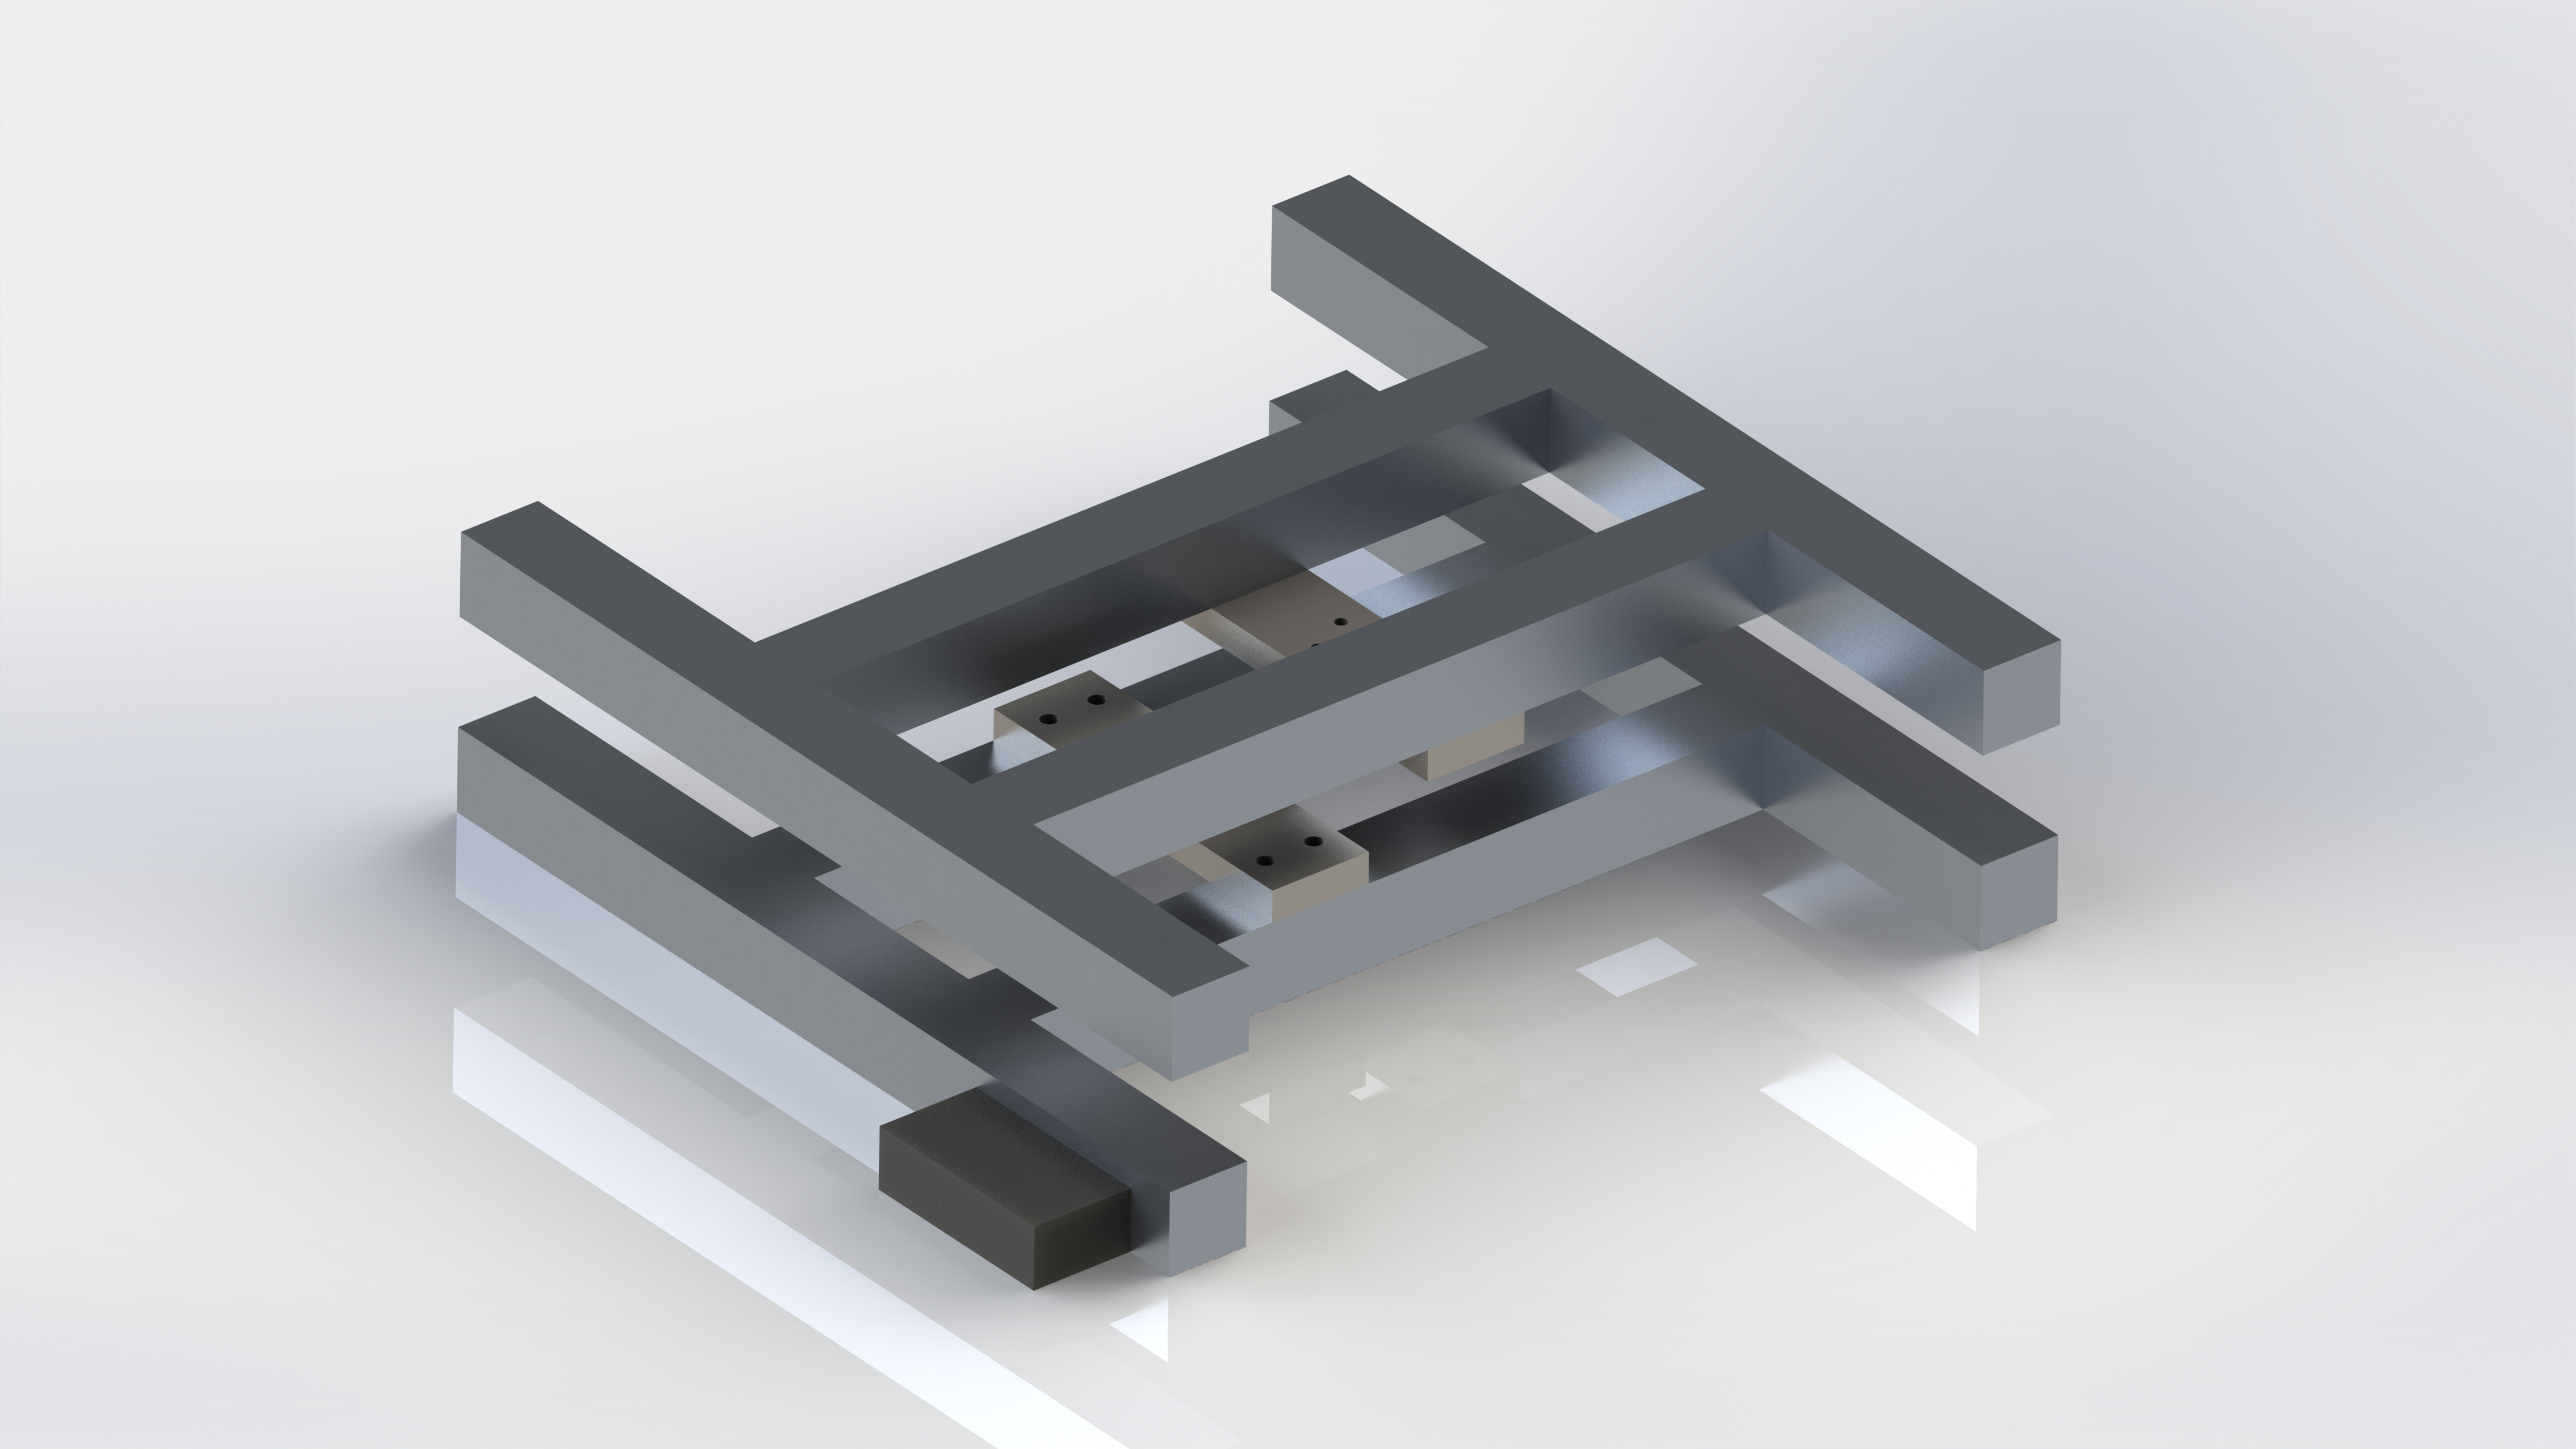
\includegraphics[width=0.7\textwidth]{obrazky-figures/navrh_solidworks.JPG}
    \caption{3D model konstrukce úlové váhy.}
    \label{fig:navrh_solidworks}
\end{figure}

Konstrukce byla navržena v~prostředí SolidWorks (viz obrázek \ref{fig:navrh_solidworks}) a přizpůsobena rozměrům domácího úlu 46 $\times$ 46 cm. Pro ověření mechanické odolnosti byla v~prostředí ANSYS Workbench 2025 R2 provedena simulace zatížení 100 kg (viz obrázek \ref{fig:simulace_zatizeni}). Maximální celková deformace dosáhla přibližně $1{,}4 \times 10^{-4}$ m (0,14 mm) na okrajích horní části konstrukce, přičemž tato hodnota je vzhledem k~rozměrům konstrukce zanedbatelná a na přesnost měření nemá vliv. Simulace neodhalila žádná kritická místa ohrožující mechanickou integritu systému.

\begin{figure}[H]
    \centering
    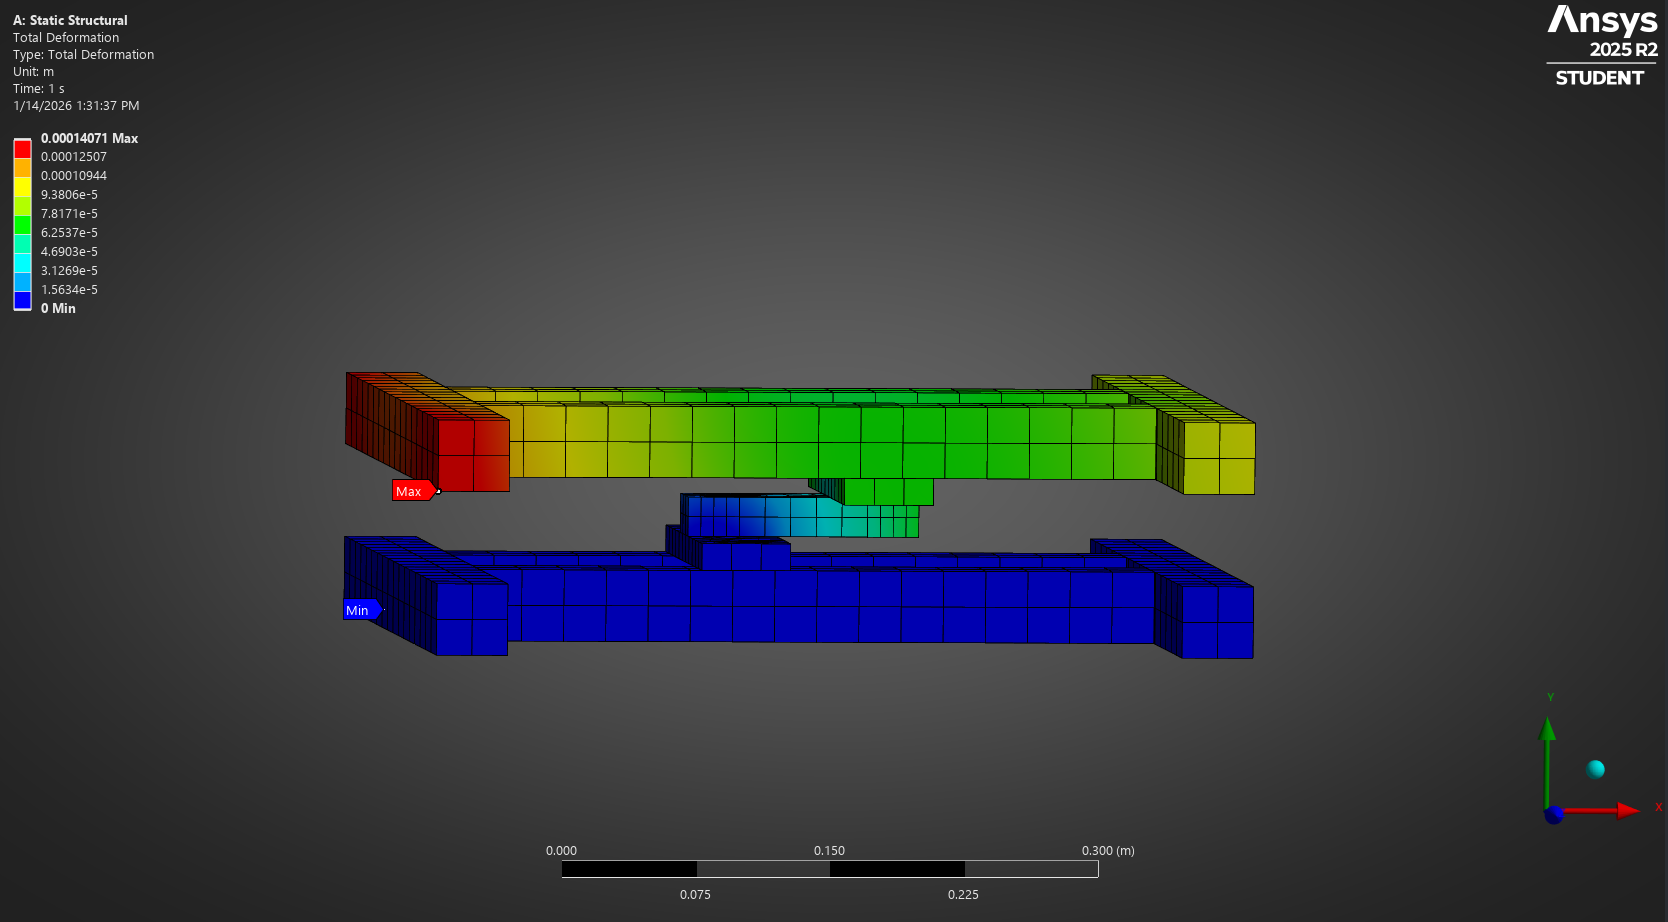
\includegraphics[width=0.7\textwidth]{obrazky-figures/simulace_zatizeni.png}
    \caption{Simulace zatížení vytvořeného modelu konstrukce hmotností 100 kg.}
    \label{fig:simulace_zatizeni}
\end{figure}

\subsection*{Výběr materiálu konstrukce}
Jako konstrukční materiál jsem zvolila standardizované hliníkové profily, které představují vhodný kompromis mezi hmotností, pevností a odolností vůči vnějším vlivům. Klíčovou vlastností je vysoká odolnost hliníku vůči korozi, a to i při mechanickém poškození povrchu, což je zásadní pro dlouhodobý provoz ve venkovním prostředí s~proměnlivou vlhkostí a teplotou. Ve srovnání s~ocelí má hliník nižší modul pružnosti, avšak jak dokládá výše uvedená simulace, výsledné deformace jsou při navržených rozměrech zcela zanedbatelné. Použití standardizovaných profilů navíc umožňuje modulární konstrukci snadno přizpůsobitelnou různým typům úlů nebo budoucím rozšířením systému.

\subsection*{Návrh kamerového modulu pro monitorování letáku}
Kamerový modul slouží k~vizuálnímu monitorování česna a vychází z~konstrukce navržené v~předchozí bakalářské práci \cite{Chovancova2025}, kterou jsem upravila pro rozměry domácího úlu. 3D model byl vytvořen v~prostředí SolidWorks (viz obrázek \ref{fig:3d_model_krabicky}).

\begin{figure}[H]
	\centering
    \begin{subfigure}[b]{0.5\textwidth}
        \centering
        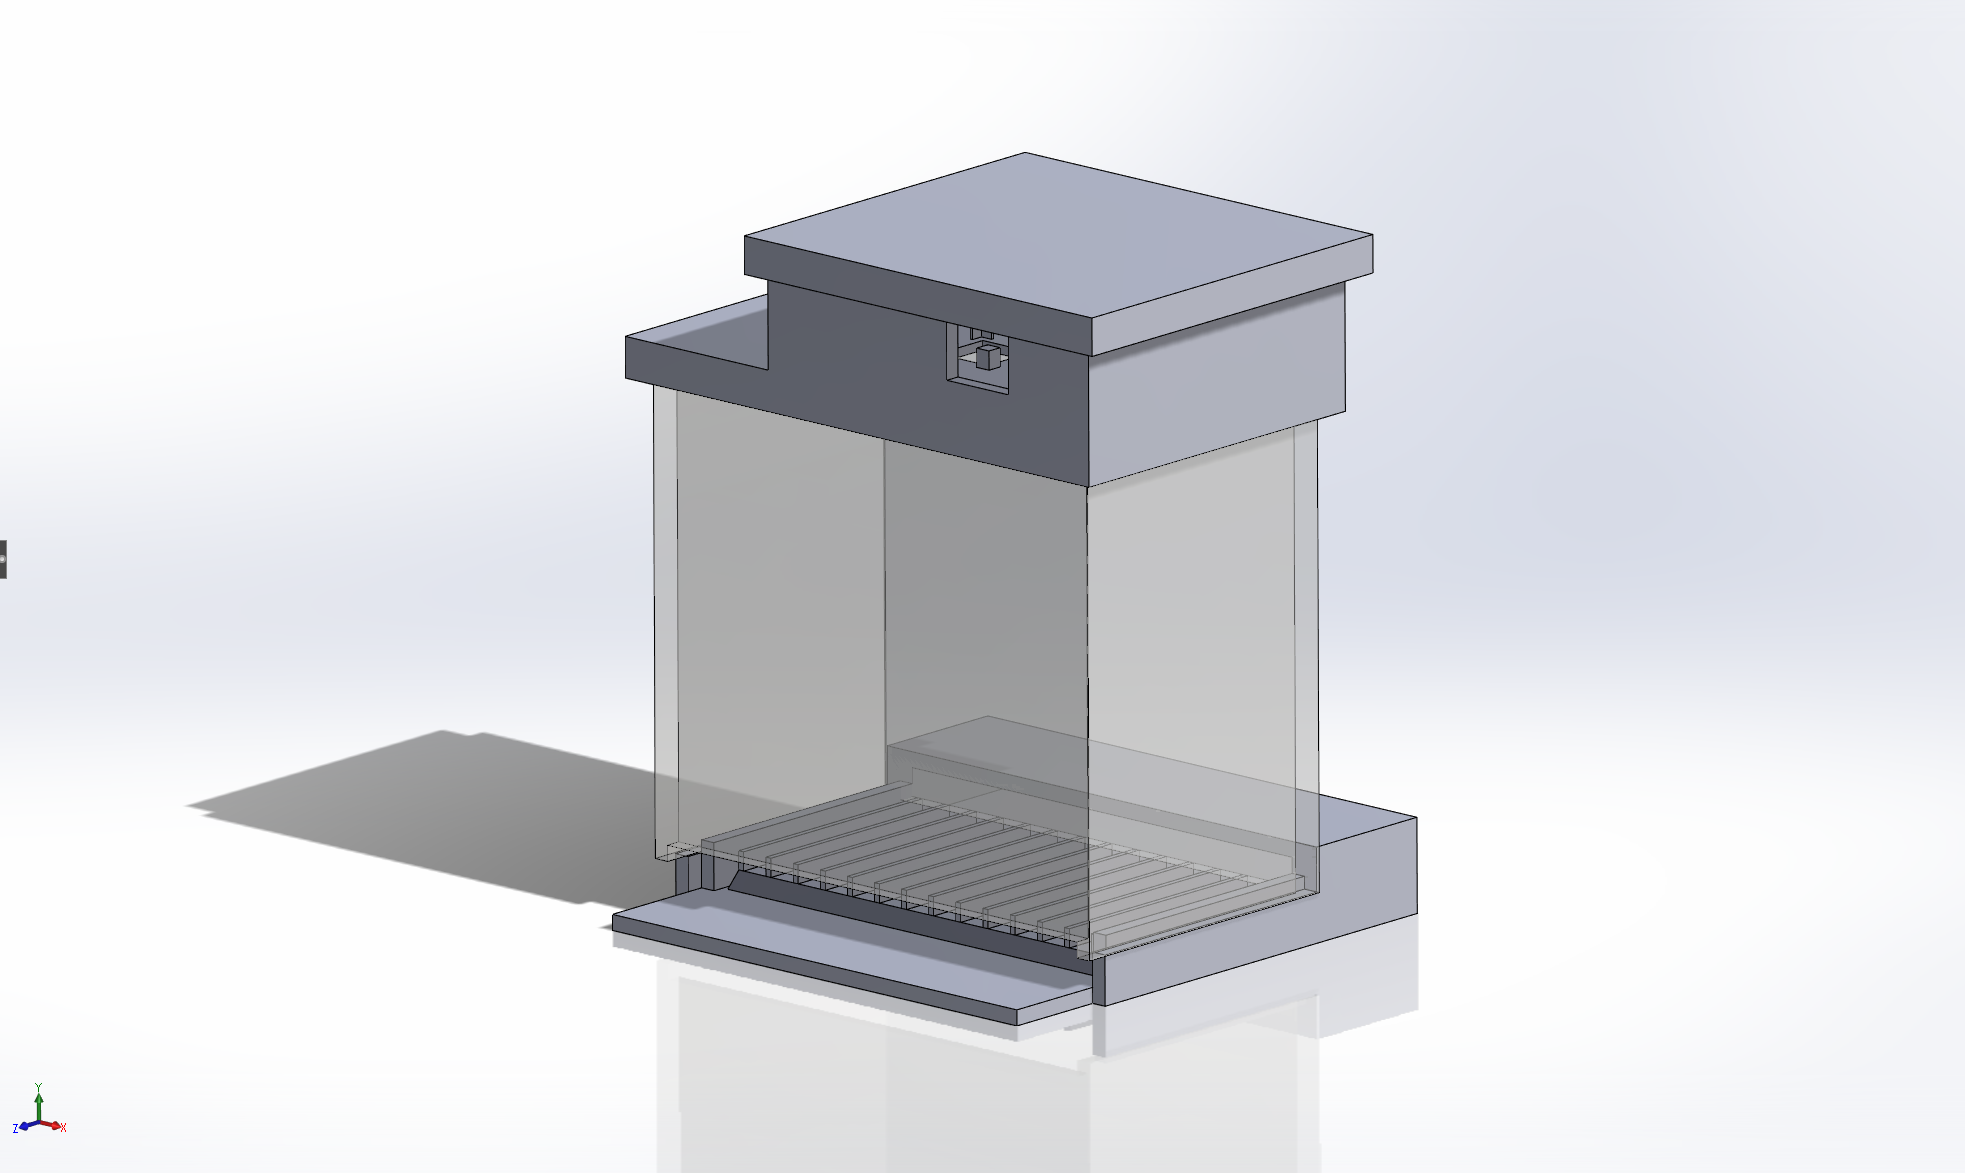
\includegraphics[width=\textwidth]{obrazky-figures/3d_model_bocni_pohled.png}
        \label{fig:3d_model_bocni_pohled}
    \end{subfigure}\hfill\begin{subfigure}[b]{0.5\textwidth}
        \centering
        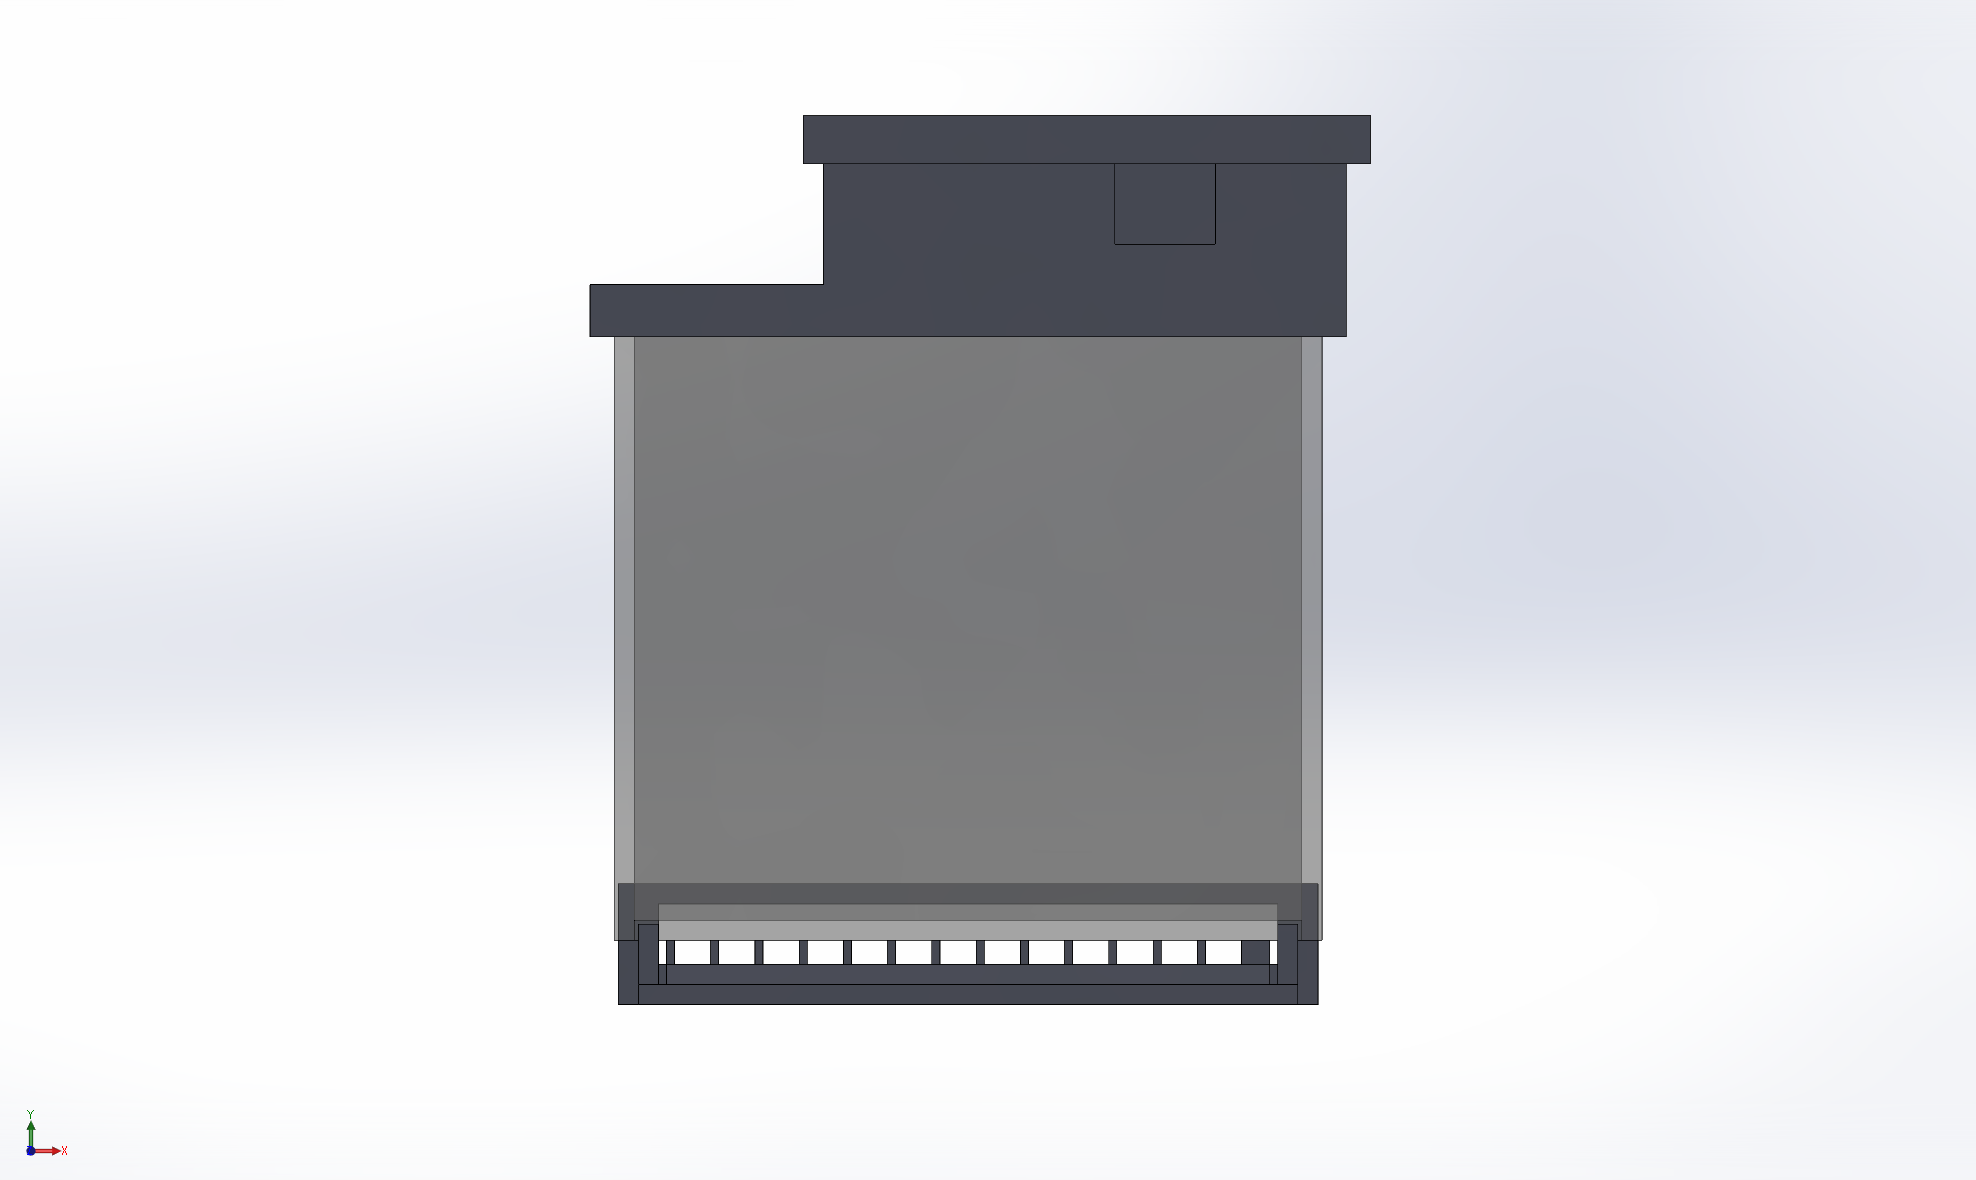
\includegraphics[width=\textwidth]{obrazky-figures/3d_model_predni_pohled.png}
        \label{fig:3d_model_predni_pohled}
    \end{subfigure}
	
	\caption{3D model krabičky pro kamerový modul, přední a boční pohled.}
	\label{fig:3d_model_krabicky}
\end{figure}

Modul je navržen jako samostatný celek, který se umisťuje před česno úlu. Nejvýznamnější úpravou oproti původní konstrukci je zavedení průchodových tunelů, kterými včely vstupují a vystupují z~úlu. Tunely usměrňují pohyb včel do definovaných trajektorií, čímž snižují vzájemné překryvy jedinců -- častý problém při analýze obrazu volného prostoru před česnem -- a zjednodušují detekci a sledování směru pohybu. Rozměry průchodů jsou navrženy tak, aby včelám nepůsobily stres a poskytovaly dostatečný prostor i pro větší jedince kolonie, například pro včelí matku nebo trubce. Modul je z~výrobních a praktických důvodů rozdělen do několika samostatných částí (viz obrázek \ref{fig:3d_model_rozlozeny}), což usnadňuje manipulaci i případné budoucí úpravy.

\begin{figure}[H]
    \centering
    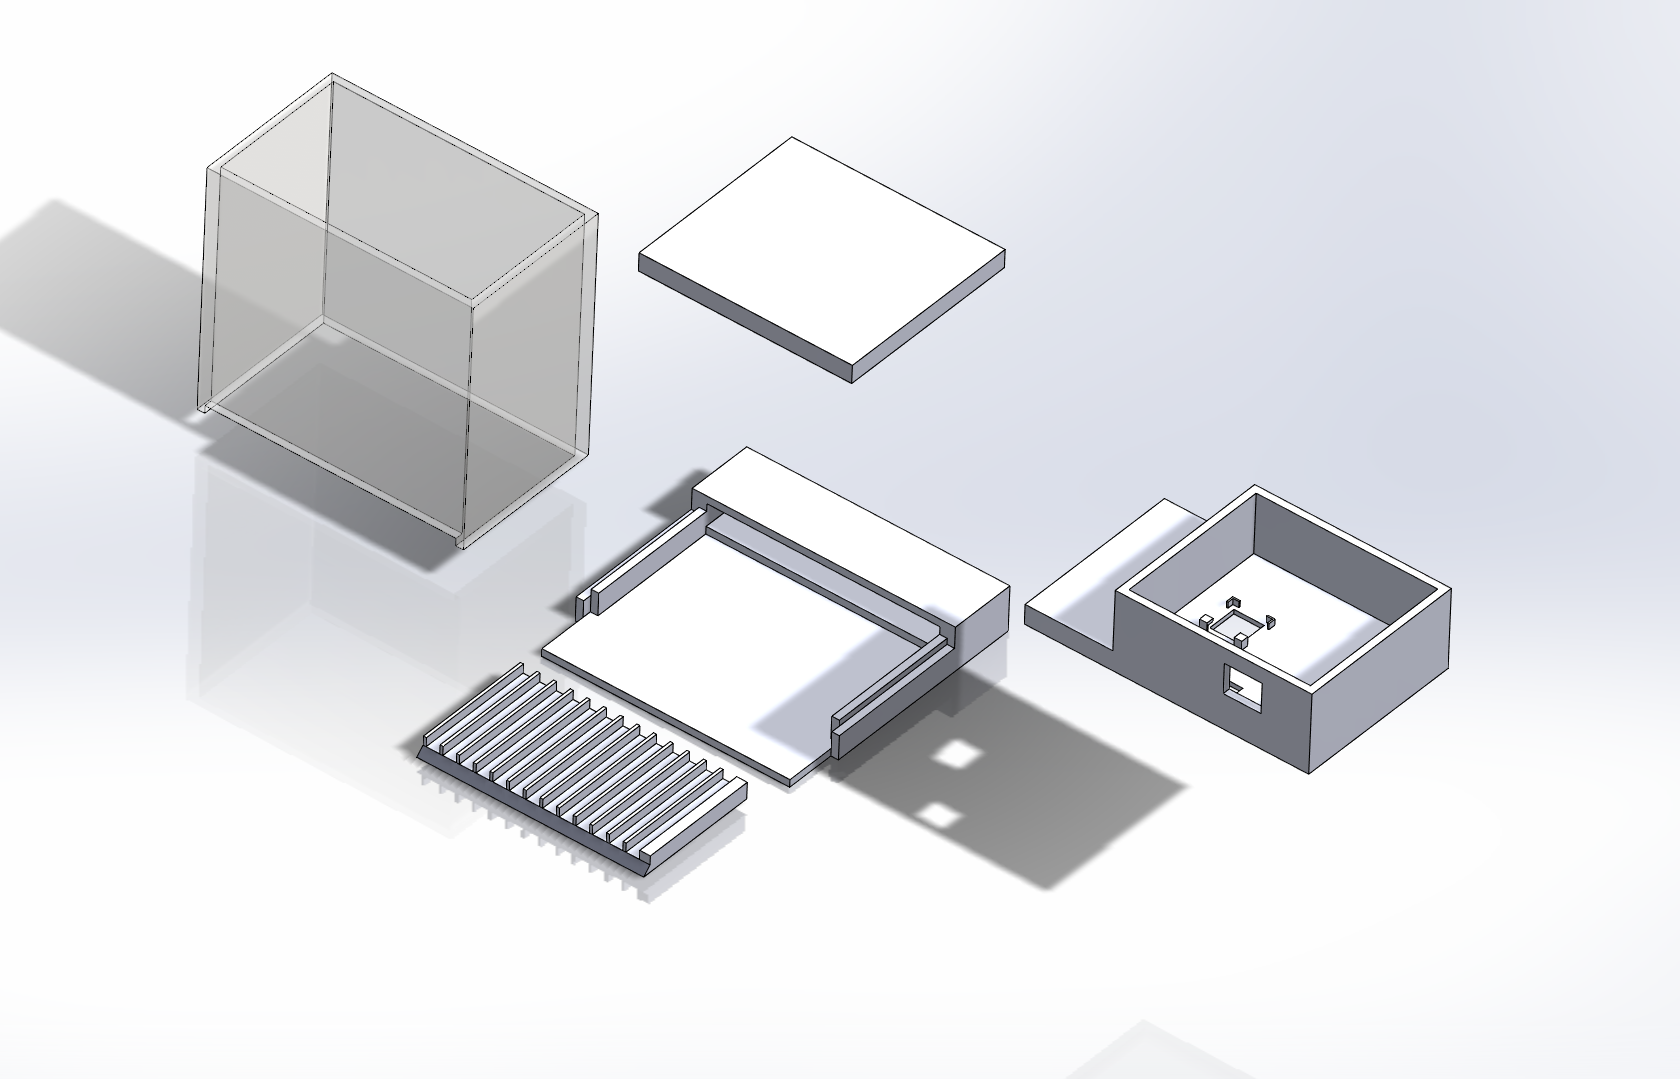
\includegraphics[width=0.7\textwidth]{obrazky-figures/3d_model_rozlozeny.png}
    \caption{3D model krabičky pro kamerový modul, rozložený na jednotlivé části.}
    \label{fig:3d_model_rozlozeny}
\end{figure}

\section{Výběr hardwaru a technologií}
Pro realizaci navrženého systému bylo nutné zvolit vhodné hardwarové komponenty s~ohledem na požadavky definované v~předchozí sekci, zejména na nízkou energetickou náročnost, spolehlivost v~dlouhodobém provozu a cenovou dostupnost. Tabulka \ref{tab:prehled_cen_komponent} obsahuje ceny veškerých použitých komponent a dalšího příslušenství.

\subsection*{Senzorový modul}
Řídicí jednotkou senzorového modulu je mikrokontrolér ESP32-S3 ve variantě LilyGO TTGO T-Display-S3. Čip disponuje dvoujádrovým procesorem Xtensa LX7 s~taktem až 240 MHz, 16MB flash pamětí, 8MB PSRAM, Wi-Fi 802.11 b/g/n a Bluetooth 5.0. Klíčovými důvody volby jsou integrovaná Wi-Fi konektivita umožňující odesílání dat protokolem MQTT, dostatečný výpočetní výkon a široká dostupnost vývojových nástrojů a knihoven. Mikrokontrolér je napájen pomocí USB-C a podporuje i připojení lithiové baterie pomocí konektoru JST. Integrovaný displej pak umožňuje lokální zobrazení naměřených hodnot při~tradiční kontrole úlu bez nutnosti externího zařízení.

Pro měření hmotnosti jsem zvolila tenzometrický snímač GUANG CE YZC-1B s~maximálním zatížením 100 kg, který je dostačující pro předpokládaný rozsah hmotnosti úlu včetně zásob. Jedná se o~\textit{single-point load cell} z~hliníkové slitiny. Bezpečné přetížení činí 120\,\% a limitní přetížení 150\,\%, což je pro hmotnost úlu více než dostačující. Analogový signál snímače je zpracováván 24bitovým převodníkem HX711 navrženým přímo pro Wheatstoneovy můstkové snímače.

Venkovní teplota je měřena vodotěsnou verzí senzoru DS18B20 s~kabelem délky 1 m. Původně byl pořízen senzor DHT11, který však byl po praktickém testování nahrazen, protože jeho rozsah 0 až +50\,°C nestačí pro celoroční venkovní provoz. DS18B20 pokrývá rozsah $-55$ až $+125$\,°C. Vnitřní podmínky úlu (teplotu, vlhkost a tlak) měří senzor BME280 umístěný v~ochranném obalu chránícím jej před propolisem a voskem. Veškerá řídicí elektronika je uložena v~krabičce s~krytím IP66, které zajišťuje ochranu před prachem a silným proudem vody z~libovolného směru.

\subsection*{Napájení systému}
Napájecí soustava, převzatá od Bc. Chovancové \cite{Chovancova2025}, se skládá ze čtyř komponent. Zdrojem energie je flexibilní fotovoltaický panel 12 V/20 W propojený se systémem kabelem H1Z2Z2-K certifikovaným pro venkovní solární instalace. Regulaci nabíjení a ochranu baterie před přebitím a hlubokým vybitím zajišťuje PWM solární regulátor 12--24 V/10 A~s~USB výstupem, kompatibilní s~bateriemi Pb, LiFePO4 a Li-ion. Jako akumulátor slouží AGM GOOWEI ENERGY OT20-12 L1 (12 V, 20 Ah), který nahradil původní nefunkční akumulátor Green Cell se shodnými parametry.

\subsection*{Kamerový modul}
Výpočetní jádro kamerového modulu tvoří Raspberry Pi 5 s~4 GB RAM osazený čtyřjádrovým procesorem ARM Cortex-A76 s~taktem 2,4 GHz, uložený v~hliníkové krabičce s~aktivním chlazením. Pro snímání česna slouží Raspberry Pi Camera Module 3 se snímačem Sony IMX708 s~rozlišením 11,9 MP. Obě zařízení pocházejí z~předchozí práce \cite{Chovancova2025}. Doplňkovým prvkem je flexibilní LED neonový pásek TR-34N (bílý, 1,8 m, napájení USB) zajišťující konzistentní osvětlení sledované oblasti, které je důležitou podmínkou pro stabilní výkon modelu počítačového vidění.

\subsection*{Další komponenty}
Pro ukládání dat a jejich vizualizaci slouží Raspberry Pi 4 Model B s~2 GB RAM běžící jako lokální server. Kromě toho bylo využito standardních pomocných komponent -- propojovacích vodičů, napájecích kabelů a konektorů -- volených s~ohledem na spolehlivost spojení a odolnost vůči venkovnímu prostředí.

\newpage
 
\begin{table}[H]
    \centering
    \begin{tabular}{|m{10,5cm}|c|}
    \hline
    \textbf{Název komponenty} & \textbf{Cena} \\
    \hline
    \hline
    \multicolumn{2}{|l|}{\textbf{Senzorový modul}} \\
    \hline
    LilyGO TTGO T-Display-S3 ESP32-S3 WiFi Modul\,\footnotemark[1] & 768 Kč \\
    \hline
    GUANG CE YZC-1B Vážící senzor 100 kg\,\footnotemark[1] & 598 Kč\\
    \hline
    AD Převodník Modul 24-bit 2 kanály HX711\,\footnotemark[1] & 24 Kč \\
    \hline
    DS18B20 Digitální vodotěsné čidlo teploty 1 m\,\footnotemark[1] & 54 Kč \\
    \hline
    Senzor tlaku, teploty a vlhkosti BME280, 1 m\,\footnotemark[1] & 448 Kč \\
    \hline
    IP66 Vodotěsná Montážní Krabice\,\footnotemark[2] & 149 Kč \\
    \hline
    \textbf{Celková cena} & \textbf{2041 Kč} \\
    \hline
    \hline
    \multicolumn{2}{|l|}{\textbf{Napájení}} \\
    \hline
    Fotovoltaický solární panel 12V/20W, flexibilní, MC-4\,\footnotemark[3] & 19,33 € (471,46 Kč\,\footnotemark[4]) \\
    \hline
    Solární regulátor PWM 12-24 V/10 A+USB\,\footnotemark[3] & 11,16 € (272,19 Kč\,\footnotemark[4]) \\
    \hline
    Solární kabel H1Z2Z2-K, 4 mm2, konektory MC-4, 2 m\,\footnotemark[3] & 7,37 € (179,75 Kč\,\footnotemark[4]) \\
    \hline
    Bezúdržbový olověný akumulátor AGM OT20-12 L1, 12V, 20Ah\,\footnotemark[5] & 1189 Kč \\
    \hline
    \textbf{Celková cena} & \textbf{2112,40 Kč} \\
    \hline
    \hline
    \multicolumn{2}{|l|}{\textbf{Kamerový modul}} \\
    \hline
    Raspberry Pi 5 4 GB\,\footnotemark[6] & 65,50 € (1597,54 Kč\,\footnotemark[4]) \\
    \hline
    Raspberry Pi  Camera 3\,\footnotemark[7] & 28,08 € (684,87 Kč\,\footnotemark[4]) \\
    \hline
    Hliníková krabička pro Raspberry Pi 5 černá s ventilátory\,\footnotemark[6] & 11,40 € (278,05 Kč\,\footnotemark[4]) \\
    \hline
    LED neonový pásek TR-34N (bílý, 1,8 m, napájení USB)\,\footnotemark[8] & 116 Kč \\
    \hline
    \textbf{Celková cena} & \textbf{2676,46 Kč} \\
    \hline
    \hline
    \multicolumn{2}{|l|}{\textbf{Další komponenty}} \\
    \hline
    Kabelová vodotěsná průchodka, šedá\,\footnotemark[1] & 4 Kč \\
    \hline
    Dupont propojovací kabel 40žil F-F (10cm)\,\footnotemark[1] & 38 Kč \\
    \hline
    LaskaKit Sada 1000 rezistorů, 34 hodnot 1R -- 10M\,\footnotemark[1] & 298 Kč \\
    \hline
    Raspberry Pi 27W USB-C napájecí zdroj, EU, černý\,\footnotemark[6] & 11,30 € (275,61 Kč\,\footnotemark[4]) \\
    \hline
    Raspberry Pi 4 Model B -- 2GB RAM\,\footnotemark[7] & 46,82 € (1141,95 Kč\,\footnotemark[4]) \\
    \hline
    Raspberry Pi USB-C 5,1V3A napájecí zdroj, EU, černý\,\footnotemark[7] & 9,98 € (243,41 Kč\,\footnotemark[4]) \\
    \hline
    Puzdro na minipočítač JOY-IT Case pro RASPBERRY Pi 4 – Armor černé\,\footnotemark[9] & 11,59 € (282,68 Kč\,\footnotemark[4]) \\
    \hline
    Vention USB 2.0 to USB-C 3A Cable 0.5M Black\,\footnotemark[5] & 79 Kč \\
    \hline
    \textbf{Celková cena} & \textbf{2362,65 Kč} \\
    \hline
    \hline
    \textbf{Celková cena veškerých komponent} & \textbf{9192,51 Kč} \\
    \hline
    \end{tabular}
    \caption{Cena použitých hardwarových komponent a příslušenství.}
    \label{tab:prehled_cen_komponent}
\end{table}

\footnotetext[1]{Komponenta byla zakoupena na e-shopu: \url{https://www.laskakit.cz}}
\footnotetext[2]{Komponenta byla zakoupena na e-shopu: \url{https://www.chytrevypinace.cz}}
\footnotetext[3]{Komponenta pochází od \cite{Chovancova2025}, byla zakoupena na e-shopu \url{https://www.hadex.cz}}
\footnotetext[4]{Měnový kurz platný ke dni 5. května 2026}
\footnotetext[5]{Komponenta byla zakoupena na e-shopu: \url{https://www.alza.cz}}
\footnotetext[6]{Komponenta pochází od \cite{Chovancova2025}, byla zakoupena na e-shopu \url{https://www.elecom.sk}}
\footnotetext[7]{Komponenta pochází od \cite{Chovancova2025}, byla zakoupena na e-shopu \url{https://rpishop.cz}}
\footnotetext[8]{Komponenta byla zakoupena v kamenné prodejně UNI HOBBY Zlín}
\footnotetext[9]{Komponenta pochází od \cite{Chovancova2025}, byla zakoupena na e-shopu \url{https://www.alza.sk}}

\chapter{Implementace}
Tato kapitola popisuje realizaci navrženého systému od fyzické konstrukce zařízení přes přípravu dat a trénování modelů až po softwarové řešení a uživatelské rozhraní. Jednotlivé sekce sledují přirozenou posloupnost vývoje -- od hardwaru k~softwaru -- přičemž důraz je kladen na popis klíčových rozhodnutí a problémů, které bylo v~průběhu realizace nutné řešit.

\section{Konstrukce zařízení}

\subsection*{Úlová váha a senzorový modul}

\begin{figure}[H]
    \centering
    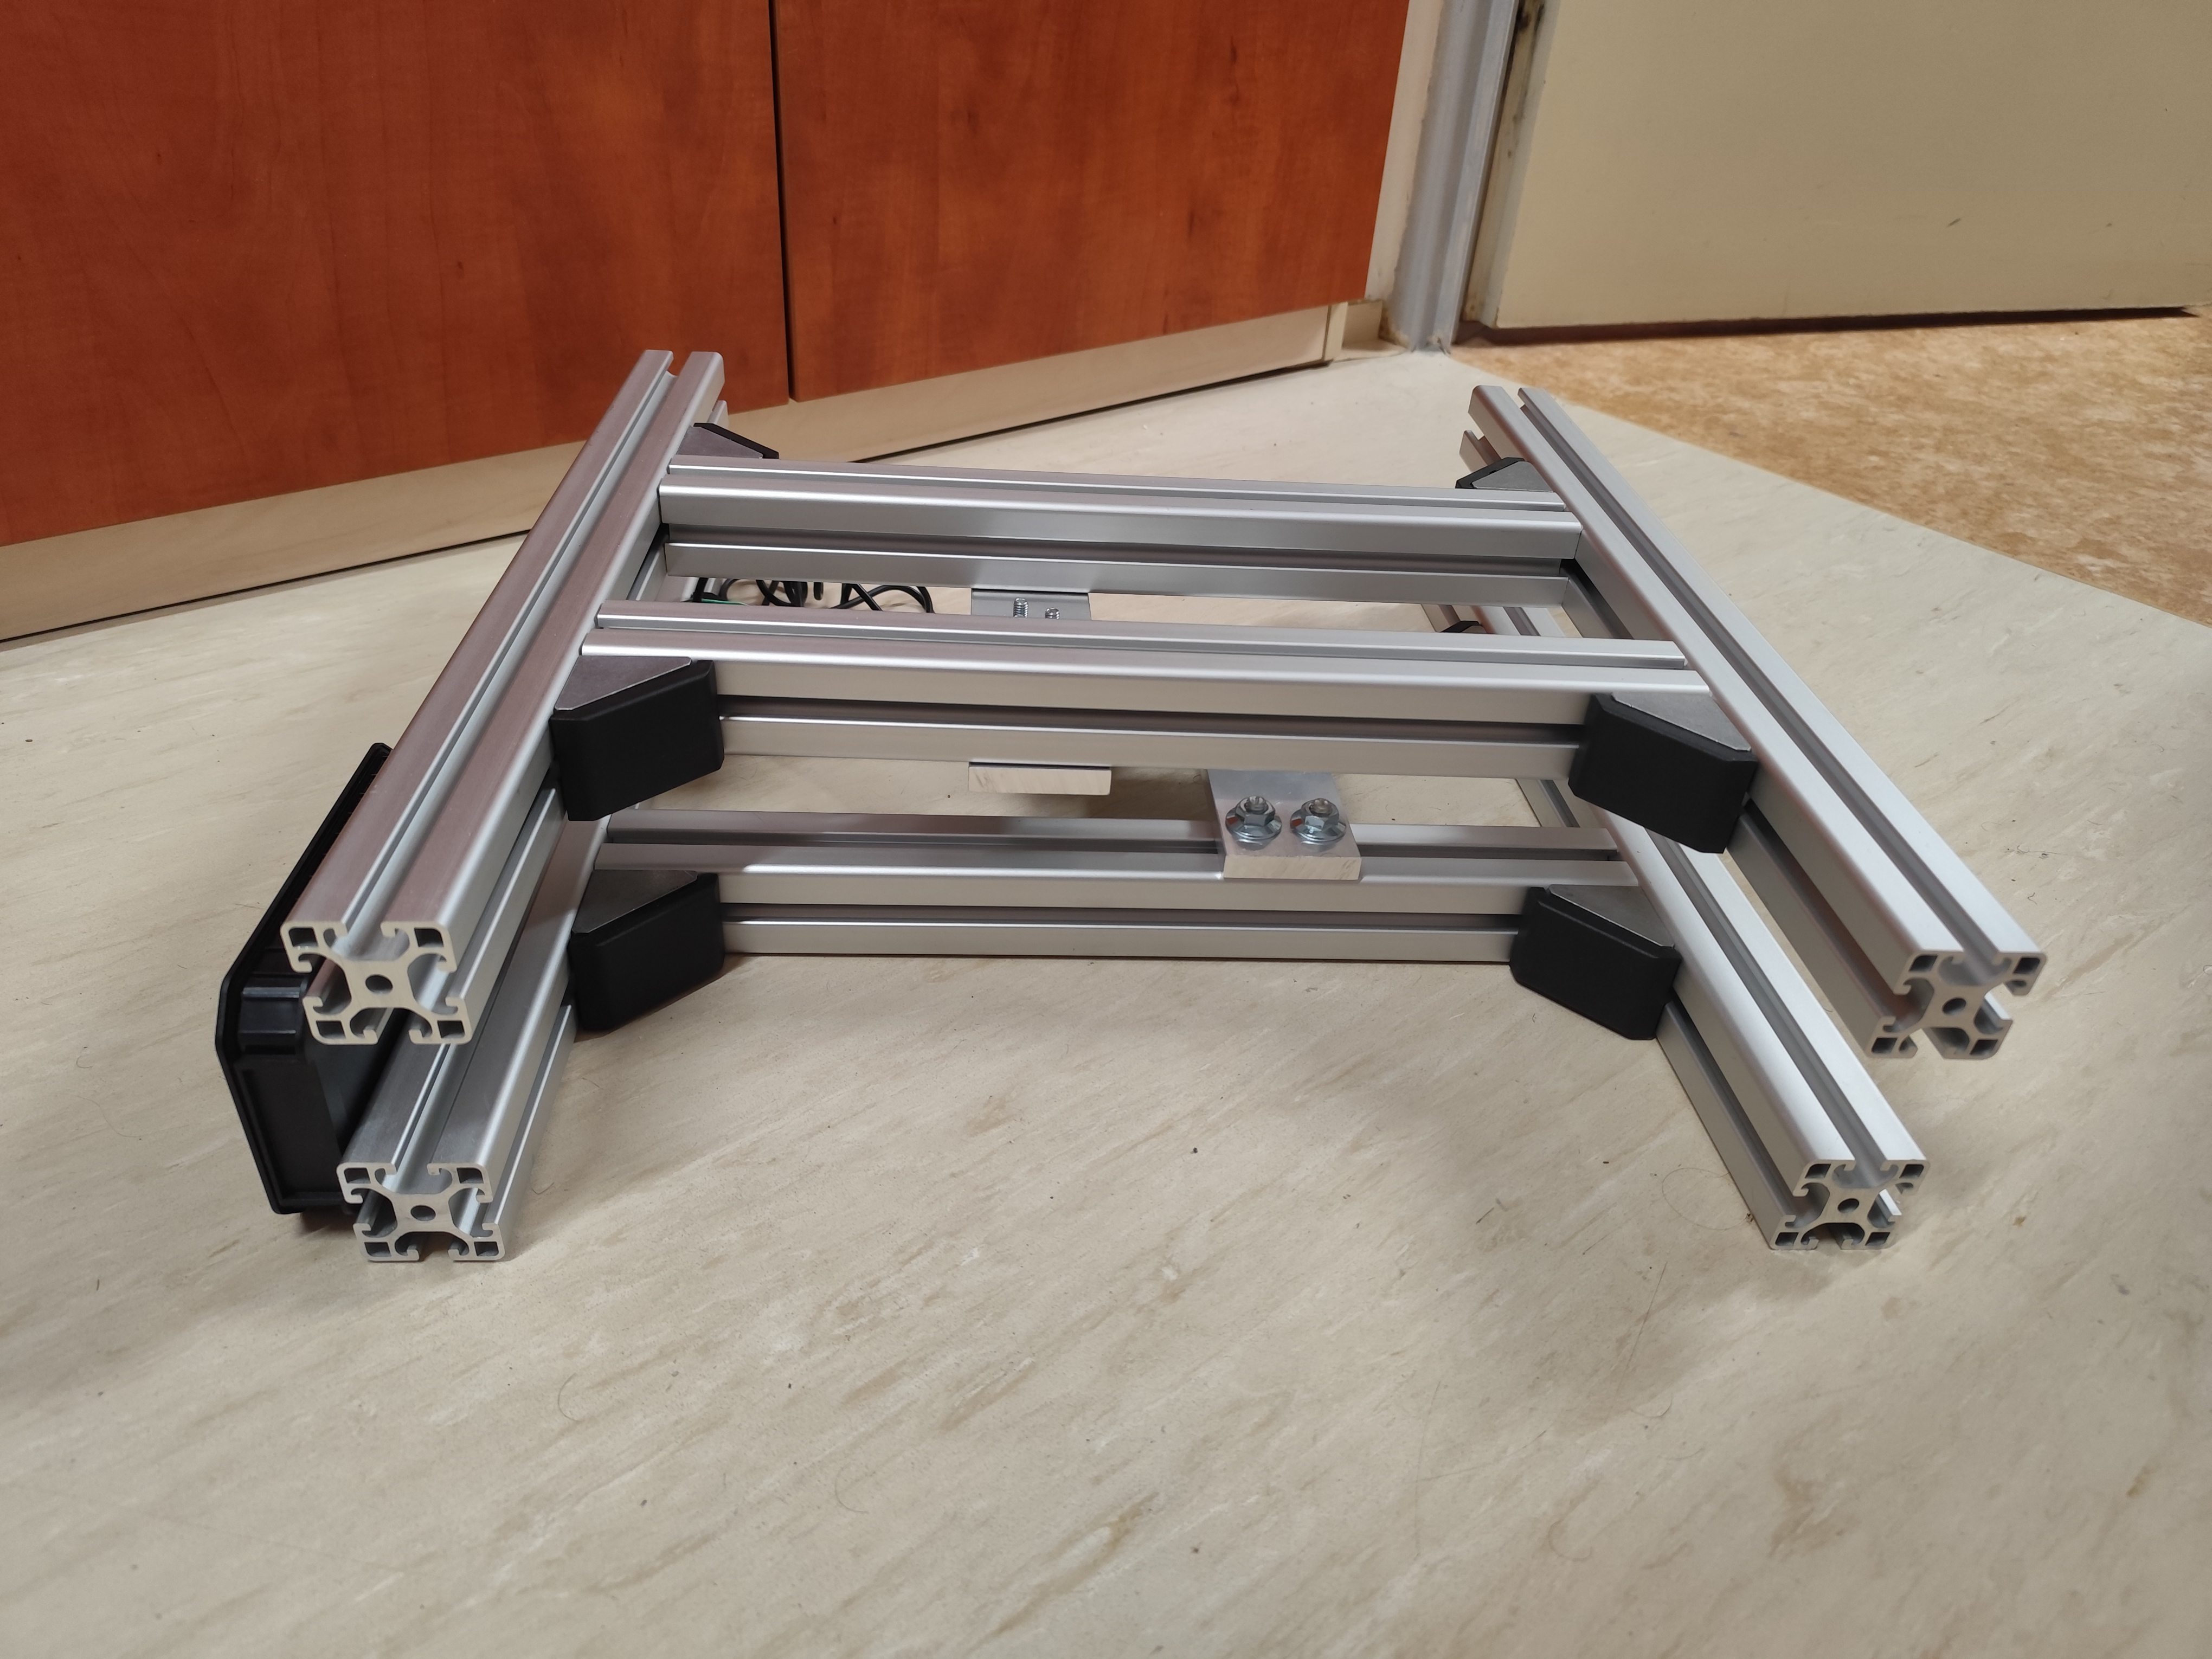
\includegraphics[width=0.7\textwidth]{obrazky-figures/konstrukce_ulove_vahy.jpg}
    \caption{Výsledná sestavená konstrukce úlové váhy.}
    \label{fig:konstrukce_ulove_vahy}
\end{figure}

Konstrukce úlové váhy byla realizována z~hliníkových profilů a spojovacích prvků určených pro modulární konstrukční systémy, jak bylo navrženo v~předchozí kapitole. Základ tvoří rám složený z~osmi profilů průřezu 40 $\times$ 40 mm (typ I8) -- čtyř o délce 460 mm a čtyř o délce 380 mm -- spojených hliníkovými úhelníky. Šrouby s~T-hlavou a přírubové matice určené pro~profilové drážky umožňují přesné polohování prvků a opakované rozebírání bez~poškození materiálu. Váhový senzor YZC-1B je uchycen mezi dvěma hliníkovými plochými tyčemi s~vyvrtanými otvory, které zajišťují rovnoměrný přenos zatížení na měřicí prvek. Výsledná konstrukce je zobrazena na obrázku \ref{fig:konstrukce_ulove_vahy} a přehled použitých komponent včetně cen uvádí tabulka \ref{tab:konstrukce_vaha}. Celková hmotnost rámu se pohybuje přibližně mezi 3 a 4~kg, což představuje vhodný kompromis mezi mechanickou stabilitou a snadnou manipulací při instalaci v~terénu.

\begin{table}[H]
    \centering
    \begin{tabular}{|c|c|c|}
    \hline
        \textbf{Položka} & \textbf{Počet kusů} & \textbf{Cena celkem} \\
        \hline
        Hliníkový profil lehký 40$\times$40 I8, 460 mm & 4 & 1209,76 Kč\\
        \hline
        Hliníkový profil lehký 40$\times$40 I8, 380 mm & 4 & 1034,94 Kč\\
        \hline
        Alu spojovací úhelník 40 & 8 & 484,97 Kč\\
        \hline
        Alu spojovací úhelník 40 -- kryt & 8 & 183,92 Kč\\
        \hline
        Přírubová matice & 24 & 124,87 Kč\\
        \hline
        Šroub s~T hlavou -- drážka I8 & 24 & 394,94 Kč\\
        \hline
        Hliníková tyč plochá 50$\times$10, 180 mm & 2 & 138 Kč\\
        \hline
        Matice s~límcem M6 & 6 & 5,8 Kč\\
        \hline
        Šrouby M6 & 6 & 13,5 Kč\\
        \hline
        Pérové podložky & 6 & 7,5 Kč\\
        \hline
        \multicolumn{2}{|c|}{\textbf{Cena celkem}} & \textbf{3598,2 Kč} \\
        \hline
    \end{tabular}
    \caption{Přehled použitých komponent pro konstrukci úlové váhy.}
    \label{tab:konstrukce_vaha}
\end{table}

Řídicí jednotkou senzorového modulu je mikrokontrolér ESP32-S3 (LilyGO TTGO T-Display-S3) uložený spolu s~ostatní elektronikou v~krabičce s~krytím IP66. Kabeláž je vyvedena přes průchodky zajišťující těsnost i po doplnění dalšího otvoru pro přidaný senzor. Převodník HX711 zpracovává analogový signál tenzometru a komunikuje s~mikrokontrolérem přes dvoudrátové rozhraní. Venkovní teplota je měřena senzorem DS18B20 připojeným přes sběrnici 1-wire s~pull-up rezistorem 6,8 k$\Omega$ -- standardně doporučovanou hodnotu 4,7~$k\Omega$ jsem neměla k~dispozici, avšak při délce kabelu 1 m vyšší odpor komunikaci neovlivňuje. Senzor BME280 měřící vnitřní teplotu, vlhkost a tlak je připojen přes sběrnici I\textsuperscript{2}C a umístěn v~ochranném obalu v~horní části úlu (viz obrázek \ref{fig:umisteni_vnitrniho_senzoru}).

\begin{figure}[H]
    \centering
    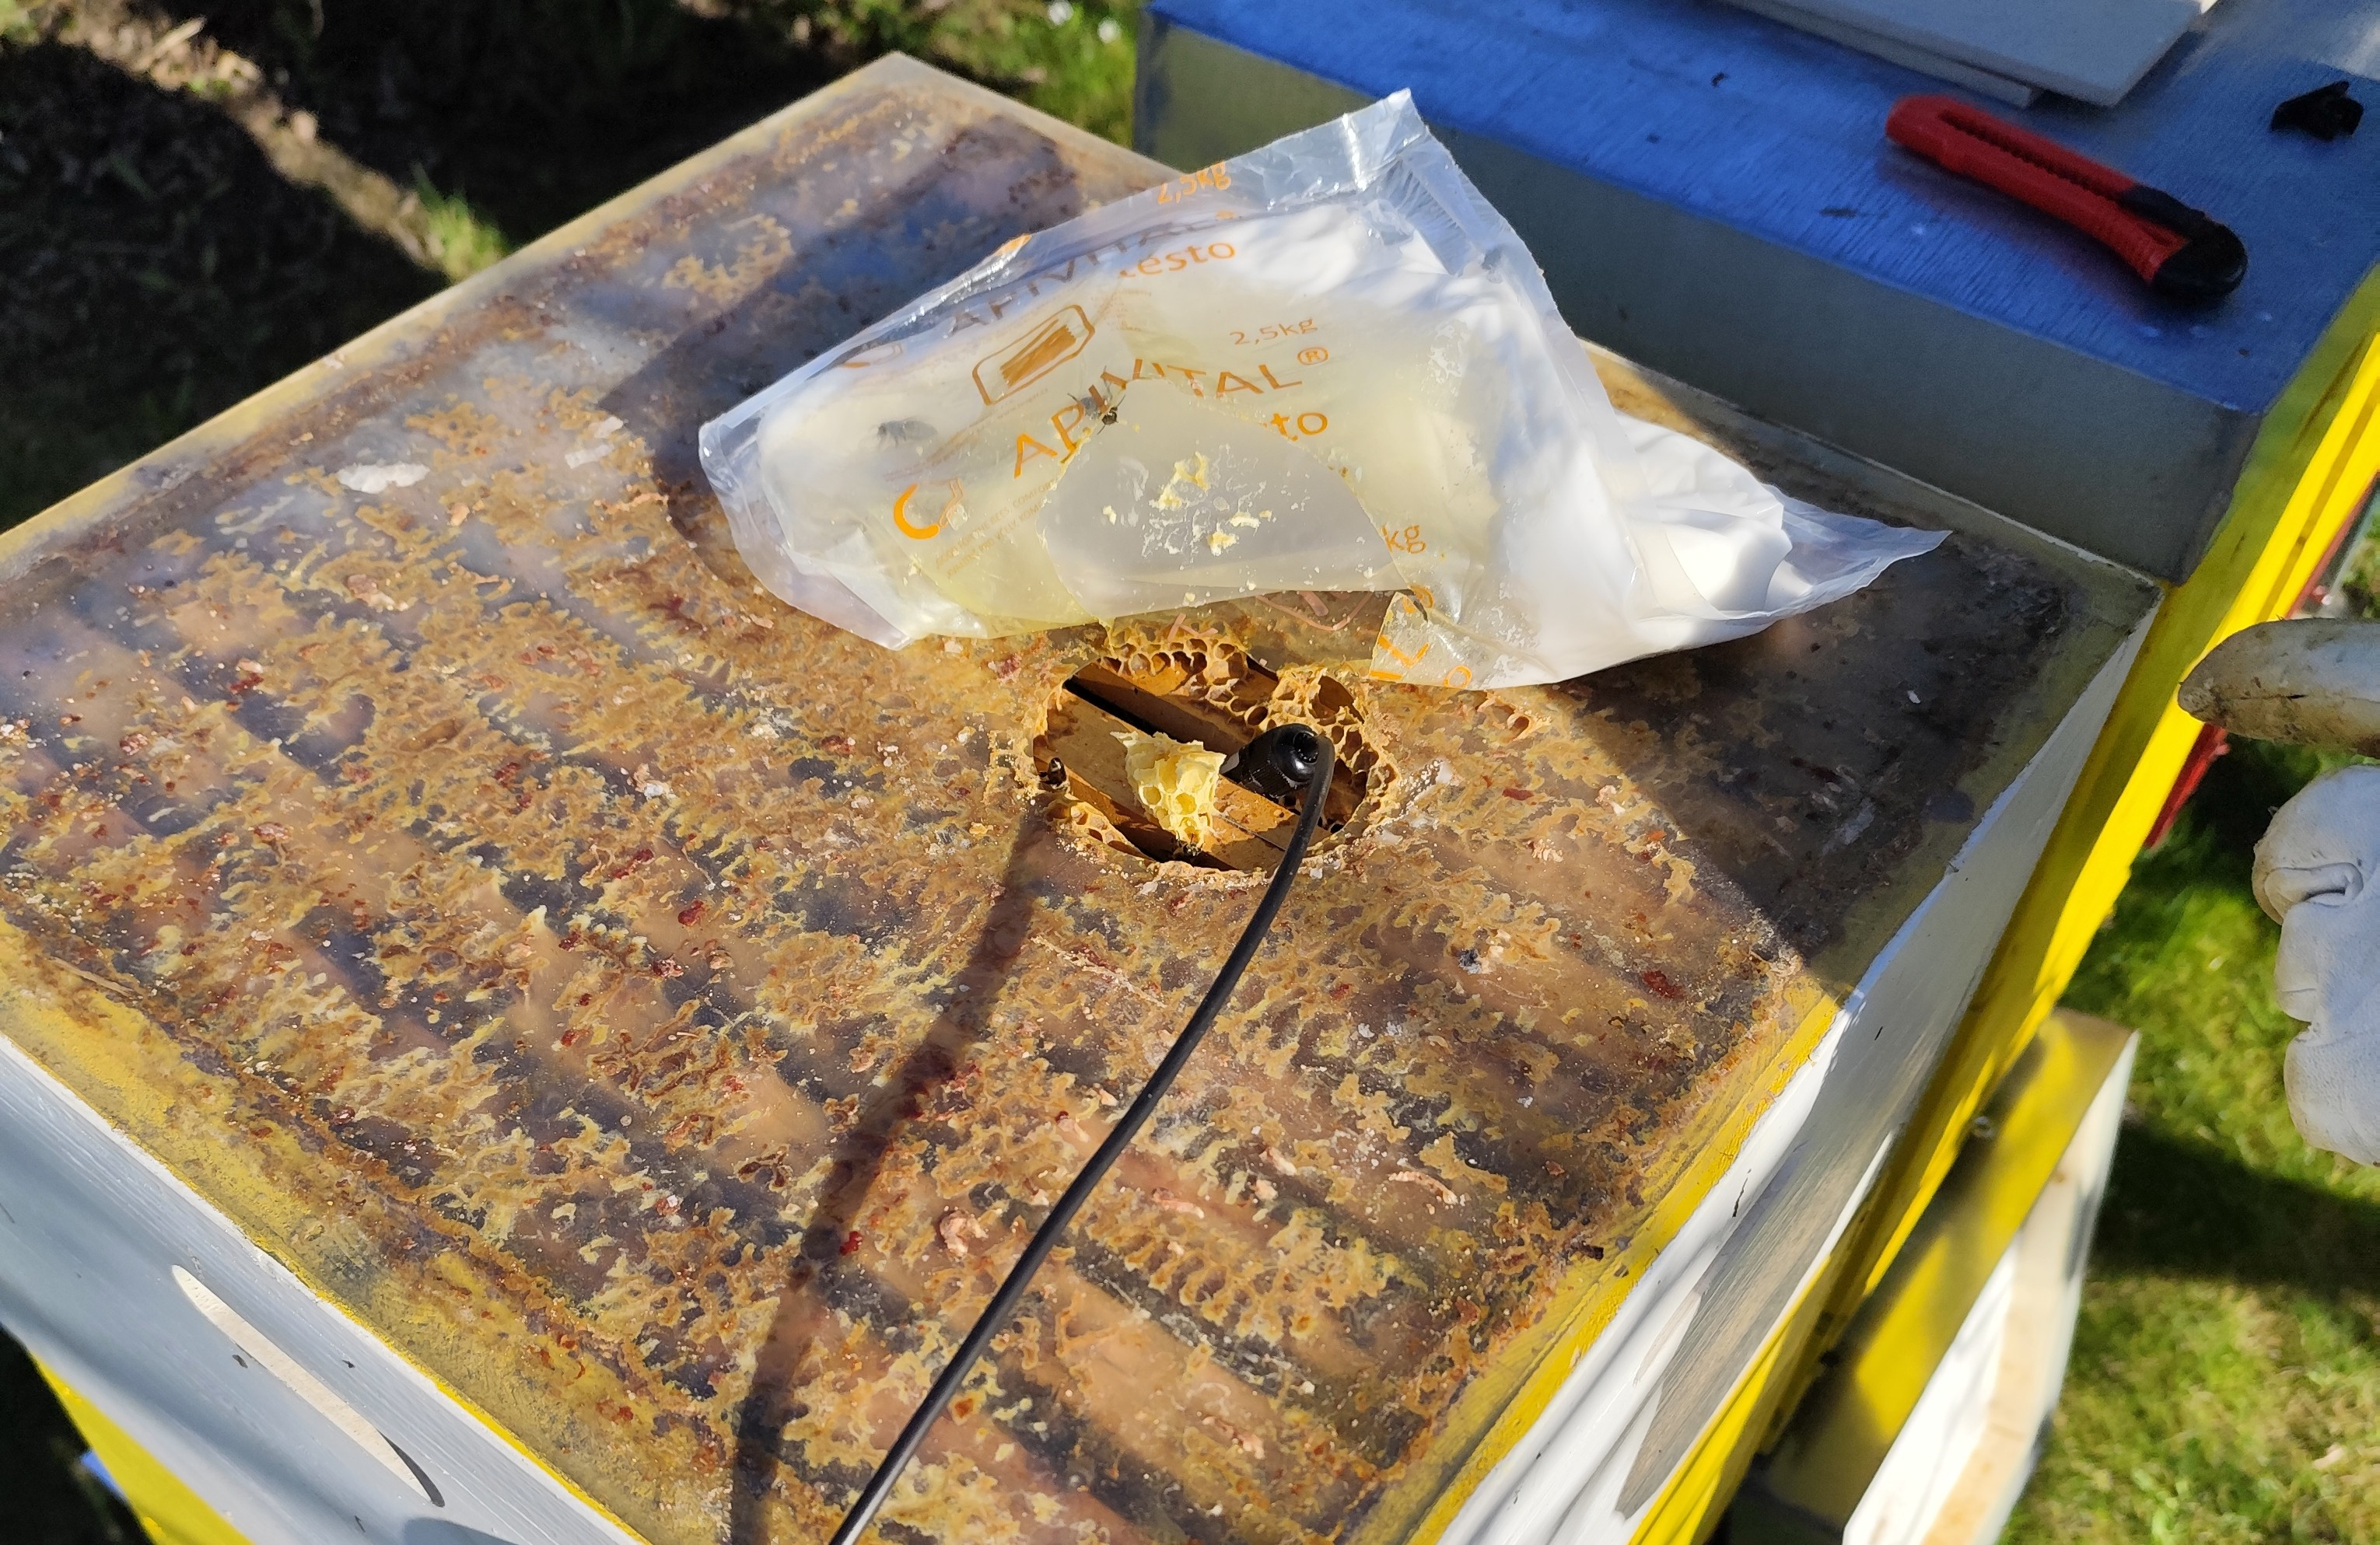
\includegraphics[width=0.7\textwidth]{obrazky-figures/umisteni_vnitrniho_senzoru.jpg}
    \caption{Pozice umístění senzoru BME280 uvnitř úlu.}
    \label{fig:umisteni_vnitrniho_senzoru}
\end{figure}

V~první verzi zařízení byl pro měření venkovní teploty použit senzor DHT11. Po instalaci začátkem března však docházelo k~jeho opakovanému provozu mimo specifikovaný teplotní rozsah 0 až +50\,°C, což vedlo k~poruše mikrokontroléru projevující se neschopností navázat Wi-Fi připojení a výrazným zahříváním. Senzor byl proto nahrazen vodotěsnou verzí DS18B20 s~rozsahem $-55$ až $+125$\,°C plně postačujícím pro celoroční venkovní provoz.

\subsection*{Konstrukce kamerového modulu}
Kamerový modul byl vyroben technologií 3D tisku na tiskárně Bambu Lab A1 Mini s~tiskovým objemem 180 $\times$ 180 $\times$ 180 mm.  Omezený tiskový prostor si vyžádal rozdělení konstrukce do více samostatných částí, což však zároveň usnadňuje manipulaci a případné budoucí úpravy. Jako materiál jsem zvolila bílý filament PLA (Elegoo, 1 kg), který je snadno tisknutelný, cenově dostupný a dostatečně pevný. Bílá barva navíc snižuje absorpci slunečního záření a poskytuje vhodný kontrast vůči zbarvení včel. Celková spotřeba filamentu činí 682,07 g při době tisku 1~den 13~hod 12~min, s výplní 15\,\% a rozměry sestavy 174~$\times$~174~$\times$~221~mm. Spotřebu materiálu na jednotlivé díly uvádí tabulka \ref{tab:spotreba_filamentu}.

\begin{table}[H]
    \centering
    \begin{tabular}{|l|c|c|}
    \hline
        \textbf{Část} & \textbf{Spotřeba filamentu [g]} & \textbf{Čas tisku} \\
        \hline
        Střecha & 55,42 & 1 hod 34 min \\
        \hline
        Vrchní část & 173,70 & 10 hod 48 min \\
        \hline
        Obvodové stěny & 250,27 & 13 hod 40 min \\
        \hline
        Difúzní vrstva & 9,67 & 22 min 39 s \\
        \hline
        Tunelové průchody & 54,37 & 2 hod 14 min \\
        \hline
        Spodní část (40 $\times$ 164 mm) & 138,63 & 8 hod 11 min \\
        \hline
        \textbf{Celkem} & \textbf{682,07} & \textbf{37 hod 12 min} \\
        \hline
    \end{tabular}
    \caption{Spotřeba filamentu PLA a čas tisku jednotlivých částí kamerového modulu.}
    \label{tab:spotreba_filamentu}
\end{table}

Oproti předchozí práci \cite{Chovancova2025}, kde byly obvodové stěny realizovány z~odlišného materiálu, tvoří v~tomto návrhu celý plášť modulu jeden tištěný celek, čímž se zjednodušuje výroba i instalace. Spodní část modulu slouží jako rozšíření letáku přesně odpovídající výšce česna -- není proto nutné žádné dodatečné uchycení. Součástí je průhledná deska z~plexiskla, která brání včelám ve vstupu do zařízení a zároveň udržuje definovanou vzdálenost 16,5~cm mezi včelami a kamerou. Vyjímatelný modul s~tunelovými průchody usměrňuje pohyb včel a snižuje jejich vzájemné překryvy při snímání. Horní část nese kameru a Raspberry Pi 5 a je uzavřena krytem chránícím elektroniku před povětrnostními vlivy a kontaktem se včelami.

V~průběhu realizace jsem musela řešit dva problémy. Původně použitý klasický LED pásek rozdělený na segmenty a propojený pájením se ukázal jako mechanicky nespolehlivý. Byl proto nahrazen flexibilním LED neonovým páskem TR-34N napájeným přes USB, který nevyžaduje pájení a je odolnější vůči mechanickému namáhání (viz obrázek \ref{fig:osvetleni_kameroveho_modulu}). Druhým problémem byly nežádoucí odrazy světla na plexisklu. Tento jev byl odstraněn doplněním tenké difuzní vrstvy vytištěné z~pouhých dvou tiskových vrstev PLA, která zajišťuje rovnoměrný rozptyl světla při zachování dostatečné propustnosti.

\begin{figure}[H]
    \centering
    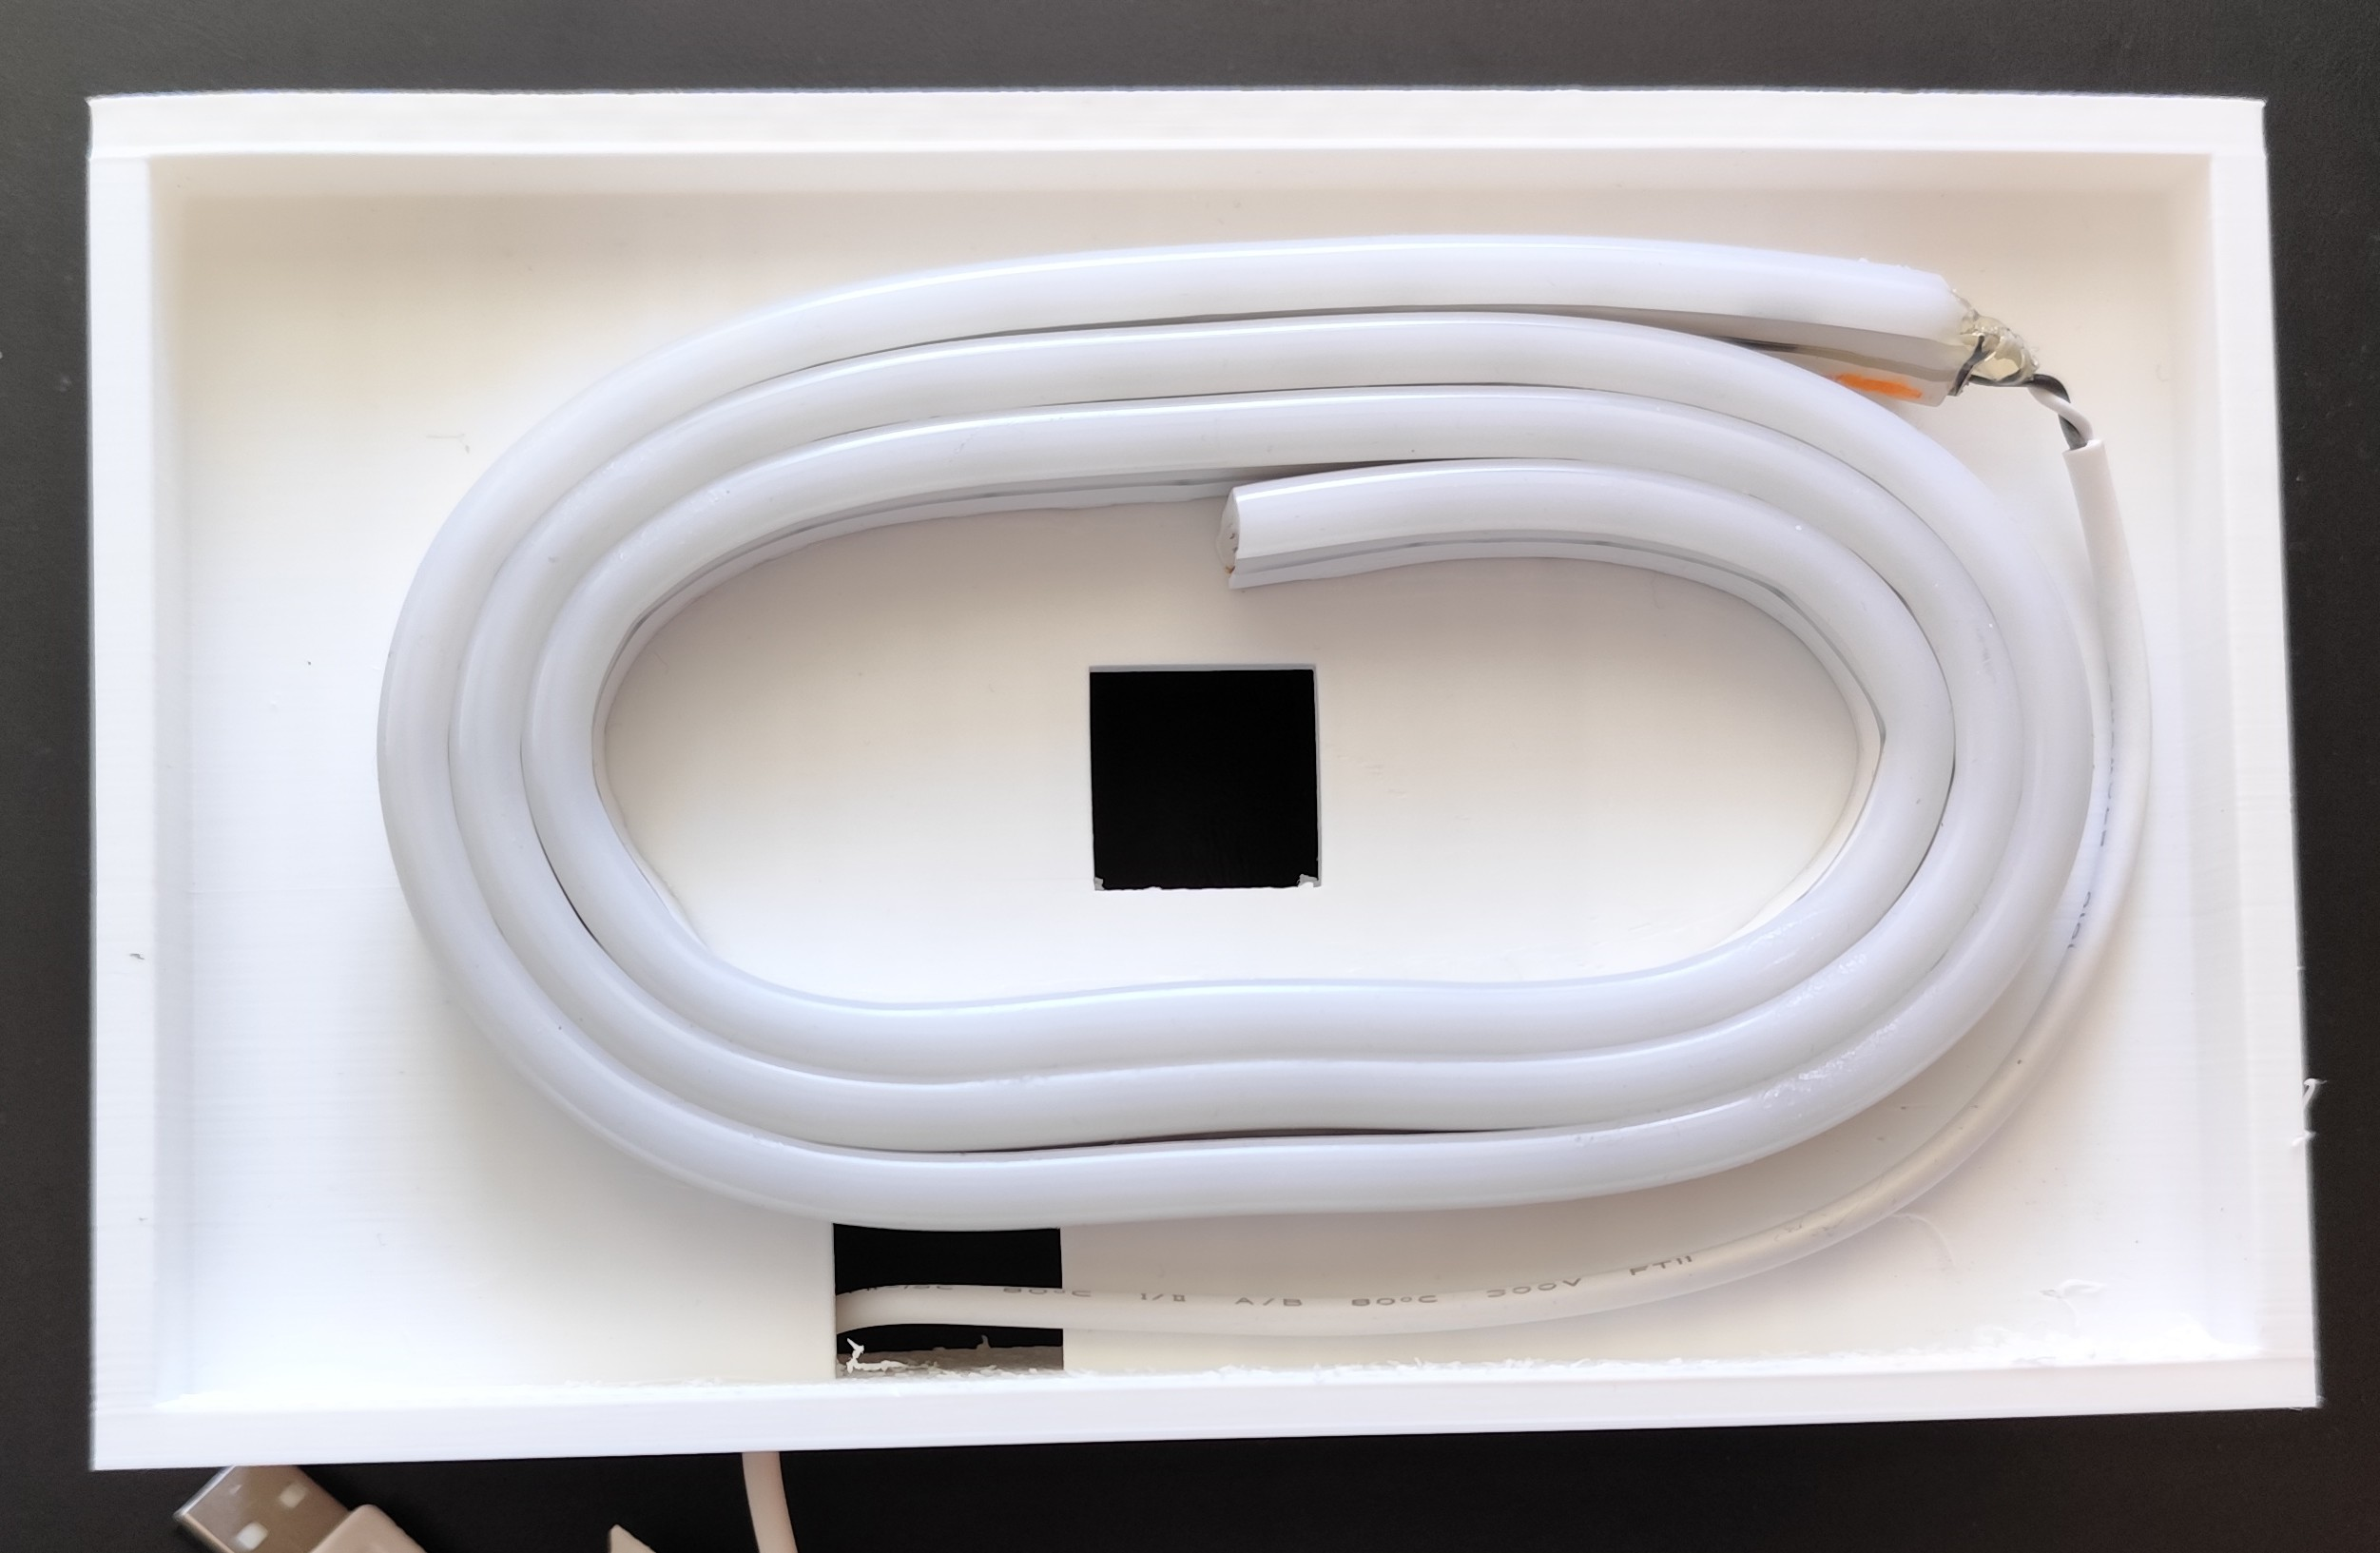
\includegraphics[width=0.5\textwidth]{obrazky-figures/osvetleni_kameroveho_modulu.jpg}
    \caption{Umístění LED pásku v horní části.}
    \label{fig:osvetleni_kameroveho_modulu}
\end{figure}

\subsection*{Napájení} 
Napájecí soustava převzatá z~předchozí práce \cite{Chovancova2025} kombinuje solární panel, AGM akumulátor a PWM regulátor nabíjení. Senzorový modul je napájen prostřednictvím USB výstupu regulátoru. Kamerový modul s~Raspberry Pi 5 je vzhledem ke své výrazně vyšší energetické náročnosti napájen samostatně ze síťového zdroje -- toto rozhodnutí je podrobněji zdůvodněno v~kapitole věnované testování, sekce \ref{sec:napajeni_systemu}.

\subsection*{Konečná podoba systému} 

\begin{figure}[H]
    \centering
    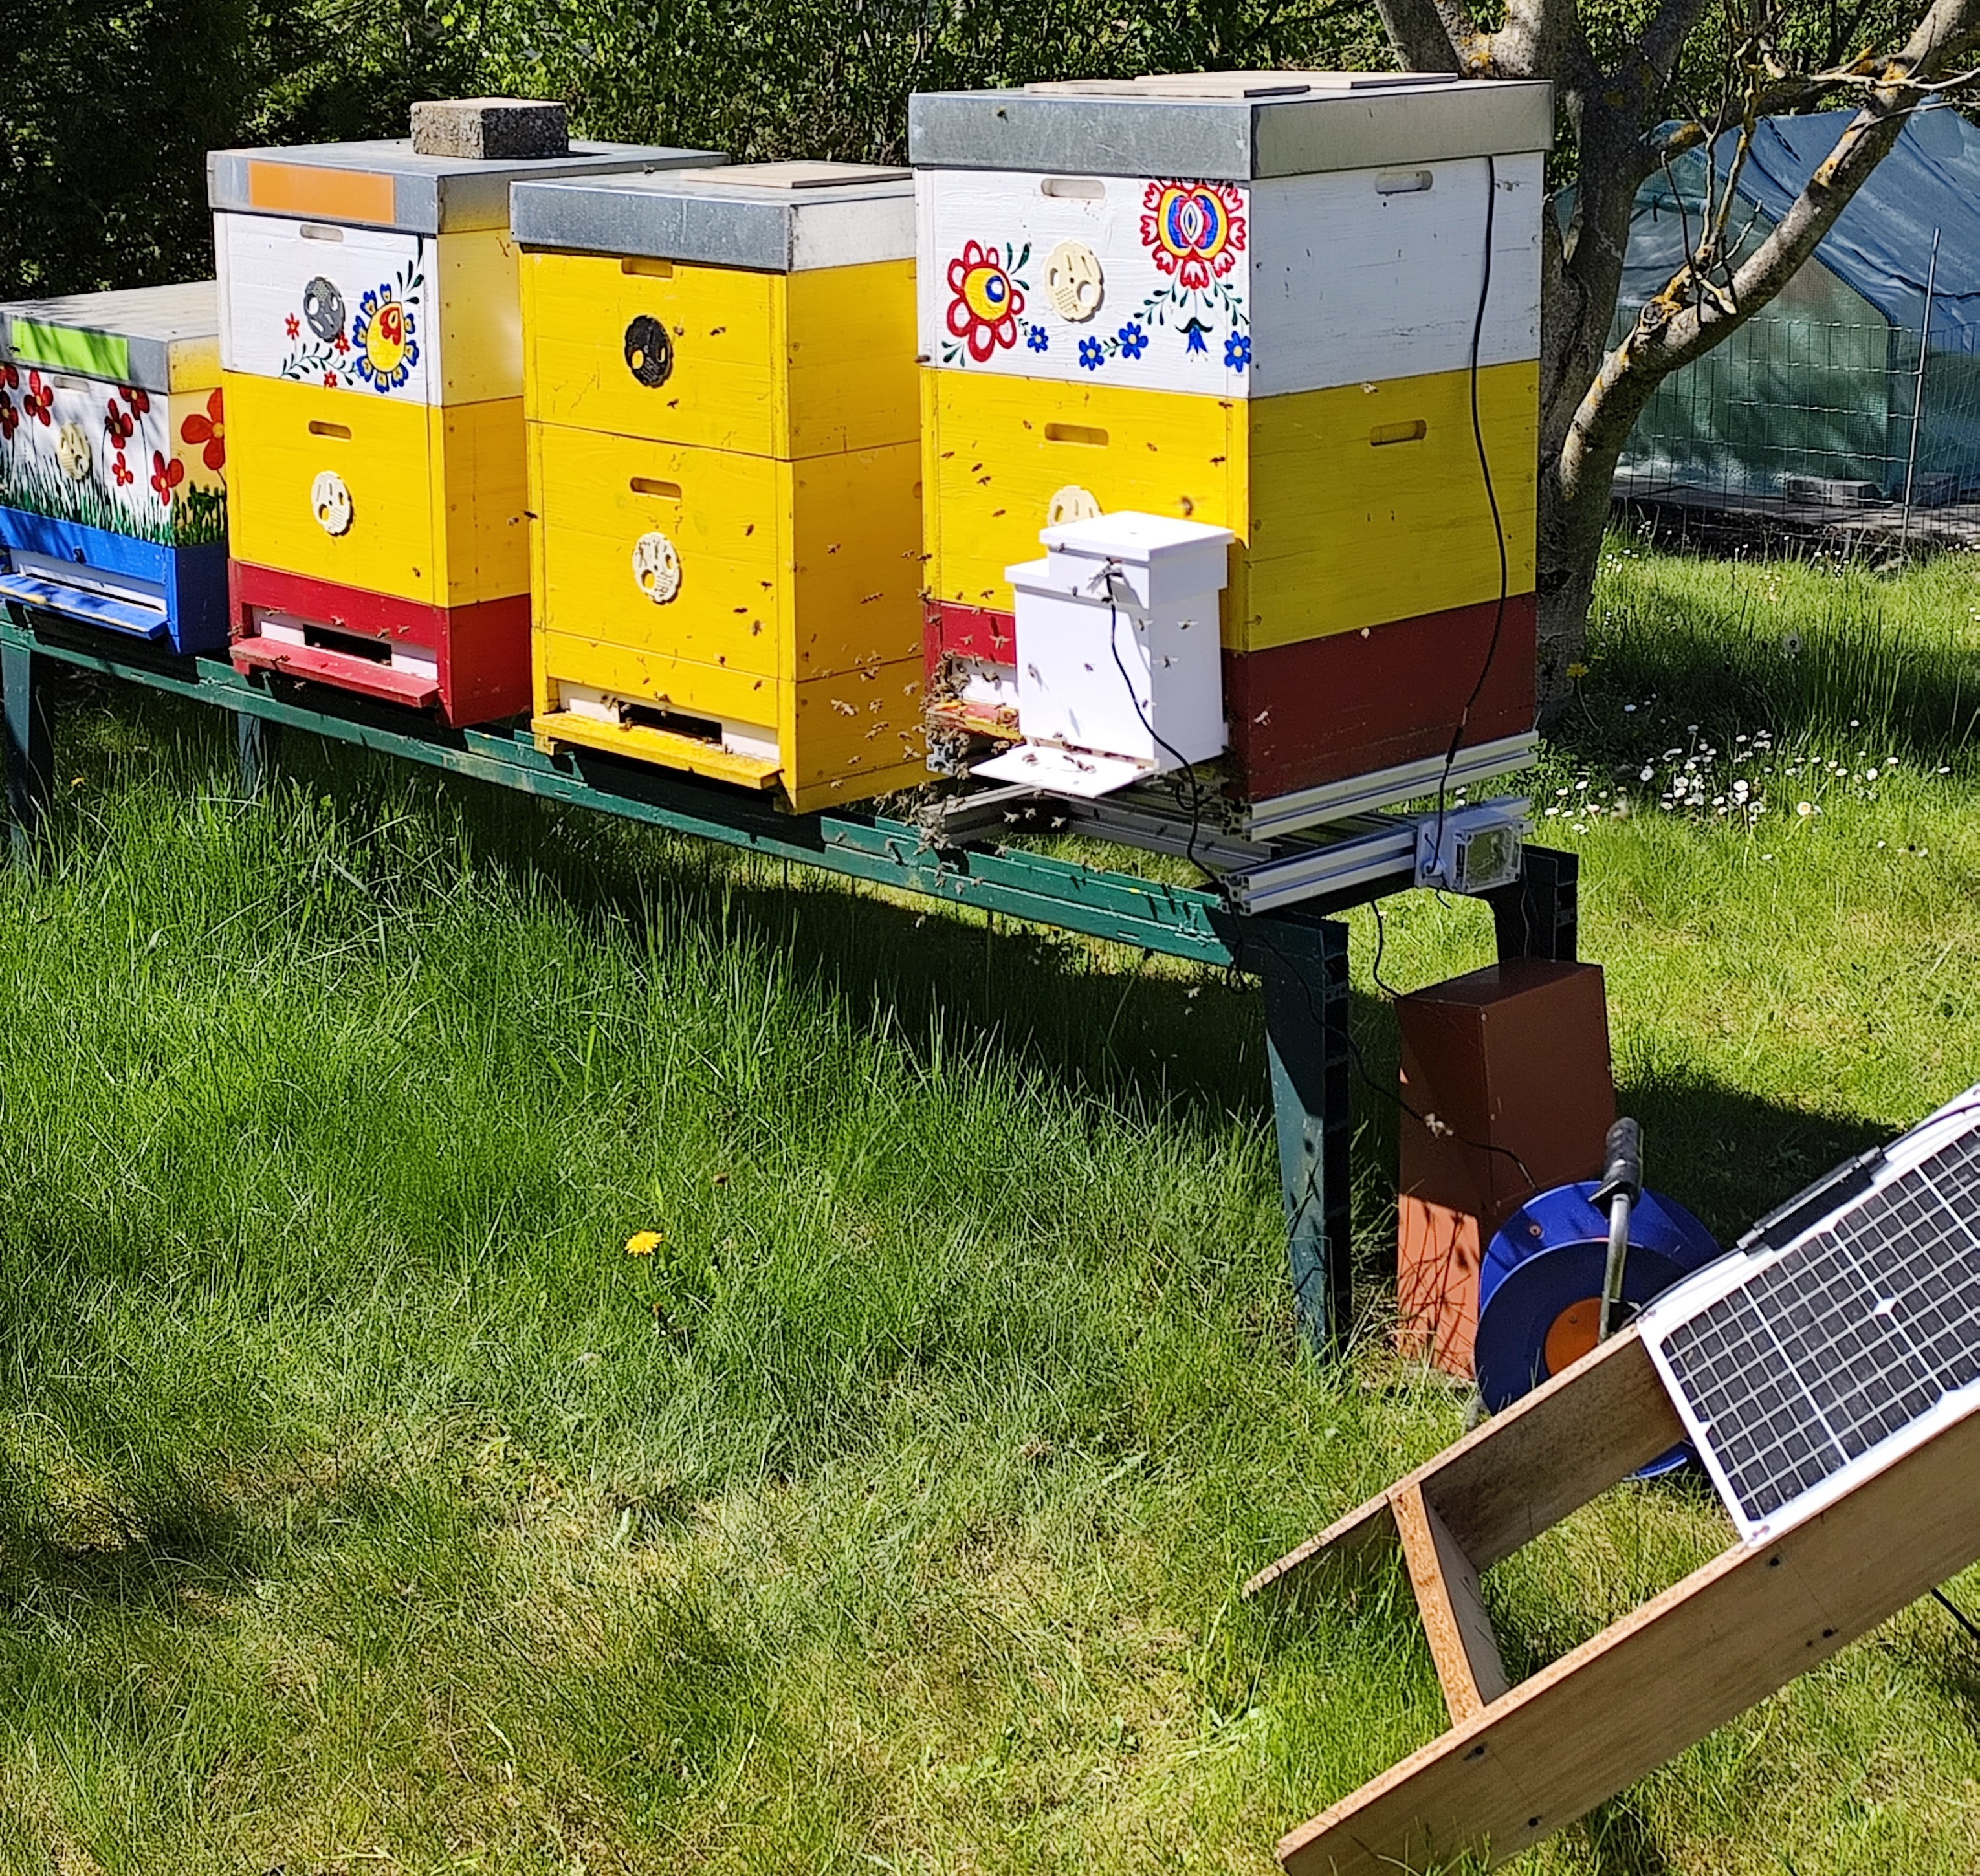
\includegraphics[width=\textwidth]{obrazky-figures/finalni_podoba.jpg}
    \caption{Finální podoba zařízení.}
    \label{fig:finalni_podoba}
\end{figure}

\begin{table}[H]
    \centering
    \begin{tabular}{|l|c|}
    \hline
        \textbf{Název položky} & \textbf{Cena} \\
        \hline
        Elegoo PLA 1kg White & 319 Kč \\
        \hline
        Gutta Plexisklo Hobbyglass transparentní, 250 $\times$ 500 $\times$ 2 mm & 84,87 Kč \\
        \hline
        Konstrukce úlové váhy & 3\,598,20 Kč \\
        \hline
        Hardwarové komponenty & 9\,192,51 Kč \\
        \hline
        \textbf{Celková cena zařízení} & \textbf{13\,194,58 Kč} \\
        \hline
    \end{tabular}
    \caption{Celková cena použitých materiálů a hardwarových komponent.}
    \label{tab:celkova_cena_zarizeni}
\end{table}

\section{Datové sady}
Tato sekce popisuje veškerá data využitá při vývoji systému -- jak veřejně dostupné datové sady, tak data nasbíraná vlastním zařízením. Přehled použitých existujících datových sad je uveden v~tabulce~\ref{tab:vyuzite_datasety}.

\begin{table}[H]
    \centering
    \begin{tabular}{|m{4.5cm}|m{8cm}|}
    \hline
        \textbf{Třídy} & \textbf{Zdroj} \\
        \hline
        časové řady (hmotnost, teplota, vlhkost, tlak) & \cite{BeeObserver} \\
        \hline
        včela, vosa, sršeň & \url{https://universe.roboflow.com/hornets/hornet-asu50} \\
        \hline
        vosa & \url{https://universe.roboflow.com/dectection-r62lz/wasp-detection-hudm3} \\
        \hline
        trubec, včela, pylová včela, matka & \url{https://universe.roboflow.com/workspace-1-tu7e5/bee-detection-h59jf} \\
        \hline
        včela bez pylu, pylová včela & \url{https://universe.roboflow.com/first-yeaie/honeybee-pollen-detect} \\
        \hline
        sršeň & \url{https://universe.roboflow.com/autobee/vespa-velutina} \\
        \hline
        sršeň & \url{https://universe.roboflow.com/autobee/vespa-2} \\
        \hline
        včela, pylová včela & \url{https://universe.roboflow.com/labelbee/bee_pollen-2024_04-v2-1} \\
        \hline
    \end{tabular}
    \caption{Přehled použitých datových sad.}
    \label{tab:vyuzite_datasety}
\end{table}

\subsection*{Veřejně dostupné datové sady}

\subsubsection*{BeeObserver (BoB)}
Primární datová sada pro vývoj modelů časových řad pochází z~projektu BeeObserver \cite{BeeObserver}, který v~letech 2019--2022 kontinuálně monitoroval včelstva umístěná na stanovištích v~Německu. Dataset obsahuje agregovaná senzorová data (v~denních, hodinových a minutových intervalech) ze 78 kolonií napříč čtyřmi roky, přičemž ne všechny kolonie mají k~dispozici záznamy pro celé sledované období. Pro účely navrhovaného řešení jsem využila hodinovou variantu dat (\texttt{\_h}) zahrnující veličiny odpovídající senzorickému vybavení navrženého systému: hmotnost úlu (\texttt{weight\_kg\_noOutlier}), změnu hmotnosti (\texttt{weight\_delta\_noOutlier}), venkovní teplotu (\texttt{t\_o}), relativní vlhkost (\texttt{h}), vnitřní teplotu středového rámku (\texttt{t\_i\_3}), vnitřní teplotu (\texttt{t}) a atmosférický tlak (\texttt{p}). Dataset byl zvolen jako vývojová základna zejména proto, že jeho senzorická sestava přesně odpovídá měřeným veličinám nasazeného senzorového modulu, a lze jej tedy přímo využít jako náhradu vlastních dat při vývoji a ladění modelů.

\subsubsection*{Datové sady pro počítačové vidění}
Pro trénování modelů počítačového vidění byla sestavena komplexní anotovaná datová sada sloučením několika veřejně dostupných datových sad pocházejících z~platformy Roboflow. Třídy jednotlivých zdrojových sad byly sjednoceny a upraveny do pěti výsledných tříd: standardní včela (\textit{bee}), včela nesoucí pyl (\textit{pollen bee}), včelí matka (\textit{queen}), vosa (\textit{wasp}) a sršeň (\textit{hornet}). 

Tato sloučená sada posloužila jako základ pro trénování prvního modelu a jako zdroj pro předběžnou anotaci vlastních snímků.

\subsection*{Vlastní datové sady}

\subsubsection*{Senzorová data}
Vlastní senzorová data byla nasbírána nasazeným systémem v~průběhu jednoho týdne z~jediného úlu. V pětiminutovém intervalu vzorkování bylo zaznamenáváno pět veličin: hmotnost úlu (\texttt{weight}), venkovní teplota (\texttt{t\_o}), vnitřní teplota (\texttt{t}), relativní vlhkost (\texttt{h}) a atmosférický tlak (\texttt{p}). Data neobsahují výpadky ani chybějící hodnoty. Ačkoliv týdenní délka záznamu neumožňuje zachytit sezónní dynamiku včelstva, slouží jako primární validační sada pro ověření funkčnosti nasazeného systému v~reálných podmínkách. Pro samotný vývoj a trénování modelů byla proto využita datová sada BeeObserver.

\subsubsection*{Obrazová data}
Vlastní obrazová data byla pořízena kamerovým modulem nasazeným na česnu úlu. Z~původního souboru přibližně 1300 snímků bylo po manuální kontrole kvality použitelných pouze 435. Hlavním důvodem vyřazení většiny snímků bylo vzájemné překrývání včel v~záběru (viz obrázek \ref{fig:vysoka_aktivita}) -- při vyšší letové aktivitě se jedinci překrývají takovým způsobem, že jejich individuální anotace není spolehlivě proveditelná, a takovéto snímky by do trénovací sady zanášely šum. Snímky byly nejdříve anotovány prvním natrénovaným modelem (YOLO26n) a následně manuálně zkontrolovány a opraveny, protože kvalita automatické anotace nebyla dostatečná pro přímé použití. Vzhledem k~dostupnosti vlastních dat pouze pro dvě třídy (\textit{bee} a \textit{pollen bee}) jsem všechny ostatní třídy vyřadila.

\begin{figure}[H]
    \centering
    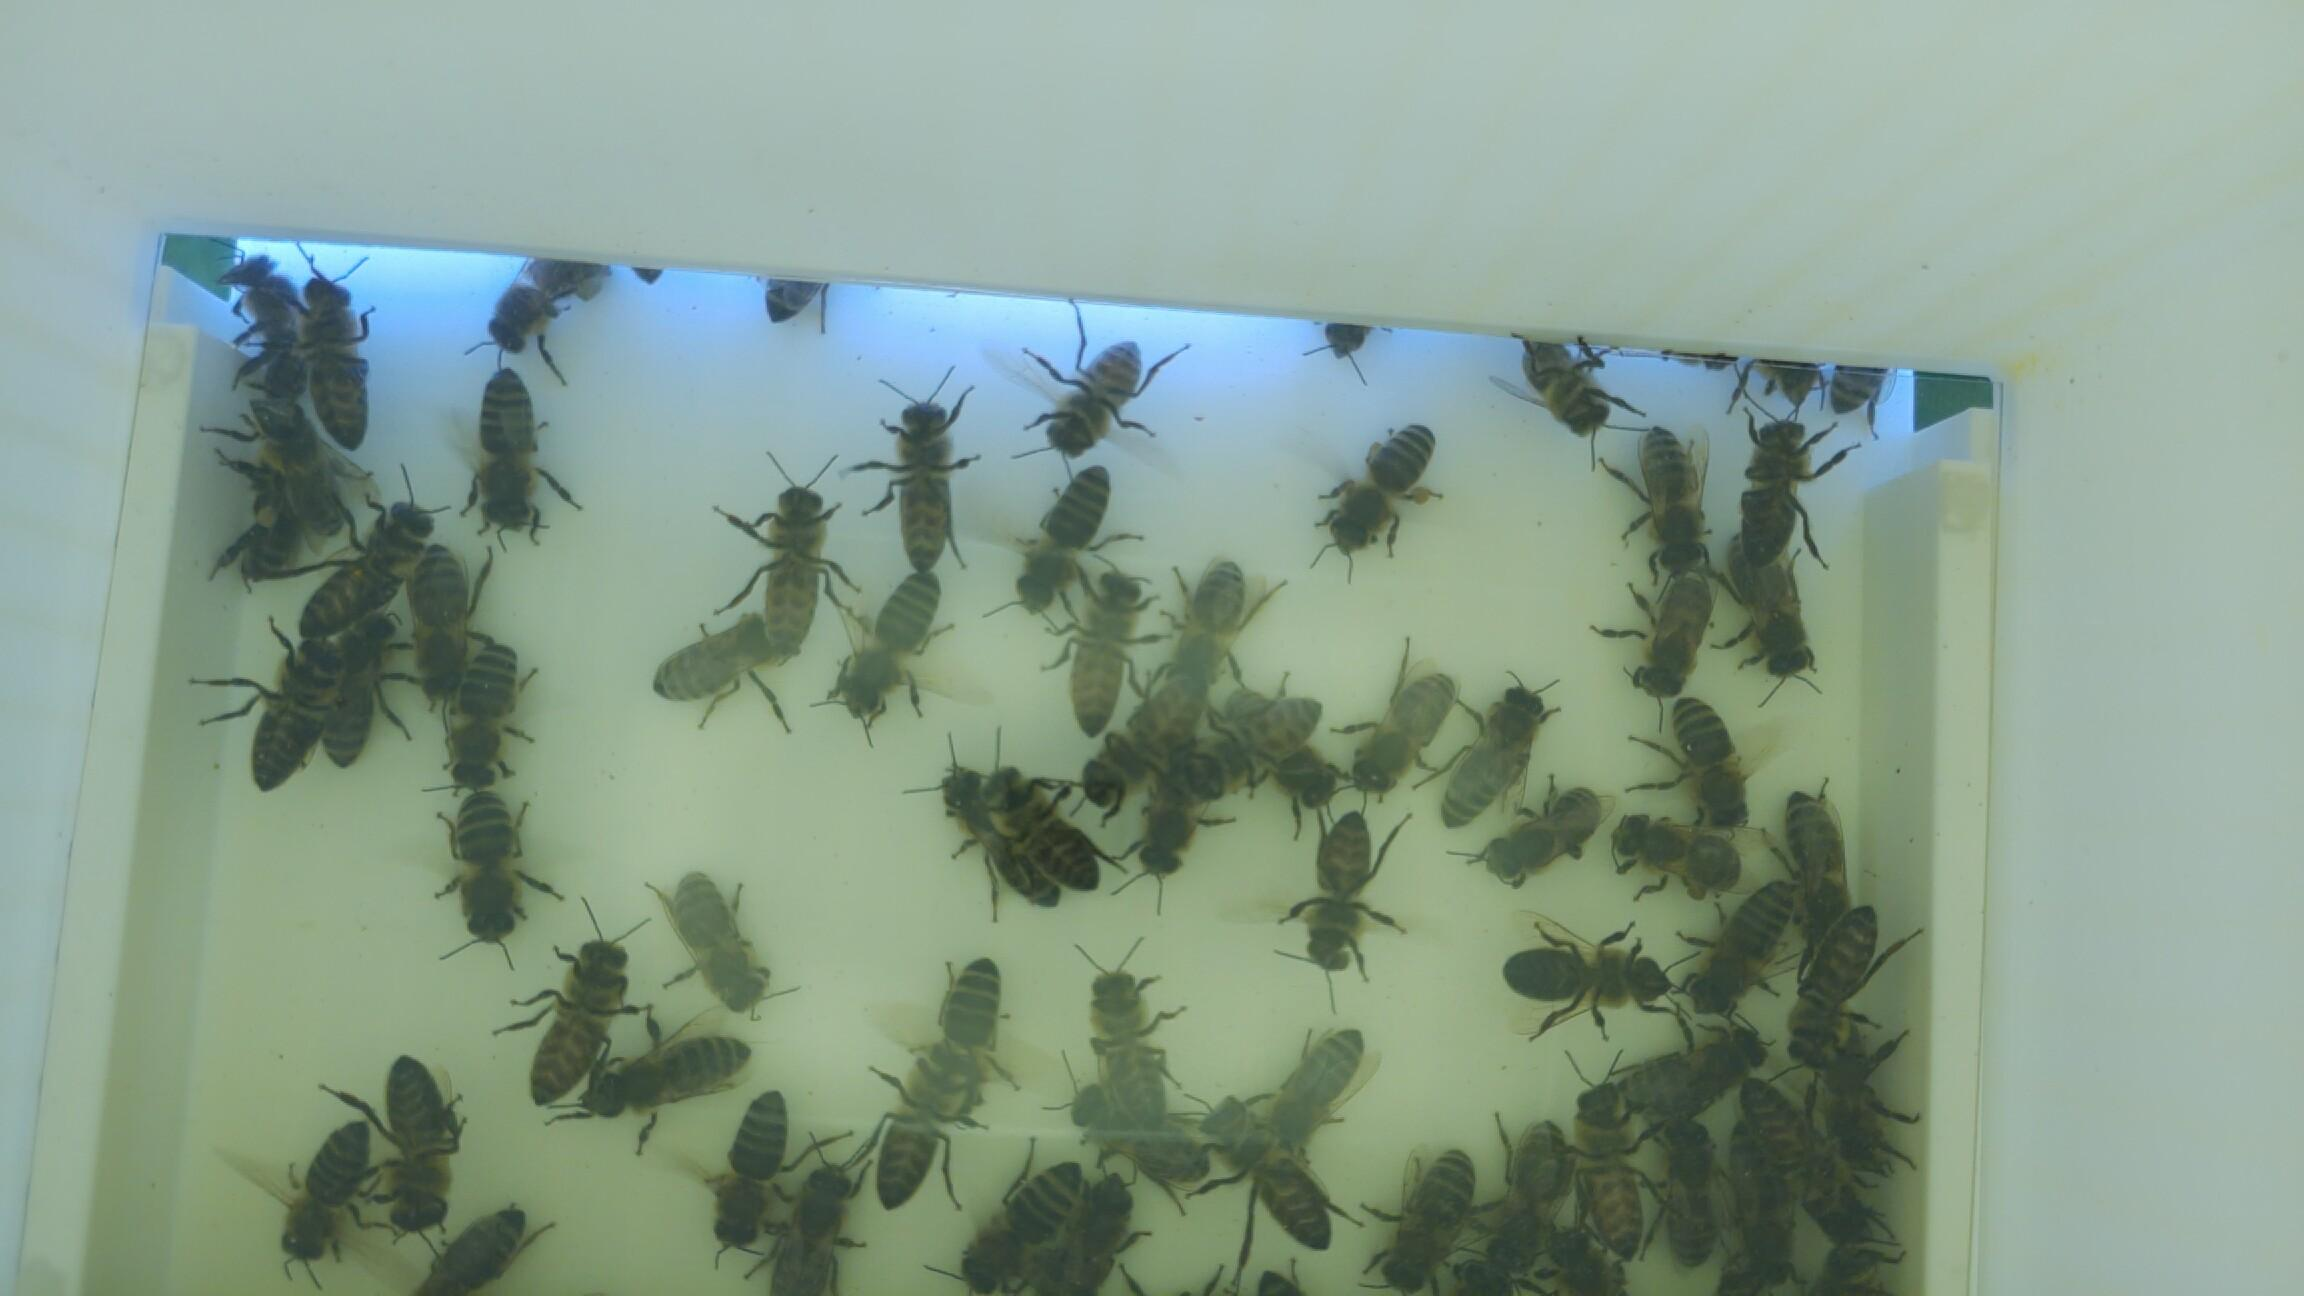
\includegraphics[width=0.5\textwidth]{obrazky-figures/vysoka_aktivita.jpg}
    \caption{Snímek ukazující vysokou aktivitu včel.}
    \label{fig:vysoka_aktivita}
\end{figure}

Na základě vlastních snímků jsem sestavila dvě trénovací sady:
\begin{itemize}
    \item \textbf{my\_bee\_detection}\,\footnotemark[2] -- pouze vlastní anotované snímky (435 snímků, třídy \textit{bee} a \textit{pollen bee})
    \item \textbf{bee\_detection\_merged}\,\footnotemark[2] -- veřejná komplexní sada rozšířená o~vlastní snímky (4566 snímků, všech pět tříd)
\end{itemize}

\footnotetext[2]{Datové sady jsou dostupné zde: \url{https://app.roboflow.com/beekeeper5-1lsdm}}

\subsection*{Předzpracování dat}

\subsubsection*{Časové řady}
Dataset BeeObserver byl pro vývoj modelů dále upraven. Po načtení dat pro vybranou kolonii napříč dostupnými roky byly odstraněny prázdné řádky a hodnoty mimo fyzikálně smysluplný rozsah byly nahrazeny hodnotou NaN -- konkrétně venkovní teploty mimo rozsah -40 až +80\,°C, vnitřní teploty mimo rozsah -10 až +50\,°C a atmosférický tlak mimo rozsah 900 až 1100  hPa. Krátké výpadky v~teplotních, vlhkostních a tlakových dat byly doplněny lineární interpolací. Vlastní senzorová data tímto předzpracováním procházet nemusela, protože jsem v~nich tyto vady nenalezla.

Pro modely LightGBM byl následně proveden \textit{feature engineering}: ze senzorových dat byly odvozeny zpožděné hodnoty (\textit{lag features}) pro časové offsety 1, 2, 3, 6, 12, 24, 48 a 168~hodin, zachycující krátkodobou dynamiku, denní cykly i týdenní sezónnost. Doplněny byly také kalendářní příznaky -- hodina dne, den v~týdnu, den v~roce a měsíc -- umožňující modelu přímo zachytit periodické vzory v~datech. Řádky s~hodnotami NaN vzniklými posunutím dat (prvních 168 hodin) byly odstraněny. Pro model LSTM nebylo nutné lag features vytvářet, protože síť pracuje přímo se sekvencemi vstupních dat.

Datovou sadu jsem rozdělila chronologicky v~poměru 80/20 -- prvních 80\,\% záznamů tvoří trénovací sadu a zbývajících 20\,\% testovací. 

\subsubsection*{Obrazová data}
Snímky z~obou obrazových datových sad byly před trénováním rozděleny do trénovací, validační a testovací sady v~poměru 70:20:10. Jako součást trénovací verze datasetu jsem aplikovala augmentaci dat zahrnující rotace, překlopení, změnu jasu, rozostření či přidání šumu.

\section{Trénování modelů}

\subsection*{Modely pro zpracování časových řad}
Pro predikci časových řad byly vyvinuty a porovnány dva přístupy: LightGBM a LSTM. Oba modely predikují dvě cílové veličiny -- hodinovou změnu hmotnosti úlu \\
(\texttt{weight\_delta\_noOutlier}) a teplotu v~centru plodového hnízda (\texttt{t\_i\_3}).

Model LightGBM je realizován jako dvojice samostatných modelů, přičemž každý predikuje jednu cílovou veličinu nezávisle. Tento přístup jsem zvolila proto, že obě veličiny mají odlišnou dynamiku -- změna hmotnosti je silně ovlivněna sezónností a denními cykly letové aktivity, zatímco vnitřní teplota odráží především biologickou aktivitu včelstva a je regulována nezávisle na vnějších podmínkách. Sdílený model by musel kompromisně řešit obě dynamiky najednou, zatímco oddělené modely umožňují jejich individuální optimalizaci. Hyperparametry byly nastaveny s~ohledem na charakter dat a požadavek na generalizaci. Počet stromů byl nastaven na 1 000 s~nízkou rychlostí učení 0,05, což umožňuje postupné a stabilní učení při zachování schopnosti zachytit složité vzory.

Model LSTM je navržen jako dvouvrstvá rekurentní neuronová síť se 64 jednotkami v~každé vrstvě a dropout regularizací s~hodnotou 0,2. Vstupem sítě je posuvné okno posledních 168 hodin (jeden týden) všech senzorových kanálů, výstupem jsou predikce obou cílových veličin současně. Délka okna 168 hodin nebyla zvolena náhodně -- odpovídá délce vlastní periody sběru dat, kdy bylo kvůli nepříznivému počasí a nutnosti fyzického zásahu do úlu pro instalaci vnitřního senzoru možné sbírat data pouze po dobu jednoho týdne. Pro~zabránění přeučení bylo využito \textit{early stopping} s~trpělivostí 30 epoch.

\begin{table}[H]
    \centering
    \begin{tabular}{|l|l|r|r|}
        \hline
        \textbf{Model} & \textbf{Cílová veličina} & \textbf{MAE} & \textbf{RMSE} \\
        \hline
        \multirow{2}{*}{LightGBM} & \texttt{weight\_delta} [kg/h] & 0,000244 & 0,000628 \\
        \cline{2-4} & \texttt{t\_i\_3} [°C] & 0,559 & 0,729 \\
        \hline
        \multirow{2}{*}{LSTM} & \texttt{weight\_delta} [kg/h] & 0,001155 & 0,002193 \\
        \cline{2-4} & \texttt{t\_i\_3} [°C] & 1,397 & 2,109 \\
        \hline
    \end{tabular}
    \caption{Srovnání výsledků modelů LightGBM a LSTM na testovací sadě.}
    \label{tab:metriky_modelu}
\end{table}

Na základě porovnání obou přístupů (viz tabulka \ref{tab:metriky_modelu}) jsem pro nasazení na Raspberry Pi 4 zvolila model LightGBM (viz obrázek \ref{fig:predpoved_lightGBM}). Klíčovým důvodem je jeho výrazně nižší výpočetní náročnost při inferenci. Při pětiminutovém intervalu odesílání dat je sice latence obou modelů pro tuto aplikaci akceptovatelná, ale LightGBM nabízí navíc snadnější nasazení -- model je uložen jako jediný soubor (\texttt{.txt}) bez závislosti na frameworku PyTorch.

\begin{figure}[H]
    \centering
    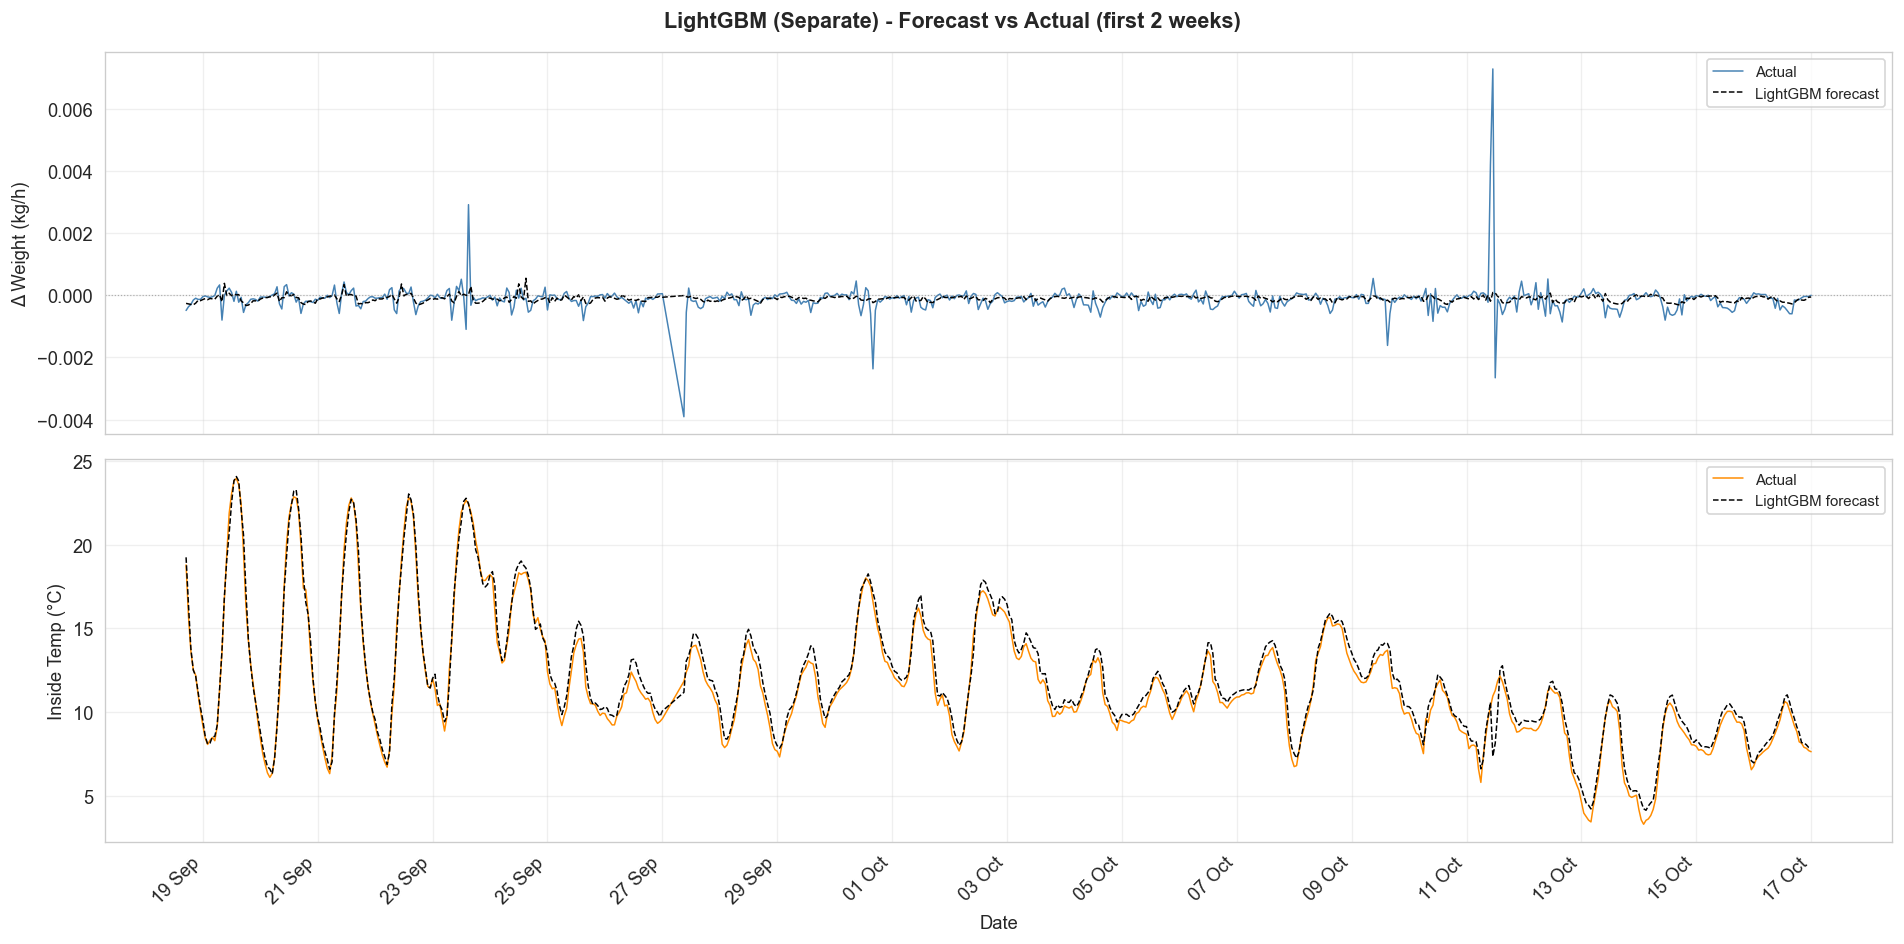
\includegraphics[width=\textwidth]{obrazky-figures/predpoved_lightGBM.png}
    \caption{Graf predikovaných a reálných hodnot pro oba modely LightGBM.}
    \label{fig:predpoved_lightGBM}
\end{figure}

\subsection*{Modely počítačového vidění}
Pro detekci objektů na česně úlu jsem vybrala tři architektury z~rodiny YOLO od společnosti Ultralytics: YOLOv8n, YOLO11n a YOLO26n, kde písmeno \textit{n} označuje variantu \textit{nano}. Volba těchto modelů vychází z~analýzy provedené v~kapitole \ref{sec:modely_detekce}. Obrázky z~datasetů byly rozděleny v~poměru 70:20:10 pro trénink, validaci a testování.

Trénování probíhalo ve dvou fázích. V~první fázi byl model YOLO26n natrénován na~komplexní sloučené datové sadě na serveru výzkumné skupiny KNOT (procesor Intel Core i7-14700K, 188,4 GiB RAM, grafická karta NVIDIA GeForce RTX 4090). Model pojmenovaný \textit{beekeeperv2} byl primárně určen k~nasazení, ale nejvíce jsem jej používala pro automatickou anotaci vlastních snímků.

Ve druhé fázi byly tři zvolené architektury natrénovány na každé ze dvou sestavených datových sad, čímž vzniklo celkem šest modelů. Jejich trénování probíhalo přímo prostřednictvím platformy Ultralytics (procesor AMD EPYC 9655, 1511 GB RAM, grafická karta NVIDIA RTX PRO 4500 Blackwell Server Edition a NVIDIA RTX PRO 6000 Blackwell Server Edition). Výsledky všech modelů shrnuje tabulka \ref{tab:trenovani_modelu}.

\begin{table}[H]
    \centering
    \begin{tabular}{|l|c|c|c|c|>{\centering\arraybackslash}p{2,3cm}|}
        \hline
        \textbf{Model} & \textbf{Sada} & \textbf{Přesnost} & \textbf{Úplnost} & \textbf{mAP@0.5} & \textbf{mAP@0.50--0.95} \\
        \hline
        beekeeperv2\,\footnotemark[1] & komplexní & 81,8\,\% & 78,3\,\% & 83,3\,\% & 54,2\,\% \\
        \hline
        \hline
        merged\_yolo8\,\footnotemark[1] & komplexní & 80,3\,\% & 80,4\,\% & 84,9\,\% & 59,3\,\% \\
        \hline
        merged\_yolo11\,\footnotemark[1] & komplexní & 82,6\,\% & 77,0\,\% & 83,9\,\% & 58,7\,\% \\
        \hline
        merged\_yolo26\,\footnotemark[1] & komplexní & 83,5\,\% & 78,0\,\% & 84,8\,\% & 60,7\,\% \\
        \hline
        my\_bees\_yolo8\,\footnotemark[1] & vlastní & 84,7\,\% & 83,1\,\% & 88,7\,\% & 65,6\,\% \\
        \hline
        my\_bees\_yolo11\,\footnotemark[1] & vlastní & 82,9\,\% & 85,0\,\% & 89,4\,\% & 66,5\,\% \\
        \hline
        my\_bees\_yolo26\,\footnotemark[1] & vlastní & 86,9\,\% & 79,0\,\% & 86,4\,\% & 63,6\,\% \\
        \hline
    \end{tabular}
    \caption{Srovnání výsledků trénování modelů počítačového vidění.}
    \label{tab:trenovani_modelu}
\end{table}

\footnotetext[1]{Více informací o~modelech lze najít zde: \url{https://platform.ultralytics.com/eliska-kremenkova/beekeeper5cvmodels}}

Z~výsledků je patrné několik zajímavých závěrů. Modely trénované výhradně na~vlastních snímcích dosahují konzistentně vyšších hodnot mAP@0.5 než modely trénované na~rozšířené sadě, a to navzdory výrazně menšímu počtu trénovacích snímků. Modely trénované na větší datové sadě naopak pracují s více třídami (včetně vosy a sršně), což je výhodou pro nasazení v~situacích, kdy se tyto druhy na česně skutečně vyskytují.

Pro nasazení na Raspberry Pi 5 jsem proto zvolila model my\_bees\_yolo11, protože dosáhl nejvyšší hodnoty mAP@0.5 (89,4\,\%) a zároveň nejlepší úplnosti ze všech testovaných modelů. Model byl exportován ve formátu NCNN optimalizovaném pro inferenci na~zařízeních bez GPU, jako je Raspberry Pi.

\section{Ukládání dat, síťová komunikace a softwarové řešení}
Datový tok systému lze rozdělit do několika fází: sběr dat ze senzorů i kamery, přenos prostřednictvím bezdrátové sítě, příjem a uložení na serverové straně, a periodická predikce a detekce anomálií.

\subsection*{Firmware senzorové jednotky (ESP32-S3)}
Firmware senzorové jednotky byl vyvinut v~prostředí Arduino IDE v~jazyce C++ a zajišťuje tři souběžné funkce: čtení dat ze senzorů, jejich lokální zobrazení na displeji a periodické odesílání prostřednictvím protokolu MQTT.

Čtení a zobrazení dat probíhá každé 2 sekundy, čímž je zajištěna plynulá aktualizace lokálního zobrazení bez závislosti na síťovém připojení. Na displeji jsou zobrazeny aktuální hodnoty všech měřených veličin a stavové indikátory Wi-Fi a MQTT připojení (zelená při~aktivním spojení, červená při výpadku). Odesílání dat probíhá v~intervalu 5 minut, který byl zvolen jako kompromis mezi dostatečným časovým rozlišením pro sledování pomalu se měnících veličin a minimalizací počtu síťových operací a energetické náročnosti zařízení. Tento interval je srovnatelný s~komerčními řešeními (viz tabulka \ref{tab:porovnani_komercnich_produktu}).

Před odesláním jsou hodnoty hmotnosti filtrovány pomocí exponenciálního klouzavého průměru (EMA, Exponential Moving Average) s~koeficientem $\alpha = 0{,}2$. Samotná funkce \texttt{read\_average(5)} knihovny HX711 již interně průměruje 5 po sobě jdoucích hodnot ADC převodníku, čímž eliminuje vysokofrekvenční šum a ojedinělé výrazné odlehlé hodnoty způsobené například otřesy. EMA následně zajišťuje plynulé přechody mezi měřeními a potlačuje krátkodobé výkyvy při zachování schopnosti sledovat skutečné změny hmotnosti. Nižší hodnota $\alpha$ by způsobovala přílišnou setrvačnost modelu a pomalou reakci na náhlé změny, jako je například rojení, a vyšší hodnota by naopak propouštěla více šumu.

Data jsou odesílána jako JSON objekt:
\begin{verbatim}
    {"weight":41.2,"t_o":23.6,"t":35.4,"h":52,"p":984.1}
\end{verbatim}
kde \texttt{weight} označuje hmotnost úlu v~kg, \texttt{t\_o} venkovní teplotu ze senzoru DS18B20 ve\,°C, \texttt{t} vnitřní teplotu ve\,°C, \texttt{h} relativní vlhkost v~\% a \texttt{p} atmosferický tlak naměřené senzorem BME280 v~hPa. Data jsou odesílána pouze tehdy, jsou-li dostupné hodnoty alespoň z~váhy a venkovního teplotního senzoru -- při chybě senzoru firmware odesílání přeskočí.

Firmware obsahuje mechanismy pro obnovu připojení: při výpadku Wi-Fi nebo MQTT spojení se zařízení opakovaně pokouší o~znovupřipojení, aniž by to blokovalo lokální zobrazení dat na displeji. Kalibraci váhy a tárování lze provést přes sériové rozhraní zasláním příkazu \texttt{t} (tare) nebo \texttt{c} (calibrate). Firmware zároveň obsahuje pevně uložené kalibrační hodnoty, konkrétně nulový offset (\texttt{offset\_raw}) a citlivost senzoru (\texttt{counts\_per\_kg}), které jsou načteny při každém spuštění. Váha je tak schopna okamžitě měřit i po výpadku napájení bez nutnosti manuální kalibrace.

\subsection*{Bee counter (Raspberry Pi 5)}
Skript \texttt{bee\_counter.py} běžící na Raspberry Pi 5 zajišťuje kontinuální vizuální analýzu letáku. Kamera snímá záběr s~rozlišením 2304~$\times$~1296 pixelů při 15 snímcích za sekundu s~ručně nastavenou polohou ostření (\texttt{LensPosition} = 5,0). Model YOLO11n ve formátu NCNN zpracovává každý snímek s~prahem spolehlivosti 0,4 a sleduje detekované objekty pomocí trackeru ByteTrack.

Logika počítání je založena na virtuální dělicí linii umístěné uprostřed záběru. Každý sledovaný jedinec, jehož trajektorie tuto linii překříží, je zaznamenán jako průchod dovnitř (\texttt{bees\_in}) nebo ven (\texttt{bees\_out}) z~úlu. Včely nesoucí pyl (\texttt{pollen\_in}) jsou evidovány pouze při průchodu dovnitř, jelikož pyl je do úlu přinášen, nikoli odnášen. Aby bylo zamezeno vícenásobnému započítání téhož jedince, je každé \texttt{track\_id} zaznamenáno nejvýše jednou a křížení je vyhodnoceno až po minimálně třech po sobě jdoucích snímcích, čímž se eliminují náhodné detekce.

Oproti přístupu použitému v~předchozí práci \cite{Chovancova2025}, kde bylo pro každou třídu objektů (včela, matka, vosa) nasazen samostatný model a analýza probíhala dávkově na nahraných a uložených třicetivteřinových videích, jsem zde zvolila odlišný přístup. Jediný model YOLO11n zpracovává obě třídy současně a inference probíhá snímek po snímku v~reálném čase bez nutnosti ukládání videa. Tento přístup eliminuje latenci způsobenou nahráváním a dávkovým zpracováním, snižuje nároky na úložný prostor a umožňuje kontinuální sledování letáku bez přerušení.

Počty jsou akumulovány v~rámci nastavitelného intervalu a po jeho uplynutí odeslány jako JSON zpráva na MQTT broker na Raspberry Pi 4. Na rozdíl od senzorových dat, u nichž případný výpadek znamená pouze chybějící vzorek, který lze případně rekonstruovat, jsou chybějící záznamy o~průchodech včel nenávratně ztraceny. Z~toho důvodu je každý průchod zapsán do lokálního CSV souboru, který slouží jako záloha pro případ výpadku sítě.

\subsection*{Přenos dat -- protokol MQTT a Wi-Fi}
Oba zdrojové uzly (ESP32-S3 a Raspberry Pi 5) odesílají data jako JSON zprávy přes protokol MQTT na broker Eclipse Mosquitto verze 2.x, spuštěný jako systémová služba na~Raspberry Pi 4. Senzorová data jsou publikována na téma \texttt{beehive/hive1/sensors}, data z~kamerového modulu na téma \texttt{beehive/hive1/camera}. Oba uzly využívají úroveň kvality QoS 0, protože případná ztráta jednoho vzorku v~pětiminutovém nebo delším intervalu není pro účely monitorování kritická a vyšší úrovně by zbytečně zvyšovaly režii komunikace.

\subsection*{Příjem a ukládání dat na Raspberry Pi 4}
Na Raspberry Pi 4 běží jako \textit{systemd} služba skript \texttt{subscriber.py} v~jazyce Python, který se přihlásí k~odběru obou MQTT témat a přijatá data ukládá do databáze SQLite. Ta~obsahuje tabulky: \texttt{readings} pro senzorová data (časová značka, hmotnost, t\_o, t, h, p) a \texttt{camera\_readings} pro data z~kamerového modulu (časová značka, bees\_in, bees\_out, pollen\_in). SQLite jsem zvolila proto, že nevyžaduje samostatně běžící databázový server a celou databázi ukládá do jediného souboru, což zjednodušuje zálohování i přenositelnost dat. Registrace jako \textit{systemd} služba zajišťuje automatické spuštění po startu systému a restart při neočekávaném pádu procesu.

\subsection*{Predikce a detekce anomálií}
Skript \texttt{forecast\_anomaly\_detection.py} je spouštěn každých 15 minut prostřednictvím plánovače \textit{cron}. Při každém spuštění načte posledních 172 hodin senzorových dat z~databáze, navzorkuje je na hodinové intervaly a sestaví příznakovou matici totožnou s~tou použitou při trénování -- tedy zpožděné hodnoty pro offsety 1, 2, 3, 6, 12, 24, 48 a 168 hodin, klouzavé průměry a směrodatné odchylky v~oknech 24 a 168 hodin a cyklické kalendářní příznaky. Načte oba natrénované modely LightGBM a provede predikci pro nejaktuálnější dostupný hodinový vzorek.

Anomálie jsou detekovány reziduální metodou: pro každou cílovou veličinu je vypočteno reziduum (rozdíl skutečné a predikované hodnoty), které je porovnáno s~historickými reziduálními hodnotami dostupnými v~aktuálním okně dat. Časový krok je označen jako anomální, pokud absolutní odchylka reziduí překročí práh $\pm5\sigma$. Pro hmotnost je navíc vyžadováno, aby absolutní hodnota rezidua přesáhla 0,5 kg -- tato podmínka zabraňuje falešným poplachům způsobeným omezeným rozlišením tenzometru (20 gramů). Výsledky predikce i příznak anomálie jsou uloženy do tabulky \texttt{predictions} v~rámci stejné SQLite databáze.

\section{Grafické uživatelské rozhraní}
Pro vizualizaci dat jsem zvolila open-source platformu Grafana, která umožňuje tvorbu interaktivních dashboardů nad různými datovými zdroji. Jako zdroj dat je připojena lokální databáze SQLite prostřednictvím příslušného pluginu. Vzdálený přístup k~rozhraní je zajištěn sítí VPN Tailscale, která umožňuje bezpečné připojení k~Raspberry Pi 4 odkudkoliv.

Hlavní dashboard (viz obrázek \ref{fig:grafana_ui}) zobrazuje časové průběhy všech měřených veličin -- hmotnosti úlu, venkovní teploty, vnitřní teploty, relativní vlhkosti a atmosférického tlaku -- a umožňuje jejich sledování v~libovolném časovém okně. Součástí jsou také grafy predikce změny hmotnosti a vnitřní teploty, kde jsou predikovaná a skutečná hodnota zobrazeny v~jednom grafu pro přímé vizuální porovnání. Každý z~grafů lze doplnit o~zobrazení detekovaných anomálií prostřednictvím přepínačů \textit{Weight anomaly} a \textit{Inside temperature anomaly}. Ty jsou znázorněny jako svislé přerušované čáry v~časových okamžicích, kdy systém detekoval anomální chování.

\begin{figure}[H]
    \centering
    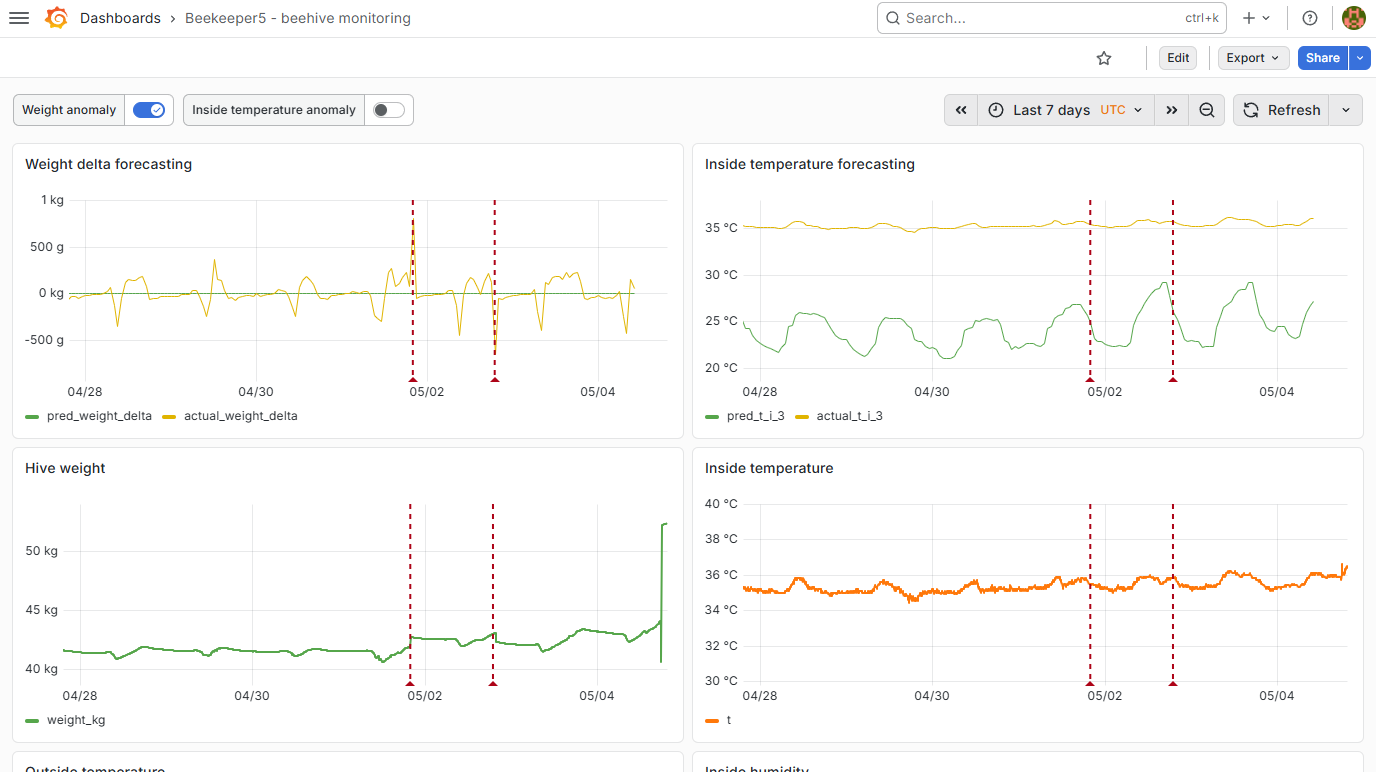
\includegraphics[width=\textwidth]{obrazky-figures/grafana_ui.png}
    \caption{Uživatelské rozhraní platformy Grafana.}
    \label{fig:grafana_ui}
\end{figure}

Další funkcí platformy Grafana je automatické upozorňování na detekované nežádoucí stavy. Pro tyto účely jsem nastavila dvě pravidla: jedno pro hmotnost a druhé pro vnitřní teplotu. Obě pravidla jsou vyhodnocována každou hodinu a při splnění podmínky je odesláno e-mailové upozornění na nakonfigurovanou adresu. Zpráva upozornění obsahuje stručný popis události a rozdílu mezi skutečnou a predikovanou hodnotou, aby měl včelař okamžitý přehled o~závažnosti anomálie.

Jednotka ESP32-S3 disponuje integrovaným displejem, který zobrazuje aktuální naměřené hodnoty všech veličin přímo na zařízení (viz obrázek \ref{fig:ESP32_displej}). Tato funkce je užitečná zejména při fyzické kontrole úlu na stanovišti, kdy včelař může okamžitě odečíst aktuální hmotnost, teplotu nebo vlhkost bez nutnosti otevírat mobilní aplikaci nebo notebook.

\begin{figure}[H]
    \centering
    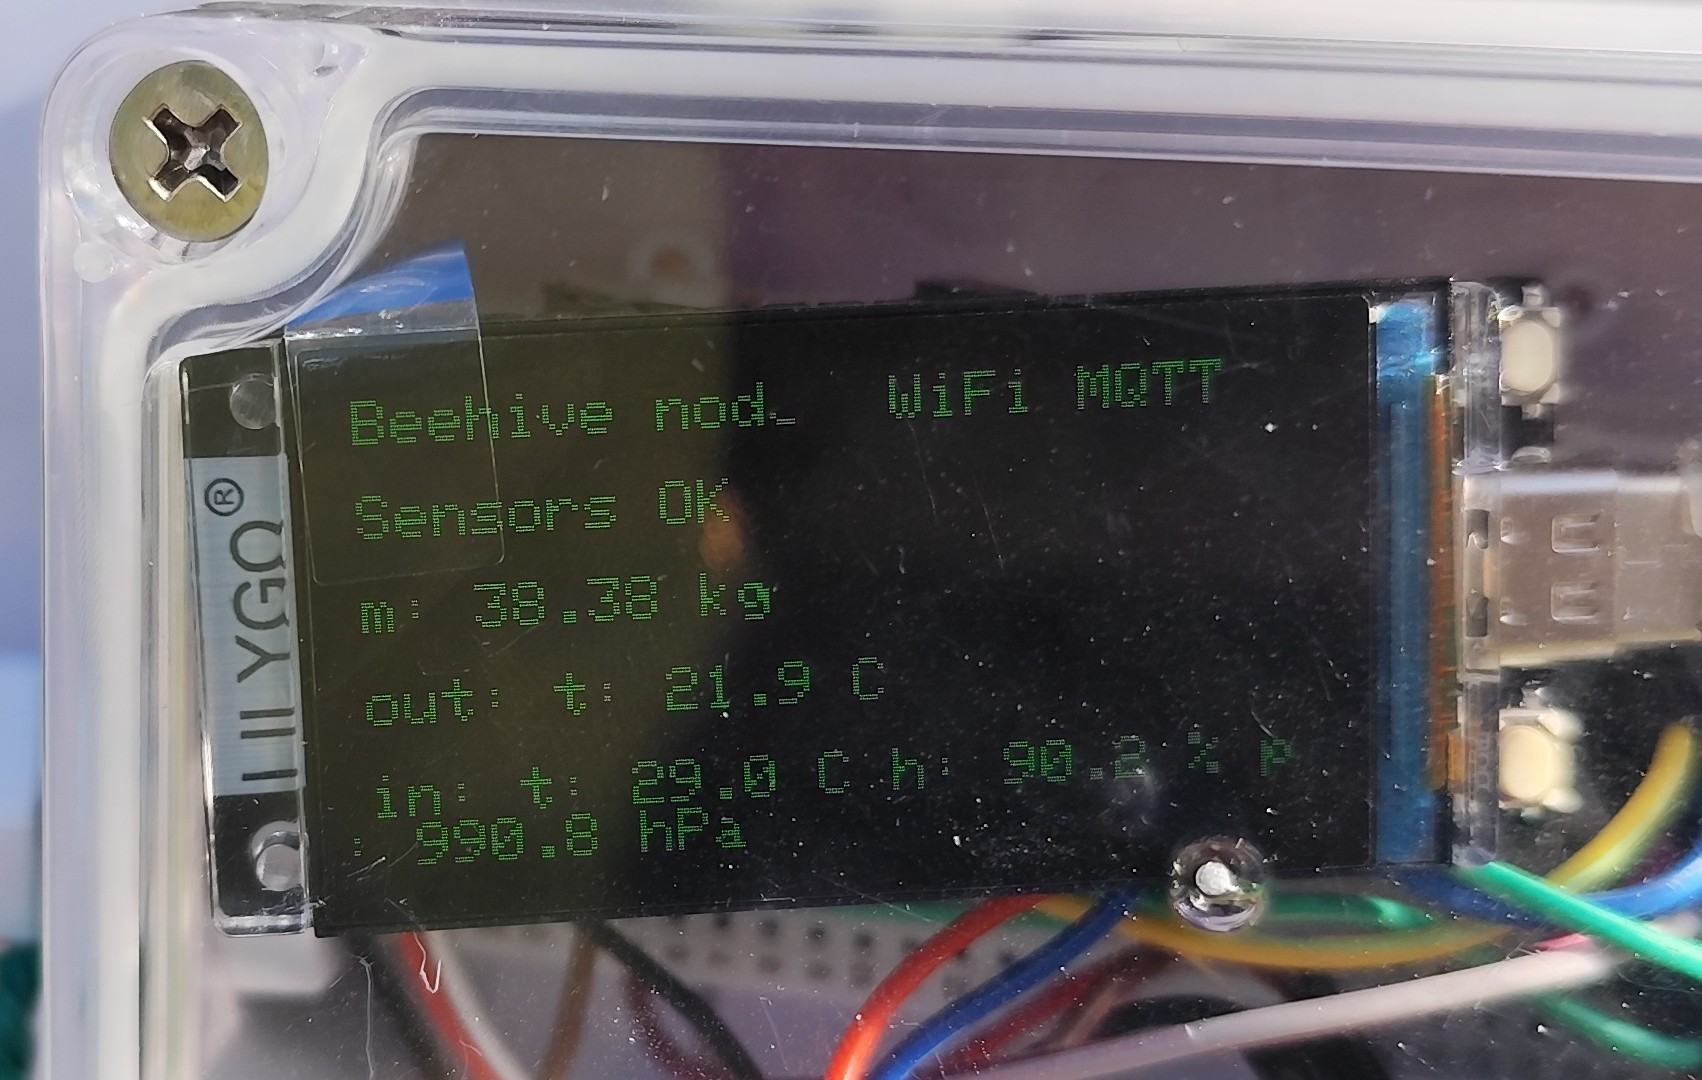
\includegraphics[width=0.5\textwidth]{obrazky-figures/ESP32_displej.jpg}
    \caption{Lokální zobrazení měření na integrovaném displeji ESP32-S3.}
    \label{fig:ESP32_displej}
\end{figure}

\chapter{Testování a nasazení systému}
Tato kapitola popisuje průběh nasazení systému v~reálných podmínkách a shrnuje výsledky testování jeho jednotlivých částí. Nejprve je popsán samotný průběh nasazení v~obou fázích vývoje, následně jsou analyzována data nasbíraná senzorovým modulem včetně ověření přesnosti váhy a funkčnosti detekce anomálií. Samostatná sekce je věnována testování kamerového modulu a výsledkům počítání včel. Závěr kapitoly tvoří srovnání navrženého systému s~vybranými existujícími řešeními a návrhy na budoucí vylepšení.

\section{Průběh nasazení}
Testování systému probíhalo na rodinném včelařském stanovišti ve Zlíně, kde je chováno sedm včelstev, přičemž monitorovací technika byla nasazena na jediném úlu. Testování probíhalo ve dvou fázích odpovídajících dvěma verzím hardwarového vybavení.

První verze systému, zahrnující senzorovou jednotku ESP32-S3 s~váhou, převodníkem HX711 a venkovním teplotním senzorem DHT11, byla nasazena 7. března 2026. Systém v~této konfiguraci fungoval až do 11. dubna 2026, tedy přibližně pět týdnů v~reálných venkovních podmínkách včetně mrazivých nocí a deštivého počasí, přičemž napájení zajišťovaly solární panel s~akumulátorem. V~průběhu tohoto období došlo k~několika krátkodobým výpadkům záznamu dat, které však nebyly způsobeny selháním senzorové jednotky, ale lidskou chybou -- Raspberry Pi 4 sloužící jako server byl v~těchto případech odpojen od~napájení.

Přechod na finální podobu systému s~přidaným vnitřním senzorem BME280 proběhl 18.~dubna 2026. Instalace vnitřního senzoru vyžadovala fyzické otevření úlu a umístění senzoru mezi rámky v~jeho horní části. Tento zásah bylo nutné odložit, dokud venkovní teploty nedosáhly hodnot bezpečných pro otevření úlu -- při nízkých teplotách hrozí včelstvu podchlazení plodu, které může mít pro kolonii fatální následky. Finální verze systému běží nepřetržitě\,\footnote{Ke dni 4. května 2026} od 18. dubna 2026.

\section{Senzorový modul a nasbíraná data}
Od nasazení finální verze systému 18. dubna 2026 nebyl zaznamenán jediný výpadek senzorové jednotky ani přerušení přenosu dat. Databáze obsahuje nepřetržitý záznam v~pětiminutovém intervalu bez chybějících hodnot, čímž byla ověřena spolehlivost jak samotného hardwaru, tak komunikačního řetězce ESP32-S3 $\rightarrow$ MQTT $\rightarrow$ Raspberry Pi 4 $\rightarrow$ SQLite. Celkový průběh hmotnosti úlu od nasazení finální verze je zobrazen na obrázku \ref{fig:grafana_hmotnost}.

\begin{figure}[H]
    \centering
    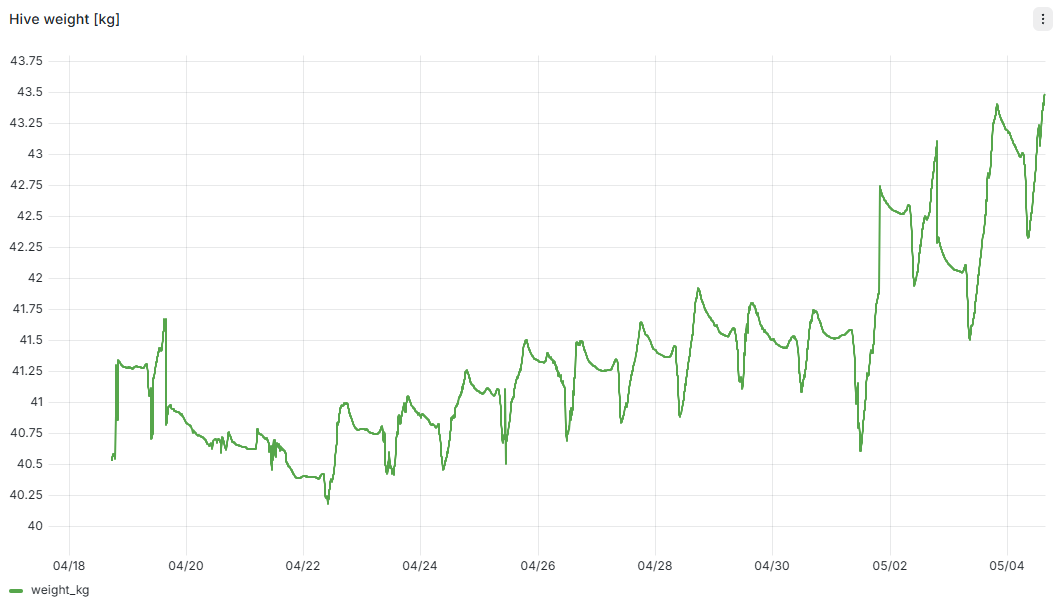
\includegraphics[width=\textwidth]{obrazky-figures/grafana_hmotnost.png}
    \caption{Průběh hmotnosti úlu v~období 18. dubna -- 5. května 2026.}
    \label{fig:grafana_hmotnost}
\end{figure}

\subsection*{Vnitřní teplota}
Dle dat (viz obrázek \ref{fig:grafana_vnitrni_teplota}) lze vidět, že je senzor BME280 umístěn v~bezprostřední blízkosti plodového hnízda, jelikož se teplota pohybuje v~rozsahu přibližně 34,5 až 36,5\,°C, což odpovídá správné teplotě plodového hnízda v~tomto období (podrobněji viz \ref{sec:veliciny}).

\begin{figure}[H]
    \centering
    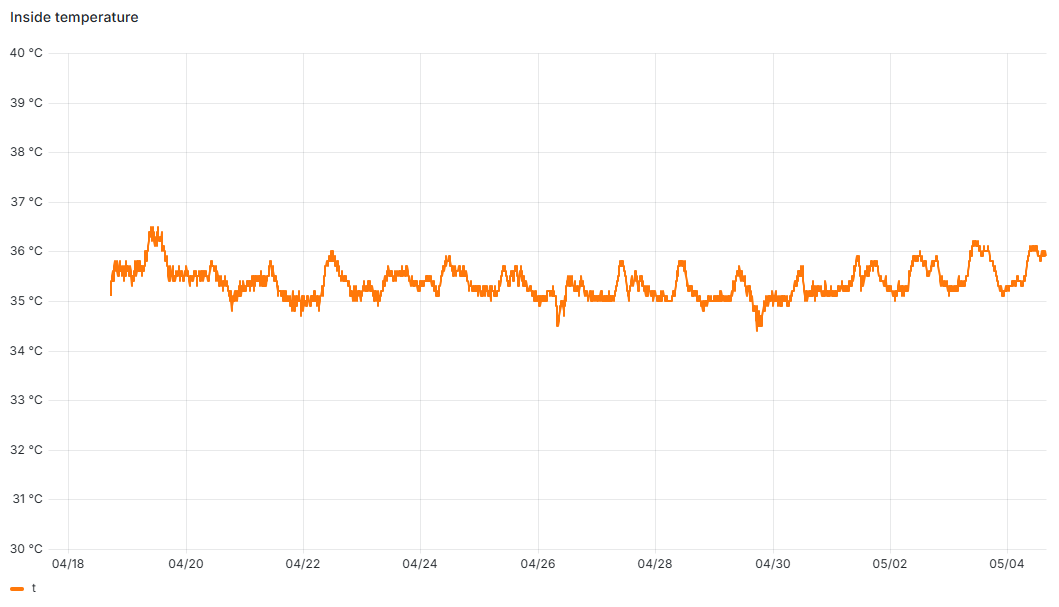
\includegraphics[width=\textwidth]{obrazky-figures/grafana_vnitrni_teplota.png}
    \caption{Průběh vnitřní teploty úlu v~období 18. dubna -- 5. května 2026.}
    \label{fig:grafana_vnitrni_teplota}
\end{figure}

Naměřené hodnoty jsou se výrazně liší s~daty z~datasetu BeeObserver \cite{BeeObserver}, v němž senzory DS18B20 umístěné uvnitř úlu mezi rámky vykazují v~jarních měsících hodnoty vnitřní teploty v~rozmezí 20 až 25\,°C. Ačkoliv dataset obsahuje i kolonie s~fyziologicky správnějšími hodnotami, musela jsem zvolit kompromis, jelikož většina z~nich disponuje příliš krátkým sledovaným obdobím či velkým množstvím chybějících hodnot, a proto nebyly pro trénování modelu zvoleny. Tento poznatek má přímý dopad na kvalitu dat použitých při trénování modelu pro predikci vnitřní teploty, a je proto jedním z~klíčových omezení.

\subsection*{Ověření přesnosti váhy a pozorovatelné události}
Přestože přesnost váhy nebyla ověřena formálním srovnáním s~kalibrovaným referenčním přístrojem, lze ji posoudit na základě dvou konkrétních zaznamenaných událostí se známou hmotností.

První událostí bylo krmení včelstva cukrovou pastou dne 9. dubna 2026 z~důvodu chladného počasí. Do úlu bylo přidáno 4 kg cukrové pasty, což se na záznamu váhy projevilo jako náhlý přírůstek odpovídající přibližně této hodnotě (viz obrázek \ref{fig:grafana_hmotnost_krmeni}). Tato událost pochází ještě z~období první verze systému, kdy byl nasazen venkovní senzor DHT11, ale váha již fungovala ve své finální podobě.

\begin{figure}[H]
    \centering
    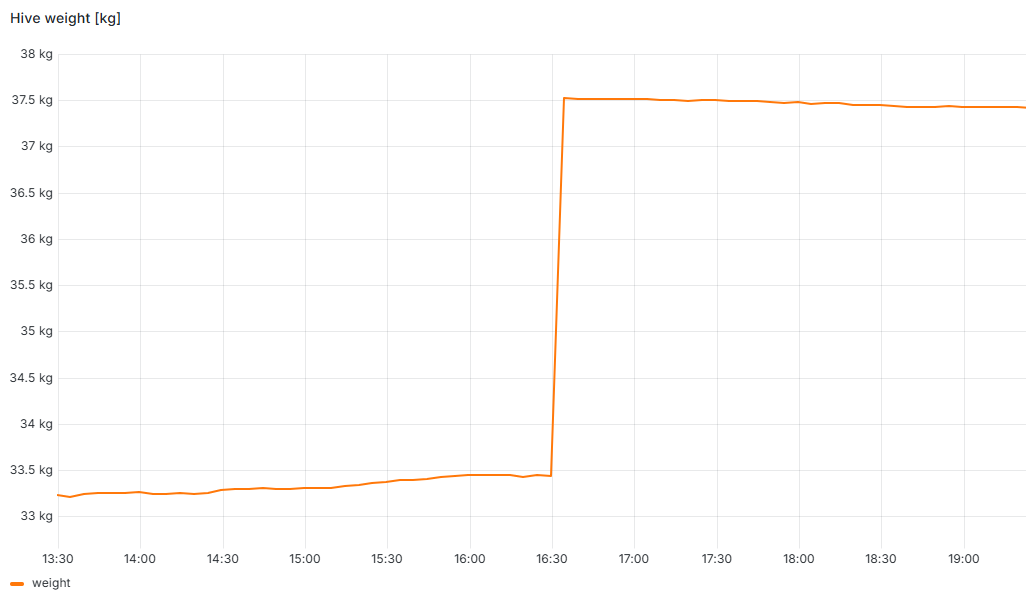
\includegraphics[width=\textwidth]{obrazky-figures/grafana_hmotnost_krmeni.png}
    \caption{Náhlý nárůst hmotnosti při krmení včel.}
    \label{fig:grafana_hmotnost_krmeni}
\end{figure}

Druhou a přesnější ověřovací událostí bylo nasazení kamerového modulu na úl večer 1.~května 2026. Hmotnost modulu činí 829 g. Na záznamu váhy je patrný přírůstek i následný úbytek odpovídající přibližně této hodnotě (viz obrázek \ref{fig:grafana_hmotnost_kamera}). Konkrétní hodnoty při odstranění modulu  byly:
\[43{,}1039 - 42{,}2807 = 0{,}8232\,kg\]
kde rozdíl od skutečnosti činí pouhých 6 g, což je v~kontextu monitorování hmotnosti úlu zanedbatelná odchylka.

\begin{figure}[H]
    \centering
    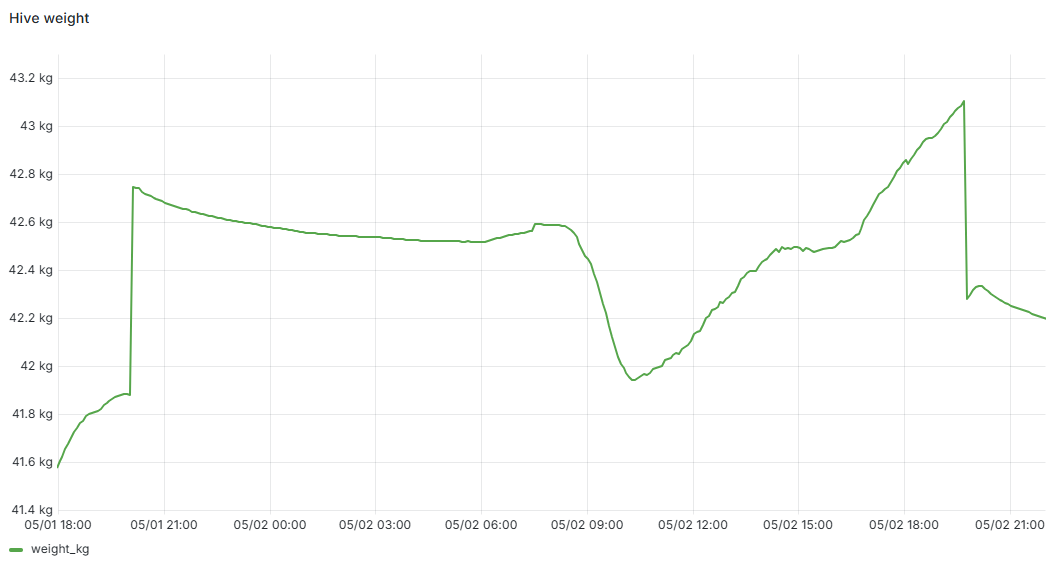
\includegraphics[width=\textwidth]{obrazky-figures/grafana_hmotnost_kamera.png}
    \caption{Náhlý nárůst a pokles hmotnosti při nasazení kamerového modulu.}
    \label{fig:grafana_hmotnost_kamera}
\end{figure}

Na delším časovém horizontu lze na záznamu váhy pozorovat také přirozené přírůstky hmotnosti v~průběhu dnů s~příznivým počasím, kdy včely aktivně sbírají nektar (viz obrázek~\ref{fig:grafana_hmotnost}). Tyto přírůstky jsou typicky v~řádu jednotek až desítek gramů za hodinu a tvoří charakteristický denní vzor -- hmotnost roste přes den a v~noci, kdy jsou včely v~úlu, lehce klesá v~důsledku spotřeby zásob a odpařování vody z~nektaru.

\subsection*{Detekce anomálií a upozornění včelaře}

\begin{figure}[H]
    \centering
    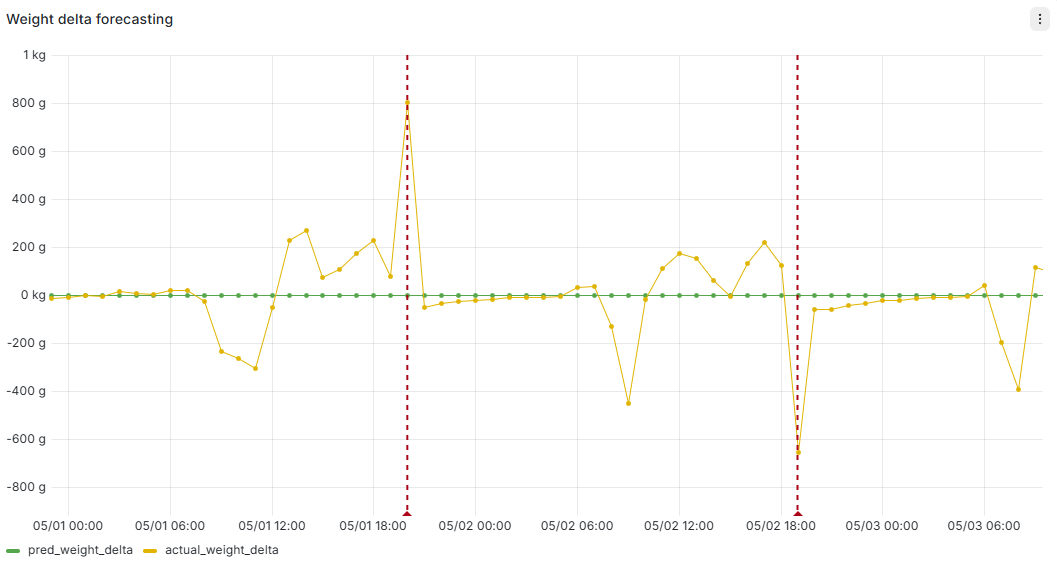
\includegraphics[width=\textwidth]{obrazky-figures/grafana_hmotnost_anomalie.png}
    \caption{Zachycení abnormální změny hmotnosti.}
    \label{fig:grafana_hmotnost_anomalie}
\end{figure}

Obě výše popsané události -- nasazení a odstranění kamerového modulu -- byly systémem automaticky detekovány jako anomálie (viz obrázek~\ref{fig:grafana_hmotnost_anomalie}). Zároveň bylo na nakonfigurovanou e-mailovou adresu odesláno upozornění obsahující popis události a konkrétní hodnotu rozdílu hmotnosti (viz obrázek~\ref{fig:grafana_alert_email}).

\begin{figure}[H]
    \centering
    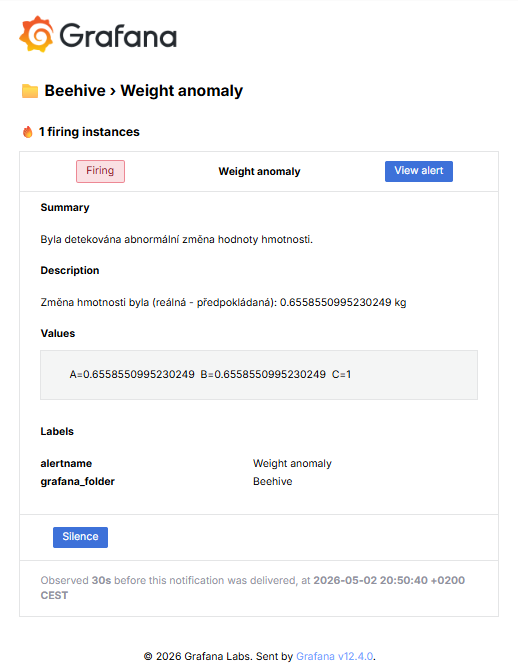
\includegraphics[width=0.7\textwidth]{obrazky-figures/grafana_alert_email.png}
    \caption{Zaslané upozornění včelaři prostřednictvím e-mailu.}
    \label{fig:grafana_alert_email}
\end{figure}

\subsection*{Predikce časových řad}
Jak je patrné z~grafu na obrázku \ref{fig:grafana_hmotnost_anomalie}, predikované hodnoty hmotnosti jsou blízko~0 (ve~skutečnosti se jedná o~setiny až tisíciny kilogramu za hodinu), zatímco skutečné naměřené hodnoty vykazují výrazně větší výkyvy. Příčinou tohoto chování je nesoulad mezi trénovacími a reálnými daty: model byl trénován na hodinově agregovaných datech z~datasetu BeeObserver, v němž jsou krátkodobé výkyvy vyhlazeny průměrováním, zatímco vlastní data jsem se rozhodla měřit v~pětiminutových intervalech, a proto obsahují více krátkodobé variability. Model se tedy naučil předpovídat vyhlazené hodinové změny a na pětiminutových datech systematicky podhodnocuje amplitudu výkyvů. Řešením by bylo přetrénování modelu přímo na datech nasbíraných vlastním systémem po delší dobu -- minimálně v~délce jedné vegetační sezóny -- aby model zachytil skutečnou dynamiku monitorovaného včelstva v~odpovídajícím časovém rozlišení.

\section{Napájení systému} \label{sec:napajeni_systemu}
Senzorová jednotka ESP32-S3 společně s~váhovým senzorem a oběma teplotními senzory je napájena výhradně ze solárního panelu a akumulátoru. Tento provozní režim byl ověřen v~průběhu téměř dvou měsíců, od 7. března do současnosti\,\footnote{Ke dni 4. května 2026}, a zahrnoval období s~minimálním slunečním svitem, nočními teplotami pod bodem mrazu i déštěm. Po celou tuto dobu nedošlo k~výpadku způsobenému vybitím akumulátoru, ačkoli formální měření výdrže baterie při úplném stínění nebylo provedeno. 

Raspberry Pi 5 zajišťující zpracování obrazu v~kamerovém modulu se ukázalo jako problematické z~hlediska napájení z~akumulátoru. PWM regulátor nabíjení disponuje USB výstupy s~maximálním výkonem 10 W, což pro spuštění Raspberry Pi 5 nestačí. Zařízení vyžaduje napájení 5 V~při 5 A, což odpovídá výkonu 25 W. Kamerový modul je proto nutné napájet ze síťového zdroje, což jej v~současné podobě omezuje na stanoviště s~přístupem k~elektrické síti. 

\section{Kamerový modul a bee counter}
\subsection*{Volba tříd detekčního modelu}
Původní záměr zahrnoval nasazení komplexního modelu schopného rozlišovat pět tříd objektů -- standardní včelu, včelu nesoucí pyl, včelí matku, vosu a sršeň. Na základě konzultace s~praktikujícím včelařem a předběžného testování byl však tento záměr přehodnocen ve prospěch zjednodušeného modelu pracujícího pouze se dvěma třídami.

Hlavním důvodem je biologická povaha sledovaných objektů. Včelí matka zdravé kolonie úl prakticky neopouští -- výjimkou je oplodňovací let nově vylíhlé matky, při němž je však matka štíhlá a pohyblivá, rozměrově blízká dělnici. Typické obrazové datasety naopak zachycují vykrmenou plodící matku, jejíž rozměry jsou výrazně větší. Tento nesoulad mezi trénovacími daty a reálným výskytem na česně by vedl k~chybným detekcím.

Co se týká vetřelců, zdravé a silné včelstvo si vstup do úlu dokáže účinně hlídat. Ojedinělé vosy jsou zpravidla zlikvidovány strážními včelami dříve, než by se dostaly do~záběru kamery. Průchod jsem navíc navrhla tak, aby jím sršeň evropská nedokázala projít. Nejčastějšími \uv{vetřelci} jsou přitom včely samotné pocházející z~vedlejších kolonií -- ty jsou však z~pohledu monitorování nerozlišitelné od domácích včel.

Tato rozhodnutí byla ověřena i praktickým testováním. Při předběžném nasazení komplexního modelu (30. dubna 2026) byly opakovaně detekovány 1--4 vosy při prakticky nulovém počtu napočítaných včel (viz tabulka \ref{tab:komplexni_model_test}), což dokládá vysokou míru falešných poplachů způsobenou chybnou klasifikací včel jako vos. Přechod na model trénovaný výhradně na vlastních datech se dvěma třídami tyto falešné detekce eliminoval.

\begin{table}[H]
    \centering
    \begin{tabular}{|c|c|c|c|c|c|c|}
        \hline
        \textbf{Čas} & \textbf{bees\_in} & \textbf{bees\_out} & \textbf{pollen\_in} & \textbf{queen} & \textbf{wasp} & \textbf{hornet} \\
        \hline
        09:46:35 & 0 & 0 & 0 & 0 & 4 & 0 \\
        \hline
        09:46:47 & 0 & 0 & 0 & 0 & 4 & 0 \\
        \hline
        09:51:58 & 0 & 0 & 0 & 0 & 3 & 0 \\
        \hline
        09:57:19 & 0 & 0 & 0 & 0 & 0 & 0 \\
        \hline
        10:50:16 & 1 & 0 & 0 & 0 & 0 & 0 \\
        \hline
        10:55:41 & 0 & 0 & 0 & 0 & 1 & 0 \\
        \hline
        15:14:38 & 0 & 0 & 0 & 0 & 0 & 0 \\
        \hline
        15:15:38 & 0 & 0 & 0 & 0 & 0 & 0 \\
        \hline
        15:16:38 & 2 & 0 & 0 & 0 & 0 & 0 \\
        \hline
        15:17:38 & 3 & 0 & 0 & 0 & 2 & 0 \\
        \hline
        15:18:38 & 4 & 0 & 0 & 0 & 2 & 0 \\
        \hline
        15:19:33 & 4 & 1 & 0 & 0 & 3 & 0 \\
        \hline
    \end{tabular}
    \caption{Záznamy z~testování komplexního modelu dne 30. dubna 2026.}
    \label{tab:komplexni_model_test}
\end{table}

\subsection*{Průběh testování}
Testování kamerového modulu s~finálním modelem YOLO11n probíhalo 2. května 2026 v~době od 8:12:28 do 19:30:29, tedy přibližně 11 hodin a 18 minut. Testovací den byl slunečný s~venkovní teplotou nad 20\,°C (nejvyšší naměřená teplota dosáhla 27,1\,°C), tedy v~podmínkách vysoké letové aktivity včelstva, které představují pro detekční systém nejvyšší zátěž.

Kamera snímala záběr při cílové frekvenci 15 FPS. Při vysoké letové aktivitě včelstva v~průběhu dne však Raspberry Pi 5 z~důvodu tepelného omezení (throttlingu) provozní frekvenci snižovalo -- reálně dosahovaná snímková frekvence se pohybovala v~rozmezí 7,5 až 8,5 FPS. Průměrná provozní teplota procesoru činila 85\,°C, maximální pak 87,8\,°C. Takovou teplotu jsem díky zkušenostem z~předchozí práce \cite{Chovancova2025} nevyhodnotila jako nebezpečnou. Přestože throttling snižoval výpočetní výkon, dosahovaná frekvence 8 FPS se pro účely počítání včel ukázala jako dostatečná, jak dokládají výsledky uvedené níže.

Algoritmus ByteTrack sledoval v~průběhu testování průměrně 20--30 aktivních tras současně, maximální počet dosáhl 50 souběžně sledovaných jedinců.

\subsection*{Výsledky počítání včel}
Celkové výsledky počítání za celé testovací období shrnuje tabulka \ref{tab:testovani_bee_counter}.

\begin{table}[H]
    \centering
    \begin{tabular}{|l|r|}
    \hline
        \textbf{Veličina} & \textbf{Hodnota} \\
        \hline
        Včely přilétající do úlu (\texttt{bees\_in}) & 24 535 \\
        \hline
        Včely odlétající z~úlu (\texttt{bees\_out}) & 20 360 \\
        \hline
        Z~toho včely nesoucí pyl (\texttt{pollen\_in}) & 228 \\
        \hline
        Podíl pylových včel & 0,93\,\% \\
        \hline
        Doba měření & 11 hod 18 min \\
        \hline
    \end{tabular}
    \caption{Celkové výsledky počítání včel za testovací den 2. května 2026.}
    \label{tab:testovani_bee_counter}
\end{table}

Časový průběh počtů průchodů je zobrazen na obrázku \ref{fig:testovani_graf_aktivity}. Z~grafu je patrný charakteristický denní vzor letové aktivity -- nízká aktivita v~ranních hodinách, nárůst dopoledne s~kulminací v~nejteplejší části dne a postupný pokles k~večeru.

\begin{figure}[H]
    \centering
    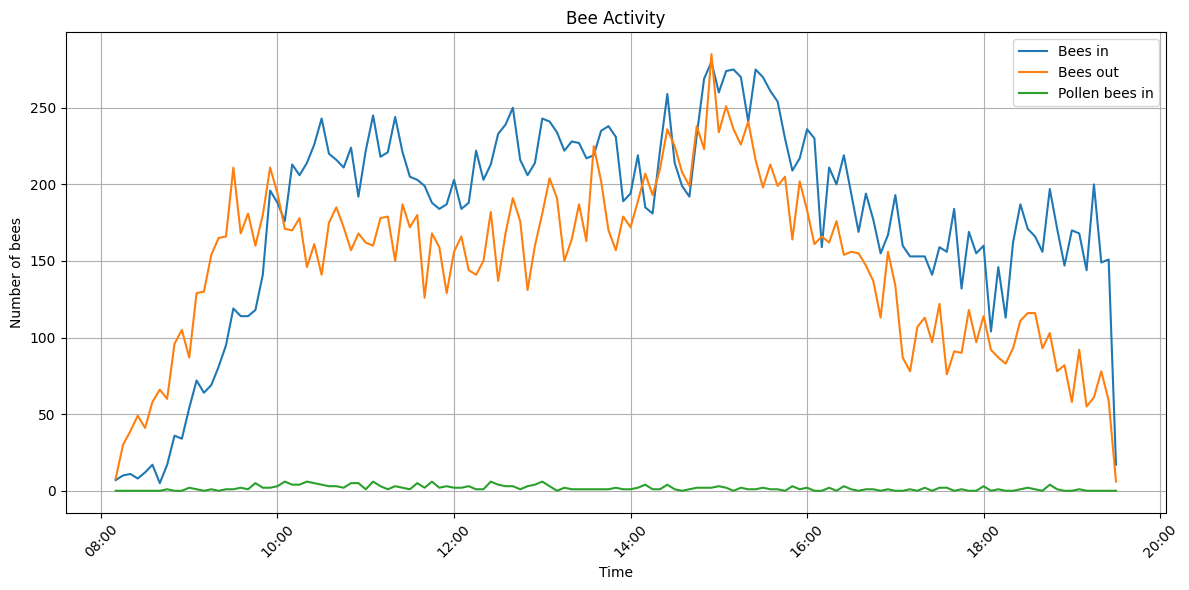
\includegraphics[width=\textwidth]{obrazky-figures/testovani_graf_aktivity.png}
    \caption{Graf letové aktivity včel z~testování dne 2. května 2026.}
    \label{fig:testovani_graf_aktivity}
\end{figure}

Zaznamenaný rozdíl mezi počtem přiletělých (24 535) a odletělých (20 360) včel činí přibližně 4 000 průchodů. Tento rozdíl není způsoben tím, že by dané množství včel zůstalo večer venku -- měření bylo ukončeno po západu slunce, kdy se včely vracejí do úlu. Příčinou je pravděpodobně asymetrie v~úspěšnosti detekce a sledování jedinců pohybujících se různou rychlostí: včely vracející se do úlu (\texttt{bees\_in}) nesou nektar nebo pyl a pohybují se výrazně pomaleji než včely odlétající (\texttt{bees\_out}), které úl opouštějí rychle. Pomalejší pohyb umožňuje algoritmu ByteTrack spolehlivěji udržet kontinuitu trasy přes dělicí linii, zatímco rychle letící jedinci mohou být sledováni přerušovaně a jejich průchod nemusí být zaznamenán vůbec. 

Počet zaznamenaných včel nesoucích pyl (\texttt{pollen\_in}) činí 228, což představuje pouhých 0,93\,\% z~celkového počtu přiletělých včel. Toto číslo je výrazně nižší, než by odpovídalo realitě -- v~době aktivní snůšky za slunečného dne lze očekávat, že značná část vracejících se jedinců nese pyl. Nepřímým dokladem aktivní snůšky je průběh hmotnosti úlu v~průběhu testovacího dne (viz obrázek \ref{fig:testovani_hmotnost}), kde je patrný nárůst o~více než 1 kg mezi ranními a odpoledními hodinami. Příčinou podhodnocení počtu pylových včel je pravděpodobně omezená kvalita obrazu při vysoké letové aktivitě v~kombinaci s~proměnlivými světelnými podmínkami, kdy jsou pylové košíčky na zadních nožkách včel v~záběru obtížně rozlišitelné. Třída \textit{pollen bee} tak představuje náročnější detekční úlohu než třída \textit{bee} a její spolehlivá detekce by pravděpodobně vyžadovala vyšší rozlišení kamery nebo stabilnější osvětlení sledované oblasti.

\begin{figure}[H]
    \centering
    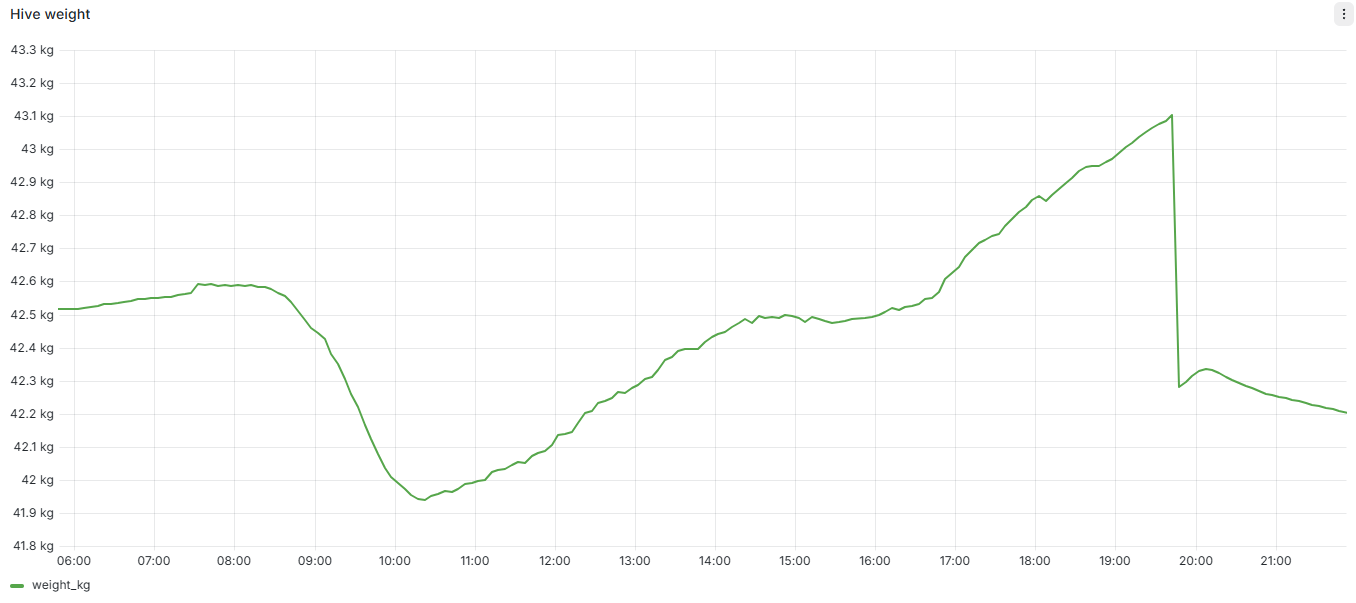
\includegraphics[width=\textwidth]{obrazky-figures/testovani_hmotnost.png}
    \caption{Průběh hmotnosti úlu v~testovací den 2. května 2026.}
    \label{fig:testovani_hmotnost}
\end{figure}

\subsection*{Kvalita detekce modelu}
Kromě samotného počítání průchodů byla ověřena i schopnost modelu detekovat včely ve~statickém záběru při vysoké hustotě jedinců. Na snímku pořízeném při vysoké letové aktivitě model YOLO11n detekoval 75 včel s~hodnotami spolehlivosti (\textit{confidence}) v~rozmezí 0,30 až 0,91 (viz obrázek \ref{fig:vysoka_aktivita_detekce}). Většina detekcí dosahovala confidence výrazně nad hodnotou 0,5, přičemž nejspolehlivěji byli detekováni izolovaní jedinci s~hodnotami okolo 0,90. Nižší hodnoty confidence se vyskytovaly zejména u~překrývajících se jedinců v~dolní části záběru, kde hustota včel ztěžuje přesnou lokalizaci hranic jednotlivých objektů.

\begin{figure}[H]
    \centering
    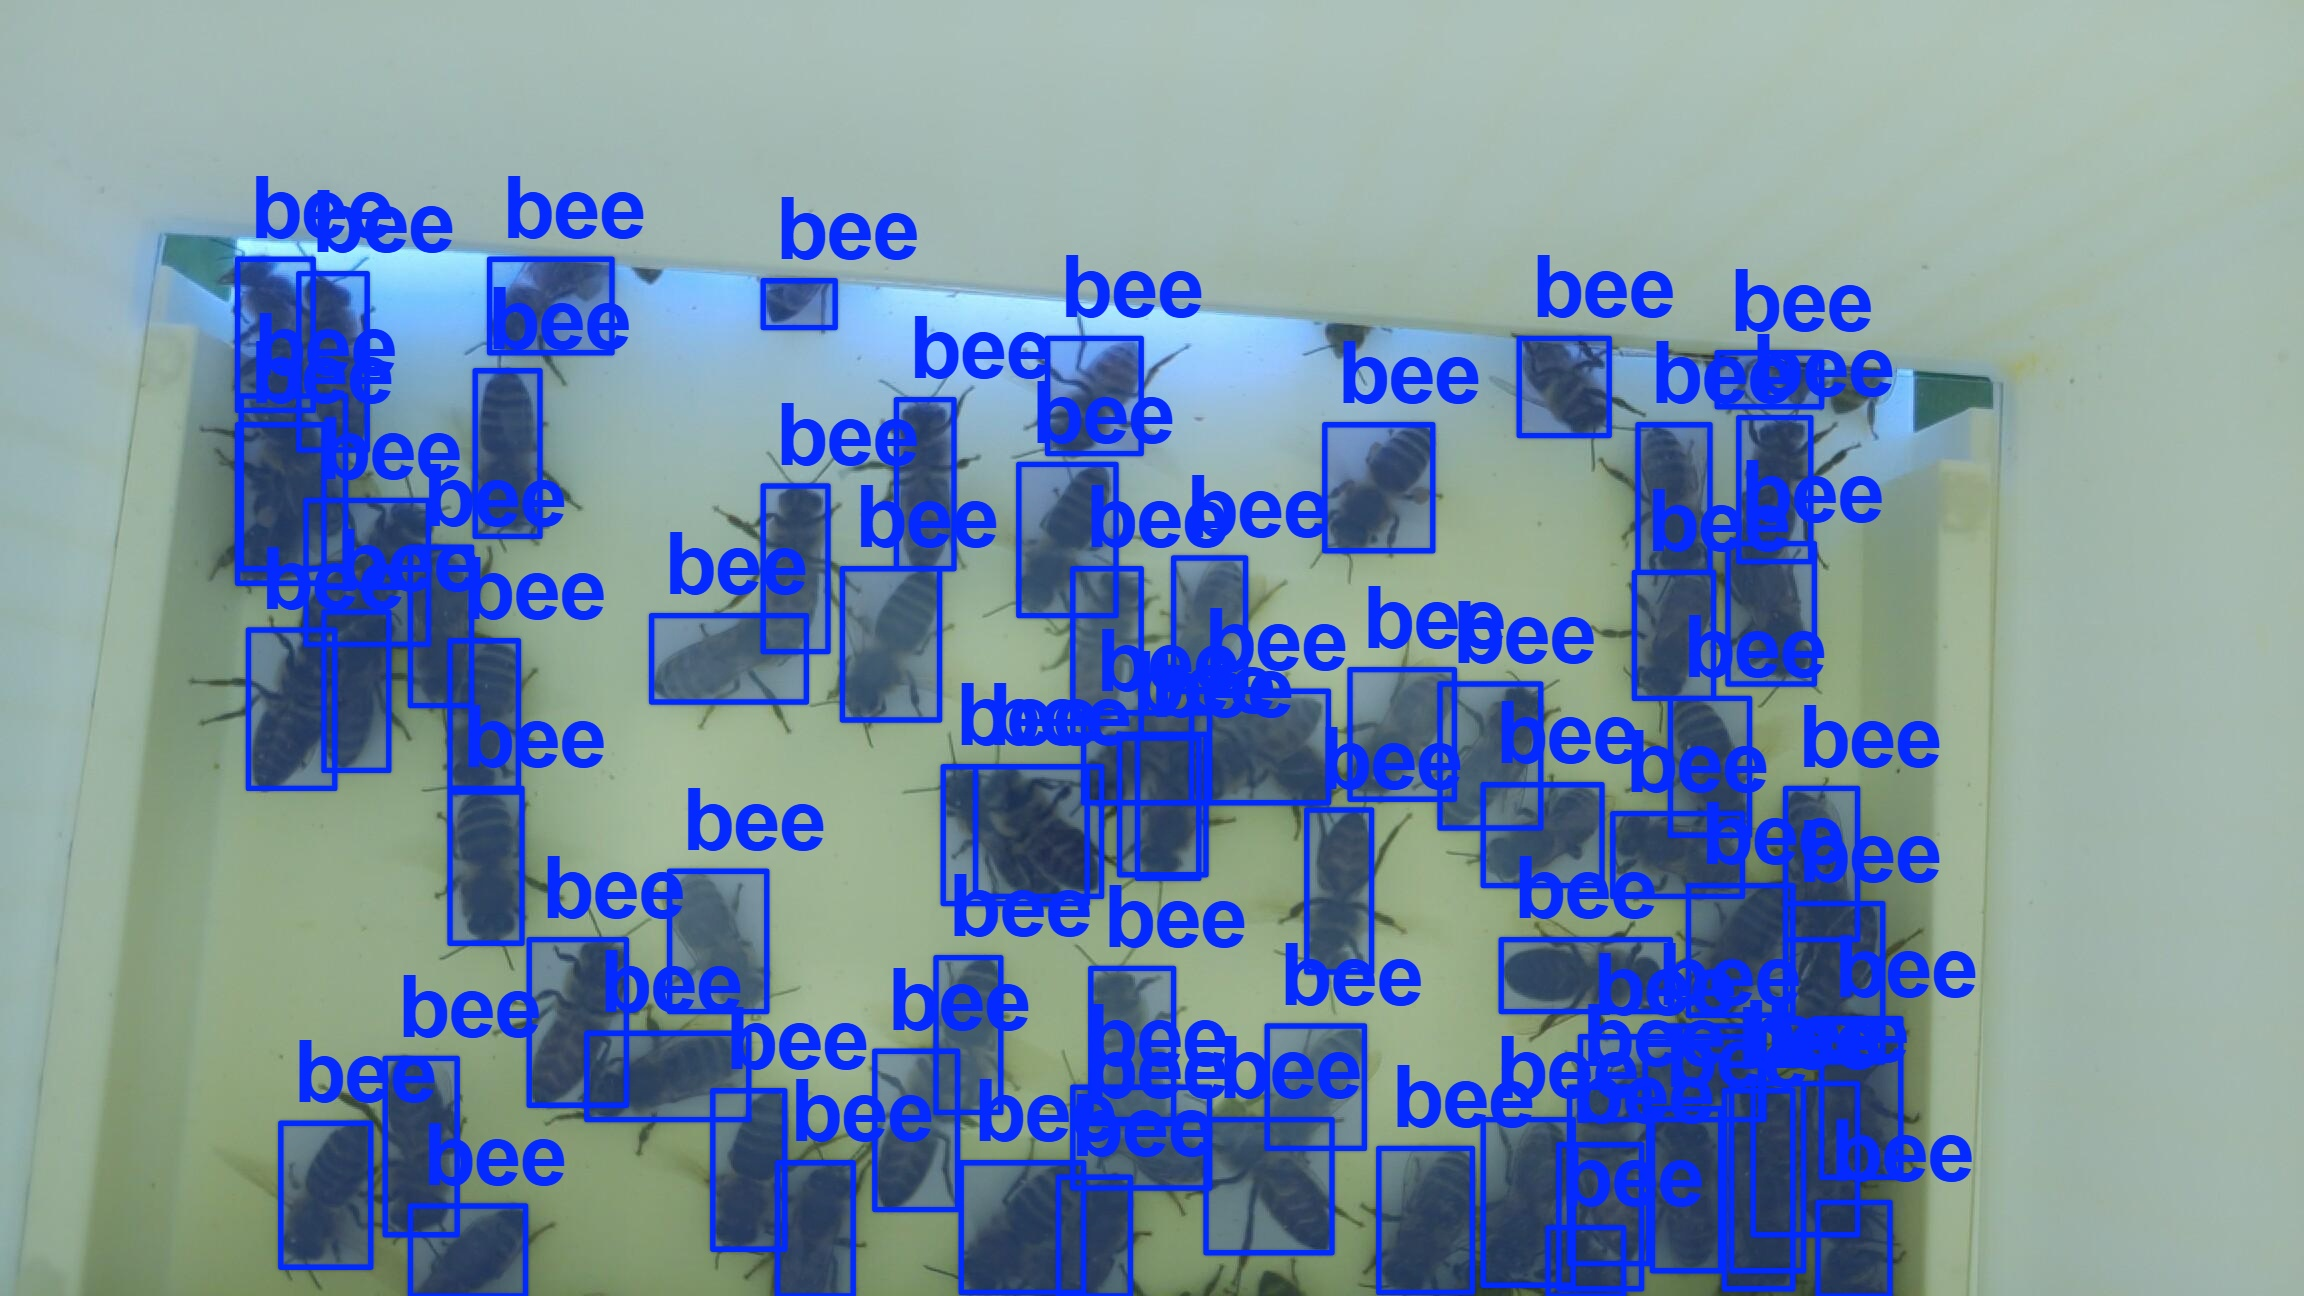
\includegraphics[width=0.7\textwidth]{obrazky-figures/vysoka_aktivita_detekce.jpg}
    \caption{Ukázka detekce modelu YOLO11n při vysoké hustotě včel na latáku.}
    \label{fig:vysoka_aktivita_detekce}
\end{figure}

Tento výsledek je překvapivý zejména s~ohledem na to, že snímek zachycuje podmínky výrazně náročnějšínež ty, na kterých byl model trénován -- trénovací snímky jsem záměrně filtrovala tak, aby obsahovaly pouze snímky s~minimálně se překrývajícími jedinci. 

\section{Srovnání s~některými z~existujících řešení}
Navržený systém lze srovnat jak s~komerčními produkty popsanými v~kapitole \ref{sec:komercni_reseni}, tak s~akademickými pracemi zaměřenými na kamerové monitorování včelstev. Přehled klíčových vlastností je uveden v~tabulce \ref{tab:srovnani_systemu}.

Z~tabulky je patrné, že navržený systém jako jediný kombinuje senzorové měření fyzikálních veličin s~kamerovým monitorováním česna. Oproti komerčním produktům přináší možnost klasifikace včel nesoucích pyl a jejich počítání. Naopak postrádá GPS modul pro~ochranu před krádeží, který nabízí například ApiVčelař, a umožňuje komunikaci pouze prostřednictvím Wi-Fi sítě. 

Při srovnání s~předchozí prací Bc. Chovancové \cite{Chovancova2025} je zřejmé, že obě řešení přistupují k~problematice odlišně a vzájemně se doplňují. Předchozí práce se zaměřuje výhradně na~kamerový modul a detekci širšího spektra objektů -- konkrétně včely, matky a vosy -- avšak bez senzorového monitorování fyzikálního stavu včelstva. Mé řešení naopak přidává senzorový modul, predikci časových řad a detekci anomálií, ale kamerový modul zjednodušuje na~dvě třídy (\textit{bee} a \textit{pollen bee}). Plnohodnotné sloučení obou přístupů -- tedy systém detekující vosy, matku i pylové včely a zároveň monitorující fyzikální veličiny s~využitím prediktivní analýzy -- představuje přirozený směr dalšího vývoje.

Co se týká srovnání s~akademickým projektem Beemon \cite{Beemon2021}, navržený systém využívá modernější přístup k~detekci objektů prostřednictvím modelu YOLO11n namísto segmentace na základě obrysů, která je citlivá na změny osvětlení a překryvy jedinců. Navíc disponuje pokročilejší analytickou vrstvou -- predikce časových řad a detekce anomálií pomocí LightGBM jsou funkce, které systém Beemon nenabízí. Naopak Beemon odesílá data v~reálném čase každých přibližně 30 sekund prostřednictvím IoT platformy ThingsBoard, zatímco senzorový modul navrženého řešení odesílá data v~pětiminutovém intervalu, kamerový modul pak v~nastavitelném intervalu.

Přímé kvantitativní srovnání přesnosti detekce s~ostatními řešeními není možné, protože většina dostupných prací nezveřejňuje testovací protokoly nebo využívá odlišné metriky a podmínky testování. Srovnání je proto omezeno na kvalitativní popis detekčních možností jednotlivých systémů, jak je uvedeno v~tabulce \ref{tab:srovnani_systemu}.

\begin{table}[H]
    \centering
    \rotatebox{90}{
    \begin{tabular}{|m{4.5cm}|m{2cm}|m{4.5cm}|m{2.8cm}|m{2cm}|m{2cm}|}
        \hline
        \textbf{Vlastnost} & \textbf{Mé řešení} & \textbf{Práce Bc. Chovancové} & \textbf{VeluBee}\,\footnotemark[1] & \textbf{ApiVáha}\,\footnotemark[1] & \textbf{Beemon} \\
        \hline
        Hmotnost úlu & \checkmark & \texttimes & \checkmark & \checkmark & \checkmark \\
        \hline
        Vnitřní teplota a vlhkost & \checkmark & \texttimes & \checkmark & \checkmark & \checkmark \\
        \hline
        Venkovní teplota & \checkmark & \texttimes & \checkmark & \checkmark & \checkmark \\
        \hline
        Počítání včel & \checkmark & \checkmark & \texttimes & \texttimes & \checkmark \\
        \hline
        Klasifikace včel (pyl) & \checkmark & \texttimes & \texttimes & \texttimes & \texttimes \\
        \hline
        Detekce vosy/sršně & \texttimes & \checkmark & \texttimes & \texttimes & \texttimes \\
        \hline
        Detekce matky & \texttimes & \checkmark & \texttimes & \texttimes & \texttimes \\
        \hline
        Systém upozornění & \checkmark & \checkmark & \checkmark & \checkmark & částečně \\
        \hline
        Komunikace & Wi-Fi & Wi-Fi & Wi-Fi & NB-IoT & ethernet \\
        \hline
        Open-source & \checkmark & \checkmark & \texttimes & \texttimes & \checkmark \\
        \hline
        Celková cena zařízení & 13\,195 Kč & 258,96 € (6\,316 Kč\,\footnotemark[2]) & 10\,790 Kč & 12\,280 Kč & -- \\
        \hline
    \end{tabular}}
    \caption{Srovnání navrženého systému s~vybranými existujícími řešeními.}
    \label{tab:srovnani_systemu}
\end{table}

\footnotetext[1]{Snažila jsem se vybrat konfiguraci zařízení nejvíce podobnou mému řešení.}
\footnotetext[2]{Měnový kurz platný ke dni 17. dubna 2026}

\section{Návrh na vylepšení}
Přestože navržený systém funguje v~reálných podmínkách spolehlivě, testování odhalilo řadu oblastí, ve kterých by bylo možné jej dále rozvíjet. Návrhy jsem proto rozdělila do~čtyř tematických okruhů.

\subsection*{Hardware a napájení}
Nejvýznamnějším praktickým omezením systému je závislost kamerového modulu na síťovém napájení. Jak bylo popsáno v~sekci věnované testování, Raspberry Pi 5 vyžaduje napájecí výkon 25 W, který stávající PWM regulátor není schopen dodat prostřednictvím svého USB výstupu (max. 10 W). Řešením by mohla být náhrada Raspberry Pi 5 za výpočetně méně náročnou platformu nebo pořízení regulátoru s~vyšším výstupním výkonem.

Na druhou stranu, pokud by šlo pouze o~nasazení senzorového modulu, lze využívaný akumulátor nahradit takovým, který má výrazně menší kapacitu, nebo celou napájecí soustavu vyměnit za LiFePO4 baterii. Takové změny by vedly ke znatelnému snížení pořizovací ceny celého systému bez dopadu na spolehlivost provozu. 

Komunikace senzorového modulu je v~současné podobě závislá na dostupnosti Wi-Fi sítě v~blízkosti stanoviště. Pro nasazení na vzdálených stanovištích by bylo vhodné doplnit modul o~podporu mobilní sítě (LTE nebo NB-IoT) prostřednictvím SIM karty určené pro~IoT aplikace, podobně jako u~komerčních řešení ApiVčelař nebo BeeSage. 

\subsection*{Konstrukce kamerového modulu a tunelové průchody}
Klíčovým poznatkem z~testování bylo, že tunelové průchody navržené pro usměrnění pohybu včel a snížení jejich vzájemného překryvu v~záběru nebylo možné při reálném nasazení využít. Při umístění modulu s~tunelovými průchody do česna úlu včely reagovaly výraznou změnou chování -- letová aktivita daného včelstva klesla oproti ostatním úlům na stanovišti na minimum i při jinak příznivém počasí a aktivní snůšce. Modul byl proto nasazen bez~tunelových průchodů a snímání probíhalo v~otevřeném prostoru před česnem. Návrh tunelových průchodů by si vyžadoval zásadní přepracování, ideálně ve spolupráci s~odborníkem, který by pomohl například s~výběrem vhodnějšího materiálu či velikosti průchodů.

Při ranní kontrole záběru kamery před zahájením testování jsem zjistila, že plexisklo oddělující včely od elektroniky bylo celé pokryto zkondenzovanou vodou. Příčinou je výrazný teplotní rozdíl mezi klimatem v~úlu a venkovním prostředím -- jak dokládají data z~vnitřního senzoru BME280, teplota uvnitř úlu se pohybuje okolo 35\,°C, zatímco venkovní teploty jsou v~tomto období výrazně nižší. Pohyb včel v~průchodu navíc proces kondenzace ještě urychluje, protože vzduch aktivně promíchávají. Zkondenzovaná voda na plexiskle výrazně zhoršuje kvalitu záběru kamery a mohla by v~krajním případě způsobit i poškození elektroniky. Jako možné řešení se nabízí povrchová úprava plexiskla například pomocí hydrofobního nátěru.

\subsection*{Rozšíření funkcionality}
Z~dlouhodobého hlediska by bylo přínosné rozšíření systému o~akustický monitoring -- analýzu zvuku uvnitř úlu, která umožňuje zachytit změny v~chování včelstva dříve, než se projeví v senzorových datech, například při přípravě na rojení. Tato funkcionalita by přirozeně doplnila stávající senzorový modul bez nutnosti zásadních hardwarových změn.

Dalším přirozeným rozšířením by bylo doplnění GPS modulu pro ochranu úlu před krádeží, jak jej nabízí například ApiStopař \cite{apivcelar}. Při detekci neoprávněné manipulace nebo přemístění úlu by systém odeslal upozornění včetně aktuální polohy.

V~oblasti prediktivní analytiky by bylo zajímavé prozkoumat možnosti detekce konkrétních událostí ve včelstvu -- například předpovědi rojení na základě kombinace senzorových a kamerových dat -- namísto současného přístupu reagujícího na anomálie až po jejich vzniku.

\chapter{Závěr}
Cílem této práce bylo navrhnout a realizovat systém pro automatizovanou podporu včelařství. Na základě analýzy vybraných existujících řešení byl navržen systém, který kombinuje senzorové měření fyzikálních veličin s kamerovým sledováním letové aktivity včel na česně.

Navržený systém se skládá ze senzorového a kamerového modulu. Senzorový modul je tvořen mikrokontrolérem ESP32-S3, tenzometrickým snímačem hmotnosti, venkovním teplotním senzorem a vnitřním senzorem teploty, vlhkosti a tlaku. Kamerový modul je založen na Raspberry Pi~5 a modelu počítačového vidění YOLO11n. Oba moduly komunikují prostřednictvím protokolu MQTT s centrálním serverem na Raspberry Pi~4, kde jsou data ukládána a vizualizována prostřednictvím platformy Grafana. Konstrukce byla navržena s ohledem na provoz ve venkovních podmínkách. Rám úlové váhy je vyroben z hliníkových profilů, elektronika senzorového modulu je uložena v krabičce s krytím IP66 a zařízení kamerového modulu bylo vyrobeno pomocí 3D tisku.

Pro predikci časových řad senzorových dat byl použit model LightGBM. Detekce anomálií je realizována reziduální metodou s prahem $\pm5\sigma$ a na zjištěné anomálie navazuje systém e-mailových upozornění generovaných platformou Grafana. V oblasti počítačového vidění bylo natrénováno šest modelů ve třech architekturách, konkrétně YOLOv8n, YOLO11n a YOLO26n. Nejlepších výsledků dosáhl model YOLO11n trénovaný na vlastní datové sadě, který byl následně nasazen pro počítání včel v reálném čase.

Srovnáním s existujícími komerčními řešeními bylo zjištěno, že navržený systém jako jediný kombinuje senzorové monitorování fyzikálních veličin s kamerovým sledováním česna. Celková cena zařízení činí 13\,194,58~Kč, což je více než u vybraných alternativ, konkrétně VeluBee za~10\,790~Kč a ApiVáha za 12\,280~Kč. Ceba mého zařízení však zahrnuje i kamerový modul, který uvedené produkty nenabízejí. Samotný senzorový modul včetně napájení vychází přibližně na 7\,752~Kč, což je výrazně méně než u srovnatelně vybavených komerčních zařízení.

Systém byl otestován v reálných podmínkách, což potvrdilo jeho funkčnost, ale zároveň odhalilo několik omezení. Nejvýznamnějším z nich je závislost kamerového modulu na síťovém napájení, protože Raspberry Pi~5 vyžaduje napájecí výkon až 25~W, který stávající solární napájecí soustava nedokáže dlouhodobě zajistit. Dalším omezením je závislost systému na dostupnosti Wi-Fi sítě. Do budoucna by bylo vhodné zařízení rozšířit například o detekci včelí matky, vos, sršní nebo kleštíka včelího.

Hlavním přínosem vytvořeného systému je jeho otevřenost a rozšiřitelnost. Díky tomu mohou systém dále využívat a upravovat další výzkumníci i včelaři. Navržené řešení má tedy potenciál pro další rozvoj, rozšíření funkcionality a využití získaných dat v navazujícím výzkumu v oblasti automatizované podpory včelařství.
